\documentclass[11pt]{article}
\usepackage[margin=1.1in]{geometry}
\usepackage{amsmath,amssymb,amsthm}
\usepackage{graphicx}
\usepackage[activate={true,nocompatibility},final,tracking=false,kerning=false,spacing=false,factor=1100,stretch=10,shrink=10,expansion=false]{microtype}
\usepackage[colorlinks=true,linkcolor=blue,citecolor=blue,urlcolor=blue]{hyperref}
\usepackage{enumitem}
\usepackage{booktabs}

\newtheorem{proposition}{Proposition}
\newtheorem{remark}{Remark}
\newtheorem{definition}{Definition}

\title{Conditions for Predictable Social Dynamics:\\ Conservation, Decomposition, and Control at Criticality}

\author{Wingston Sharon\thanks{Amsterdam, The Netherlands. \texttt{Agentosaurus}. Contact: \href{mailto:wingston.sharon@gmail.com}{\texttt{wingston.sharon@gmail.com}}. Interactive companion and tutorial: \url{https://wingie.github.io/psychohistory/site/tutorial.html}.}}
\date{June 2026. Draft v0.29, position paper.}

\begin{document}
\maketitle

\begin{abstract}
Can collective human behavior be forecast like the weather? Numerical weather prediction succeeds because the atmosphere possesses conservation laws, weak multi-scale coupling, and an indifference to its own forecasts. We argue that social systems possess defensible analogues to these properties, and we assemble them into an engineering specification for a weak form of Asimov's \emph{psychohistory}. First, we model collective \emph{attention} as an approximately conserved, slowly sourced measure on sub-generational timescales. Within the resulting continuity equation, \emph{belief} acts not as a stock but as a drift field biasing the attention flux, while the crowd's approving-or-hostile \emph{valence} rides on top like the overall north-south leaning of a magnet and is not conserved. Second, we partially resolve the reflexivity objection (the Lucas and Goodhart critiques) through the mean-field game formalism, in which a publishable forecast is a fixed point of the prediction--reaction map, confined to the equilibrium set and collapsing to a single point only under monotone coupling, with the deeper problem of parameter non-invariance under regime change mitigated, not eliminated, by online re-assimilation. Third, we address the correlated-agents problem through Simon's principle of near-decomposability, taking the statistical unit to be the quasi-independent community block rather than the individual, modeled by multi-population mean-field games.

We then identify the regime where these repairs collapse together: critical transitions. There the correlation length diverges, the effective number of independent blocks collapses, and the divergence of susceptibility that degrades predictability simultaneously maximizes \emph{controllability}. Consequently we specify the early-warning and monitoring stack in full and deliberately withhold the control-synthesis layer, treating the question of who holds the controller as a first-class design constraint. A second and distinct failure mode remains, model misspecification by out-of-distribution agents, against which more data does not help. We then argue that this engine is instantiable today using a large pretrained world model and an ensemble of language and reasoning models under a deterministic workflow, an argument about buildability and not forecast skill: the binding constraint is no longer the orchestration and per-block-reading machinery, which runs today, but the absence of an \emph{open}, calibrated ``social reanalysis corpus'' and the structural limit that an openly deployed engine aware of its own predictions perturbs the distribution it models. We are precise about that first constraint. The raw record of recorded digital history already exists, and proprietary corpora of exactly this kind are already held and experimented on by closed actors at population scale \cite{kramer2014}, so the binding constraint is \emph{access}, not existence. The actors who already hold the corpus and the means to act on it are precisely the unaccountable controllers our governance section warns about, which makes the data-access asymmetry itself the concentration-of-control hazard rather than a separate engineering gap. We close with the prediction--control--observability trilemma: complete predictability would require total observability, which is panopticon surveillance and the abolition of independent agents, a limit we explicitly reject. The framework's claims are conjectures of a research program, not results: the numerical figures herein are internal-consistency checks of the paper's own equations. A first set of pilot runs against proxy attention data (\S\ref{sec:empirical}) is reported as preliminary first-contact results, suggestive in direction at small $n$, with the pre-registered out-of-sample tests still open. The one-line headline of that contact is that the impersonal early-warning signal did not generalize across a heterogeneous roster under a scalar attention proxy, while the structural-overdetermination and operator-signal signatures found preliminary support; a later observation-operator upgrade (\S\ref{sec:obsupgrades}) shows a vector observable recovers part of that early-warning signal, so the negative is qualified rather than overturned.
\end{abstract}

\section{Towards an applied psychohistory}
\label{sec:intro}

The ambition to mathematically model and predict the trajectory of human societies has evolved from the realm of science fiction, most notably Isaac Asimov's concept of ``psychohistory'' \cite{asimov1951}, into a rigorous, data-driven discipline \cite{turchin2003,turchin2016}. As global systems become increasingly interconnected, the ability to forecast geopolitical instability, economic crises, and sudden societal shifts has never been more critical. However, human systems resist simple linear prediction. They are characterized by heterogeneous actors, reflexive market behaviors, and the accelerating speed of information transfer.

This paper proposes a unified framework for understanding and predicting macroscopic societal trends by synthesizing methodologies from economics, statistical physics, game theory, and modern artificial intelligence. By examining how individual choices cascade into collective phenomena, we aim to map the architecture of societal complexity.

We begin by establishing the economic baseline, exploring how wealth inequality and idiosyncratic risk shape the macroeconomic environment \cite{aiyagari1994,krusellsmith1998,achdou2022}. Crucially, we address the inherent limitations of static policy making. By applying the Lucas Critique \cite{lucas1976} and Goodhart's Law \cite{goodhart1975}, we explore how populations adapt to the very rules designed to govern them, and how differing beliefs and rational inattention \cite{sims2003} inherently destabilize financial markets \cite{brockhommes1998,soros1987,grossmanstiglitz1980}.

Societal and economic transitions are rarely gradual; they are often punctuated by sudden, dramatic shifts. Drawing on deterministic chaos \cite{lorenz1963} and the theory of dynamic critical phenomena \cite{hohenberg1977}, we evaluate the mathematics of systemic fragility. We critically assess the reliability of early warning signals in complex networks \cite{scheffer2009,boettiger2012} and explore how stochastic noise can trigger unpredicted tipping points in otherwise stable systems \cite{boettiger2013,ashwin2012}.

A society's trajectory is dictated by how information and opinions spread. We utilize the statistical physics of social dynamics \cite{castellano2009} to model how collective consensus is formed and fractured. By analyzing bounded confidence models \cite{hegselmannkrause2002,deffuant2000} and the accelerating dynamics of collective attention \cite{lorenzspreen2019}, we map the mechanisms that drive mass polarization, synchronization \cite{strogatz2000}, and the formation of modern echo chambers.

To bridge the gap between individual agency and mass movement, this paper leverages the mathematics of mean field games \cite{lasrylions2007,carmonadelarue2018,bardifischer2019}. Rather than modeling impossible webs of one-on-one interactions, we use this framework to demonstrate how individuals optimize their decisions against the average behavior of the crowd. This is particularly effective in modeling self-fulfilling crises, such as currency attacks \cite{morrisshin1998} and catastrophic bank runs \cite{diamonddybvig1983,goldsteinpauzner2005}.

Theoretical models require practical scaffolding to be observable. We incorporate principles from system dynamics \cite{forrester1961,sterman2000} and engineering management \cite{larson} to understand the feedback loops that sustain organizational and societal structures. We outline how complex hierarchies \cite{simon1962} and mixed-membership networks \cite{airoldi2008} can be actively modeled and monitored.

Finally, we explore the computational engines capable of processing this framework. We analyze how deep learning architectures, such as adaptive neural operators \cite{pathak2022} and Transformer-based attention mechanisms \cite{vaswani2017}, alongside advanced world models \cite{ha2018}, are changing our predictive capabilities. We contrast these algorithmic approaches with the limits of human superforecasting \cite{tetlock2015} to propose a hybrid methodology for global modeling.

By integrating the chaotic nature of human markets with the computational power of modern neural networks, this paper argues that while the exact future remains fundamentally uncertain, the boundaries of its probability can be mapped and rigorously understood.

We now make that thesis precise. The rest of this section reframes the program as an engineering specification borrowed from numerical weather prediction, and grounds it in a single running example.

Asimov's psychohistory is usually read as literary furniture. We read it instead as an engineering specification: a statistical mechanics of populations, predictive at the aggregate over decadal horizons, valid only when the population is large and (in the original formulation) ignorant of the predictions. There is a concrete reason to take the specification seriously now. An adjacent problem of comparable apparent difficulty, global weather and climate prediction, has been substantially solved, most recently by machine-learned surrogates such as FourCastNet and the Earth-2 digital-twin program \cite{pathak2022}, which produce skillful medium-range forecasts at a small fraction of the cost of numerical integration.

The success of numerical weather prediction (NWP) did not come from raw compute. It came from structural properties of the atmosphere:
\begin{enumerate}[label=(P\arabic*),itemsep=2pt]
\item \textbf{Conservation laws.} Mass, energy, and momentum are conserved. This confines trajectories to low-dimensional manifolds and licenses the governing equations.
\item \textbf{Effective decomposition.} At forecasting scales the system is locally coupled. Perturbations propagate at finite speed, and ensemble statistics over quasi-independent regions are meaningful.
\item \textbf{Non-reflexivity.} The atmosphere does not read the forecast. Hurricanes do not reroute to spite the model.
\end{enumerate}
The standard objections to social prediction are the negations of (P1)--(P3). Social systems conserve nothing useful; their agents are correlated, which defeats the law of large numbers; and they are reflexive (the system reacts to predictions about it, so the forecast changes the thing being forecast), since published predictions alter the predicted behavior \cite{lucas1976,goodhart1975}. This paper argues that all three objections admit principled repairs, calibrated in degree (the publication effect dissolved at equilibrium, the Lucas problem mitigated not eliminated, conservation demoted to a budget constraint), and that the residual failure modes can be characterized rather than waved at, in particular the critical transitions (tipping points, where a tiny push produces a system-wide flip, like water flashing to steam) treated in \S\ref{sec:criticality}. The result is not Seldon's psychohistory. It is a bounded, regime-aware analogue with an explicit statement of where it must fail and why. No component of the framework has yet cleared a pre-registered out-of-sample test against social data: the contribution is a specification, a set of internal-consistency checks, an analysis of where the program must fail, and a first set of illustrative retrospective pilot runs (\S\ref{sec:empirical}) that locate the program's empirical bet, suggestive in direction at small $n$.

\paragraph{A running example.} The abstractions below are grounded in one concrete episode: the failure of Silicon Valley Bank (SVB) in March 2023. For readers who missed the news: SVB was the principal bank of the United States technology-startup sector, and over about forty-eight hours its depositors, who largely knew one another and talked on the same platforms, rushed to withdraw at once (attempting to pull on the order of forty-two billion dollars in the single day of March~9, 2023, roughly a quarter of total deposits, with a comparable sum queued for the next morning), and the rush itself is what sank the bank. A government promise to cover all deposits then stopped the panic from spreading. Mapped to the present framework: a solvency concern with a real fundamental spread through a single tightly connected community of venture-funded technology firms, largely over one social platform. The fundamental was concrete. SVB held long-dated Treasuries and mortgage-backed securities marked down by rising interest rates, roughly fifteen billion dollars of unrealized losses on its held-to-maturity securities, an amount on the order of its tangible common equity, hidden from the income statement by held-to-maturity accounting. Collective attention concentrated on one topic within days. The \emph{forecast} of failure accelerated the failure, a reflexive event riding on a real fundamental rather than a pure ``sunspot'' panic (the economists' term for a self-fulfilling scare with no real cause behind it). The cascade then threatened to jump from that community to regional banks generally, and a regulator halted it with a single announcement, small relative to the system, issued at the moment of maximum sensitivity: a guarantee extending to the (overwhelmingly uninsured) deposits.

We must immediately demote what this episode can support. This story proves nothing; it only illustrates. We chose it precisely because it is unusually clean, which is itself a warning. It is an illustration, selected after the fact, and it carries zero confirmatory weight. Reading six mechanisms off one known-tipped case is exactly the selection-on-outcome (prosecutor's fallacy) error this paper indicts elsewhere (\S\ref{sec:criticality}); the relevant base rate is that most comparable solvency scares do not cascade. As a deliberate contrast we hold up a disconfirming case: Continental Illinois in 1984 was a comparably large run that was \emph{not} arrested by a cheap fixed-point announcement and required a sustained, expensive open-bank assistance program, so the SVB resolution is not the typical outcome of the mechanism. We add the funding-structure qualifier, since it is exactly the coordination mechanism this paper cares about: Continental's run was predominantly a wholesale and interbank funding run by sophisticated counterparties (foreign interbank deposits, Fed-funds purchases, large certificates of deposit), a different coordination structure from SVB's concentrated, socially-networked uninsured corporate depositors, so the comparison establishes that resolution cost varies, not that two identical mechanisms had different outcomes. With that caveat fixed, every component of the framework can be \emph{illustrated} in the one SVB week (conservation and concentration of attention, belief as a drift on it, reflexivity, community blocks, criticality, minimal-intervention control), and we return to it in each section as a narrative thread, not as evidence. Readers who want the punchline before the machinery may skip to the prediction--control duality of \S\ref{sec:control}, where the bank-run story pays off.

Our contributions are: (i) an approximate conservation law for collective attention and a transport formulation in which belief acts as a drift field (\S\ref{sec:attention}); (ii) the identification of publishable forecasts with mean-field game equilibria, which dissolves the publication or observer form of reflexivity at fixed points (\S\ref{sec:reflexivity}); (iii) a renormalization argument from Simon's near-decomposability that recovers an effective law of large numbers over community blocks (\S\ref{sec:blocks}); (iv) the predictive engine itself, stated as a concrete state-space system with forward model, observation operator, and ensemble assimilation cycle (\S\ref{sec:engine}); (v) a taxonomy separating in-model unpredictability (criticality) from out-of-model failure (misspecification) (\S\ref{sec:failure}); (vi) a prediction--control duality at critical points and a regime-switching architecture that exploits it (\S\ref{sec:control}); (vii) a governance and responsible-disclosure analysis that promotes the dual-use problem to a named structural constraint (\S\ref{sec:governance}); (viii) an implementation sketch that transplants the \emph{methodology} of modern NWP, meaning data assimilation, ensembles, and probabilistic scoring, rather than its physics (\S\ref{sec:implementation}); and (ix) a first empirical contact with real social data, comprising the retrospective pilots, a cross-domain replication, and vector/graph/concentration observation-operator upgrades (\S\S\ref{sec:empirical}--\ref{sec:obsupgrades}), together with a real-data instance of the Second-Foundation detect-and-correct chain (\S\ref{sec:secondfoundation}), all reported as preliminary first-contact results, suggestive in direction at small $n$. A short related-work section (\S\ref{sec:related}) positions the program against the heterogeneous-agent macroeconomics, opinion-dynamics, and reflexivity literatures it sits inside.

\paragraph{Reader's roadmap.} The paper runs in three movements. Sections~\ref{sec:objections}--\ref{sec:blocks} state the three classical objections and offer a calibrated repair for each (conservation as a budget constraint, reflexivity as a fixed-point condition, correlation as block structure). Sections~\ref{sec:engine}--\ref{sec:control} build the repaired pieces into a state-space engine, then characterize where it must fail (criticality and misspecification) and what control becomes possible there. Sections~\ref{sec:governance}--\ref{sec:obsupgrades} turn to consequences: who may hold the controller, how the engine is instantiable today, the limits and the observability trilemma, and a first empirical contact with real data. A reader wanting the argument's spine can read \S\ref{sec:objections}, the synthesis paragraphs of \S\S\ref{sec:reflexivity}--\ref{sec:blocks}, \S\ref{sec:control}, and \S\ref{sec:empirical}; a reader wanting the bank-run payoff can jump straight to \S\ref{sec:control}. A glossary for the general reader is in Appendix~\ref{app:glossary}.

\paragraph{Notation.} Table~\ref{tab:notation} collects the recurring symbols. We flag two collision-prone pairs up front: the attention density $\rho$ is distinct from the intraclass correlation $\varrho$ (different glyphs, different objects), and the Kuramoto phase coherence $r$ is distinct from the observation-error covariance $R$.

\begin{table}[h]
\centering
\small
\begin{tabular}{@{}ll@{}}
\toprule
\textbf{Symbol} & \textbf{Meaning (defining section)} \\
\midrule
$\rho,\ \hat\rho$ & attention density: extensive (person-hours) and intensive (probability), \S\ref{sec:transport} \\
$b$ & belief field: a drift biasing the attention flux, \S\ref{sec:transport} \\
$J$ & attention flux (advection $+$ diffusion $+$ belief drift), Eq.~\eqref{eq:flux} \\
$N_{\mathrm{eff}}$ & effective number of independent units (blocks), Eq.~\eqref{eq:kish} \\
$K,\ K_c$ & number of blocks; Kuramoto critical coupling, Eq.~\eqref{eq:kc} \\
$\varrho$ & intraclass correlation feeding the Kish form, \S\ref{sec:blocks} \\
$r$ & Kuramoto order parameter (phase coherence), \S\ref{sec:blocks} \\
$\lambda,\ \lambda_c$ & inter-block coupling and its critical value, \S\ref{sec:criticality} \\
$\xi,\ \chi$ & correlation length; susceptibility (both diverge at $\lambda_c$), \S\S\ref{sec:criticality}--\ref{sec:control} \\
$\tau^\ast$ & skill horizon (spread-crossing degradation time), \S\ref{sec:engine} \\
$L_{\mathrm{eff}}$ & effective number of independent model lineages, Eq.~\eqref{eq:leff} \\
$\mathcal{M},\ \mathcal{H},\ R$ & forward model; observation operator; observation-error covariance, \S\ref{sec:engine} \\
\bottomrule
\end{tabular}
\caption{Recurring notation, with the defining section. The two collision-prone pairs ($\rho$ versus $\varrho$, and $r$ versus $R$) are flagged in the text above.}
\label{tab:notation}
\end{table}

\section{Related work}
\label{sec:related}

The program sits inside several mature literatures, and its contribution is a synthesis plus a data-assimilation layer rather than a new micro-mechanism. \emph{Heterogeneous-agent macroeconomics} already solves the correlated-agents aggregation problem of \S\ref{sec:blocks}: Aiyagari's incomplete-markets model with idiosyncratic risk \cite{aiyagari1994} and, decisively, Krusell and Smith's approximate-aggregation result \cite{krusellsmith1998}, in which a high-dimensional distribution of heterogeneous agents collapses to a low-dimensional aggregate law (the aggregate dynamics depend on the wealth distribution almost only through its mean), support the effective-low-dimensionality claim of \S\ref{sec:attention}. We are careful not to bill this as the same theorem as Simon's near-decomposability: approximate aggregation is a statement about low-dimensional sufficient statistics of a distribution, whereas the block decomposition of \S\ref{sec:blocks} is the distinct structural claim that the population factors into weakly-coupled subsystems, which Krusell--Smith does not establish. The continuous-time formulation of Achdou, Han, Lasry, Lions, and Moll \cite{achdou2022} couples exactly a Hamilton--Jacobi--Bellman equation to a Fokker--Planck equation: the mean-field game (MFG) system of our Eq.~\eqref{eq:mfg} \emph{is} their workhorse macro model, so we import that machinery rather than invent it, and what we add is the ensemble and online-assimilation layer that heterogeneous-agent macro lacks. \emph{Heterogeneous beliefs and routes to chaos} were formalized by Brock and Hommes \cite{brockhommes1998}, whose adaptive belief systems already render reflexivity as endogenous dynamics and pre-empt part of \S\ref{sec:reflexivity}. \emph{Opinion dynamics} supplies the closest competitors to our transport PDE: bounded-confidence models (Hegselmann--Krause \cite{hegselmannkrause2002}; Deffuant et al.\ \cite{deffuant2000}) and the kinetic tradition we already cite \cite{toscani2006,castellano2009}. The \emph{empirical} support for the finite-budget premise of \S\ref{sec:attention} is the collective-attention work of Lorenz-Spreen et al.\ \cite{lorenzspreen2019}, which documents accelerating turnover of public attention under a fixed aggregate budget. Finally, \emph{reflexivity} as a named doctrine is owed to Soros \cite{soros1987}; we flag here, and return to it in \S\ref{sec:reflexivity}, that the strong-reflexivity view holds the imitative non-equilibrium regime to be generic in markets, whereas our framework's empirical bet is the reverse, that the imitative regime is the exception (though it carries most of the realized variance and the consequential moves) rather than the generic state. That is a real, falsifiable disagreement rather than a definitional one.

\section{Three classical objections}
\label{sec:objections}

\paragraph{O1: No conservation laws.} Physical prediction rests on quantities that can be neither created nor destroyed. Money is approximately conserved under double-entry constraints, but the quantities that actually drive social dynamics (belief, legitimacy, salience) appear freely creatable. Without conservation there is no continuity equation, and without a continuity equation the state space is unconstrained.

\paragraph{O2: Reflexivity.} A published forecast is an input to the system it describes (the definition of reflexivity for this paper). This objection has two distinct components, and it is essential not to conflate them. The first is the observer or publication effect: announcing a forecast changes behavior. The second, and deeper, is the Lucas critique \cite{lucas1976} proper, that the reduced-form coefficients a forecaster estimates (a consumption function, a Phillips curve) are convolutions of agents' decision rules with the policy regime in force, so a model fit under regime A has no standing under regime B \emph{even if it is never published}: secrecy does not save it. Goodhart's law \cite{goodhart1975}, that a measure used as a target ceases to be a good measure, is in operative content the same parameter-instability result (a control-induced breakdown of an estimated relationship) restated in a different literature, and we treat the two as one theorem. The fixed-point repair of \S\ref{sec:reflexivity} answers the publication effect; it does not answer Lucas-proper, which we return to there. Asimov encoded the objection as a plot constraint: psychohistory functions only while secret.

\paragraph{O3: Correlated agents.} Seldon's law-of-large-numbers argument requires a large effective number of independent units. Mass media and recommender systems synchronize individuals. If everyone watches the same feed, the effective $N$ is small and fluctuations do not average out. Fat-tailed, history-making events are then single correlated excursions rather than aggregable noise.

All three are visible in the running example. Nothing obvious was conserved as panic seemed to appear from nowhere (O1). The prediction of the bank's failure was the proximate cause of the failure (O2). And depositors did not decide independently; one community moved as a unit (O3). We take the objections in order.

\section{Attention as a conserved measure}
\label{sec:attention}

\subsection{Boundedness and zero-sum allocation}

Start with the intuition. Nothing about a panic, a craze, or a mass movement creates new hours in anyone's day. What looks like belief appearing from nowhere is always attention moving from somewhere. The hour spent doomscrolling a bank's solvency was an hour not spent elsewhere. In the running example, attention did not materialize; it was violently reallocated, within days, from thousands of topics onto one. A quantity that can only move, never appear, is what physicists call conserved. Conserved quantities make systems predictable because they constrain what the system can do next.

Simon observed in 1971 that ``a wealth of information creates a poverty of attention'' \cite{simon1971}. The binding constraint of an information-rich society is the finite attention of its members. Aggregate human attention supply is
\begin{equation}
A(t) \;=\; N_{\mathrm{pop}}(t)\,\cdot\, \bar h(t) \,\cdot\, \bar w(t),
\end{equation}
where $N_{\mathrm{pop}}$ is population, $\bar h$ mean waking hours, and $\bar w$ mean attentional bandwidth. Each factor varies slowly relative to the dynamics of interest. Empirically, total media consumption time is roughly flat while its composition churns; gains by one platform are losses to another \cite{wu2008}, and the turnover of public attention under that fixed budget is itself accelerating \cite{lorenzspreen2019}. Attention reallocation is therefore approximately zero-sum on sub-generational timescales.

An economist will object, correctly, that a fixed-endowment zero-sum total is a \emph{budget constraint}, not a conservation law, and that calling it the latter risks physics-envy. We accept the demotion. The defensible object is attention as a scarce, allocable input under an approximate budget constraint on sub-generational horizons, the kind of input the economics of attention treats as costly to deploy. The constitutive belief field $b$ of \S\ref{sec:transport} could be micro-founded by a rational-inattention allocation in the sense of Sims \cite{sims2003}, attention drifting up the payoff-relevant information gradient at a shadow price set by a mutual-information cost; we flag that link as a possible micro-foundation rather than build it into Eq.~\eqref{eq:flux}, which carries no information-cost term. We keep the continuity-equation formalism below only because a slowly sourced budget constraint on a measure is exactly what a continuity equation with a small source term \emph{is}; no Noether-style mileage is drawn from the word ``conservation.'' Two honest caveats: the endowment is mildly endogenous (engagement-maximizing platforms can expand total screen time, and the flat-total finding of \cite{wu2008} is averaged over a window that predates the attention economy's growth phase, so it is contested), and there are no prices in the formalism. The zero-sum premise is therefore a falsifiable empirical bet, stated as such in \S\ref{sec:limits}.

The artificial analogue is normalized by construction. In the transformer architecture \cite{vaswani2017}, attention weights satisfy
\begin{equation}
\alpha_{ij} = \frac{\exp(q_i^\top k_j/\sqrt{d})}{\sum_{j'} \exp(q_i^\top k_{j'}/\sqrt{d})},
\qquad \sum_j \alpha_{ij} = 1 \;\;\forall i .
\end{equation}
Attention in both the human and machine senses behaves as a \emph{probability measure}: a fixed total, reallocated rather than created. We note, as a speculative and untested conjecture rather than a load-bearing claim, that since recommender systems now mediate a large share of human attention routing, the normalization of the artificial layer may come to discipline the approximate conservation of the human one. The argument below does not depend on it.

\begin{remark}[Softmax is a constraint, not a conservation law]
The machine analogue should not be oversold as ``exact'' conservation. The softmax constraint $\sum_j \alpha_{ij}=1$ is an \emph{instantaneous} normalization, not a dynamical conservation law: it carries no dynamically determined flux, it rests on no underlying continuous symmetry in the sense of Noether, and the mass removed by renormalization is not transported anywhere, it is simply divided out. The defensible claim is the conservation of a \emph{normalized probability measure under transport}, which is exactly the kinetic and Fokker--Planck reading of \S\ref{sec:transport} with belief entering as the drift \cite{toscani2006}, and which is earned not by the softmax but by the mass-preserving (row-sum-zero) transport generator of Eq.~\eqref{eq:master}. Under that reading the total measure is conserved while \emph{valence} is a non-conserved order parameter riding on top.\footnote{In the language of dynamic critical phenomena this is the Model~A (non-conserved order parameter) versus Model~B (conserved density) distinction \cite{hohenberg1977,castellano2009}: the density is the conserved Model~B field, the valence the non-conserved Model~A field on top of it.} The human zero-sum-attention point stays approximate, as above; only the claim that the machine layer realizes \emph{exact} conservation is demoted to this weaker and correct form.
\end{remark}

\subsection{The transport formulation}
\label{sec:transport}

Let $\rho(x,t)$ denote the density of collective attention over a state space $X$ of objects: topics, narratives, institutions, persons. We carry two normalizations and keep them distinct: the \emph{extensive} density $\rho = A(t)\,\hat\rho$, with $\int_X\rho\,dx = A(t)$ in the person-hours units of Eq.~(1) (so $\bar w$ is the dimensionless fraction-of-bandwidth), is what the continuity and source bookkeeping below use, while the \emph{intensive} probability density $\hat\rho$, with $\int_X\hat\rho\,dx = 1$, is what the master equation, the Kish form, and the MFG downstream use (the $p_k\in\Delta^{n-1}$ of \S\ref{sec:engine} are discretizations of $\hat\rho$). Conservation with a slow source term gives the continuity equation
\begin{equation}
\frac{\partial \rho}{\partial t} + \nabla \cdot J = s(x,t),
\qquad \int_X s \,dx = \dot A(t),
\label{eq:continuity}
\end{equation}
where $s$ accounts for demographic change and is small and smooth. Read Eq.~\eqref{eq:continuity} as bookkeeping. The only way attention on a topic can change is by flowing in from, or out to, neighboring topics (that is all the $\nabla \cdot J$ term means: net flow across the boundary), plus a slow trickle of new attention from population change ($s$). The physics is in the constitutive law for the flux. We posit an advection--diffusion form
\begin{equation}
J \;=\; \underbrace{\rho\, v}_{\text{advection}} \;-\; \underbrace{D\,\nabla\rho}_{\text{diffusion}} \;+\; \underbrace{\rho\, b(x,t)}_{\text{belief drift}},
\label{eq:flux}
\end{equation}
with $v$ a background drift (habit, schedule, institutional routine), $D$ a diffusion coefficient (idle exploration, serendipity), and $b$ a \emph{belief field}: a vector field that biases the flux of crowd attention toward some regions of state space and away from others. One mathematical caveat must be stated, because it qualifies the plain-language reading just given. With $D>0$ the equation is parabolic, so the total $\int_X \rho\,dx$ is still conserved up to the source under the following boundary condition, which we state as a numbered hypothesis because the engine later admits a regime where it fails: \textbf{(C)} $X$ (or its graph realization $G$) is closed with no-flux boundary $J\cdot n|_{\partial X}=0$, or, on a churning graph whose nodes are born and die, node birth and death carry an exactly mass-conserving reassignment operator. Under (C), $\int_X \nabla\cdot J\,dx = 0$ regardless of the $D\nabla\rho$ term, so total attention changes only by $\int_X s = \dot A$. The dynamics are \emph{not} pure transport: diffusion is dissipative and irreversible, smearing mass rather than carrying it along clean characteristics. Equation~\eqref{eq:continuity} is thus a conservation law for the \emph{integral} of $\rho$, not a directed ledger of where each unit of attention went. ``Flows in from neighbors'' is exact for the advective and belief terms and approximate for the diffusive one.

\begin{remark}[Belief is a drift, not a stock]
The naive reduction, belief as a form of attention, fails on sign. One can attend maximally to what one rejects; consider protest, or hate-consumption. Belief is therefore not a conserved sub-measure of $\rho$ but a \emph{direction} imposed on its transport. Attention is the conserved carrier and belief steers it. Valence is whether the crowd arrives approving or hostile, the sign of its disposition. It rides on top as a non-conserved order parameter, the magnetization analogue: in the Ising model energy is conserved but magnetization is not. This is the loose statement of the Model~A/Model~B distinction made precise in the footnote of \S\ref{sec:attention}. In everyday terms: the amount of attention a society can pay is fixed, while the direction it is pulled in, and whether the crowd arrives approving or hostile, are not. Legitimacy in this formulation is the alignment of many agents' belief fields over the region of state space occupied by an institution. High $\rho$ with coherent $b$ pointing inward is legitimacy. High $\rho$ with coherent $b$ pointing outward is crisis. The failing bank of the running example experienced the second configuration at maximum intensity, over about forty-eight hours.
\end{remark}

\subsection{The constitutive problem}

Equation~\eqref{eq:flux} relocates the modeling problem rather than solving it. What generates $b$? Three mechanisms need to be kept apart, because they have different signatures and different implications for predictability:
\begin{enumerate}[label=(\roman*),itemsep=2pt]
\item \emph{Exogenous}: $b$ set by shocks external to the attention system, such as disasters and discoveries.
\item \emph{Endogenous}: $b = -\nabla \Phi(\rho)$, a gradient of a potential defined by the current attention distribution itself. Herding, preferential attachment, bandwagons. Endogenous drift is the source of multiplicity (\S\ref{sec:reflexivity}).
\item \emph{Strategic}: $b$ is the control variable of optimizing agents, among them marketers, states, and recommender systems. This case is formalized in the next section.
\end{enumerate}
Real systems superpose all three. The cross-terms, say a strategic actor amplifying an endogenous cascade triggered by an exogenous shock, are where the hard dynamics live.

\begin{remark}[Why conservation matters even without the constitutive law]
A conservation law does not by itself determine dynamics; it constrains them. Conserved systems are more predictable because their trajectories are confined to lower-dimensional manifolds of the state space. This is also why a popular informal argument for social predictability fails. The argument runs: observe $x_t$, predict $x_{t+1}$, proceed by induction. But induction establishes that the trajectory \emph{exists}, not that observation error stays bounded along it. Deterministic chaos is inductively generated. With leading Lyapunov exponent $\lambda_1 > 0$, errors grow as $\delta(t) \approx \delta_0 e^{\lambda_1 t}$ \cite{lorenz1963} while the induction proceeds flawlessly. What forecasting requires is contraction, or at least sub-exponential error growth, and conservation constraints are the main known mechanism for taming effective dimensionality.
\end{remark}

\section{Reflexivity as a fixed-point condition}
\label{sec:reflexivity}

The mean-field game formalism of Lasry and Lions \cite{lasrylions2007} couples a continuum of optimizing agents to the population density they jointly constitute. Before the symbols, the players in words: $u(x,t)$ is the value to an agent of being at state $x$ (how good a position it is), $\rho$ is where the crowd actually is, $H$ packages each agent's optimal cost or best response, $\nu$ and $\Delta$ are a small smoothing and noise term (a diffusion operator), and $\nabla_p H$ is the optimal drift each agent chooses. The two equations carry standard names from physics and control theory (Hamilton--Jacobi--Bellman (HJB) for the agent's plan, Fokker--Planck for the crowd's flow); the names matter less than the conversation between them. Do not read the equations symbol by symbol; read the two of them as a conversation, described just after.
\begin{align}
-\partial_t u - \nu \Delta u + H(x, \nabla u, \rho) &= 0 \qquad \text{(Hamilton--Jacobi--Bellman, backward)},\nonumber\\
\partial_t \rho - \nu \Delta \rho - \nabla\cdot\!\big(\rho\, \nabla_p H(x,\nabla u, \rho)\big) &= 0 \qquad \text{(Fokker--Planck, forward)} .
\label{eq:mfg}
\end{align}
The forward equation is the conservation law of \S\ref{sec:attention}, made auditable by writing it in flux form $\partial_t \rho + \nabla\cdot J_{\mathrm{MFG}} = 0$ with $J_{\mathrm{MFG}} = \rho\,\nabla_p H - \nu\nabla\rho$. This matches the flux of Eq.~\eqref{eq:flux} under the identification $v + b \leftrightarrow \nabla_p H$, $D \leftrightarrow \nu$, and $s \leftrightarrow 0$ (with $H$ convex in the momentum and the optimal control $\alpha^\ast=-\nabla_p H$, so the chosen drift carried by the Fokker--Planck flux is $\nabla_p H$; the MFG written here carries no source term), so the diffusion is part of the flux and the law conserves only the integral of $\rho$, exactly as in \S\ref{sec:transport}. The backward equation is the reflexivity. Each agent optimizes against the anticipated evolution of $\rho$. In plain terms the system couples two questions that have to answer each other. The forward equation asks: given how everyone plans to behave, where does the crowd go? The backward equation asks: given where the crowd is going, what should each person plan? An MFG \emph{equilibrium} is a density trajectory $\rho^\ast$ such that, when every agent best-responds to $\rho^\ast$, the aggregate of those responses reproduces $\rho^\ast$. It is a story about the future that comes true once everyone believes it and acts on it.

\begin{proposition}[Publishable forecasts are fixed points]
\label{prop:fixedpoint}
Under \emph{strict} monotone coupling (Eq.~\eqref{eq:monotone} with strict inequality for $\rho_1\neq\rho_2$) and convexity of the Hamiltonian in the momentum, a forecast is robust to its own publication if and only if it is the fixed point of the prediction--reaction map, which the strict-monotonicity condition guarantees exists and is unique. Reflexivity does not then preclude prediction; it restricts the space of publishable predictions to the equilibrium set, which in the monotone regime is a single point.
\end{proposition}

We flag honestly that, absent the monotonicity hypothesis, the ``if and only if'' is close to a definition of robustness-to-publication and predicts nothing observable on its own. It acquires content only with the uniqueness condition stated below and only when paired with the risky empirical commitment we register in \S\ref{sec:limits}: that credibly published fixed-point forecasts hold more often than a naive base rate on a pre-registered set of policy announcements. The Grossman--Stiglitz impossibility of informationally efficient markets \cite{grossmanstiglitz1980} is an ally here: a public, costlessly-available forecast cannot be fully impounded \emph{and} leave a return to acting on it, so a published forecast that is acted upon erodes (rather than wholly eliminates) its own exploitability, which sharpens ``only fixed points are publishable'' into ``only already-impounded information is publishable without moving the system.''

Deposit guarantees are the canonical engineered fixed point, and the resolution of the running example was an instance. The Diamond--Dybvig account of bank runs \cite{diamonddybvig1983} makes the structure explicit: the run and the no-run outcomes are both self-consistent equilibria of the same imitative coupling, and a credible all-deposit guarantee is the device that engineers the no-run equilibrium into the unique published one. ``No depositor will lose money'' is a forecast that, once credibly published, induces the very behavior (not running) that makes it true. The naked forecast ``the bank is sound'' was not a fixed point, and publishing it accelerated the run. Figure~\ref{fig:lethain_bankrun} renders the bare bookkeeping of the run as a lethain stock-flow: deposits draining into a withdrawn stock under a confidence-dependent leak, with the total conserved throughout. It is the slow-stock skeleton on which the reflexive coupling above acts, not a model of the panic itself.

\begin{figure}[t]
\centering
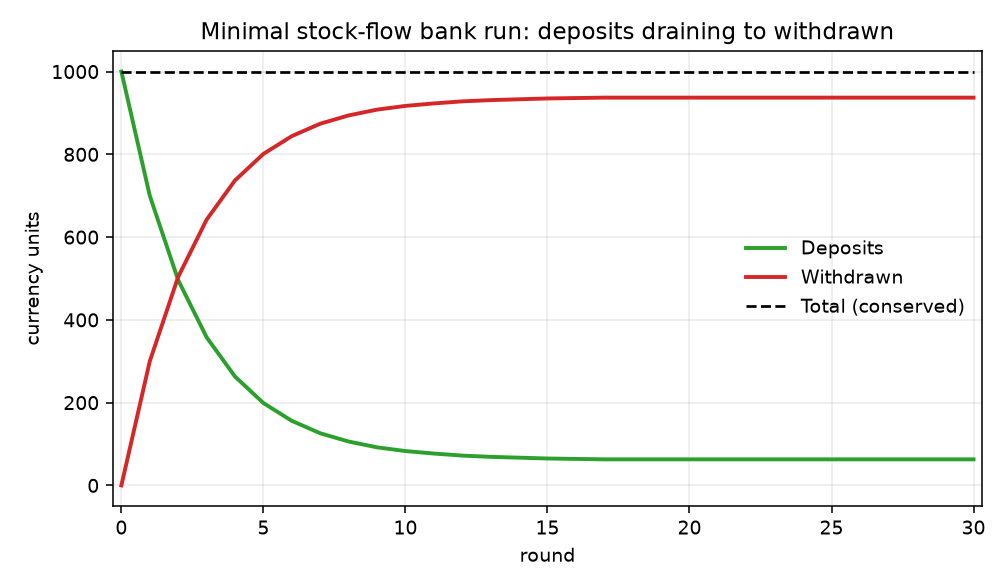
\includegraphics[width=0.72\textwidth]{figures/lethain_bankrun.png}
\caption{A minimal lethain stock-flow bank run: deposits drain into a withdrawn stock under a confidence-dependent leak, with a small return flow, and the total is conserved throughout. This is the bare ledger underneath the reflexive coupling of \S\ref{sec:reflexivity}; the basin-selection dynamics that decide \emph{whether} the run happens live in Fig.~\ref{fig:fixedpoints}, not here. An illustrative stock-flow schematic of the conserved-reallocation skeleton.}
\label{fig:lethain_bankrun}
\end{figure}

Two facts of the running example must be stated precisely, because they sharpen rather than undercut the thesis. First, \emph{standard} deposit insurance did not select the no-run equilibrium here: roughly ninety-four percent of SVB's \emph{domestic} deposits were uninsured at year-end 2022 (the relevant base, since foreign deposits were a small share), far above the standard 250{,}000-dollar cap, held by the same depositors whose roughly fifteen billion dollars in marked-down held-to-maturity assets (the \S\ref{sec:intro} fundamental) gave the run something real to run from, so the device that actually selected no-run was the discretionary systemic-risk exception of Sunday, March~12, 2023, an all-deposit backstop. That is not a standing rule but an exercise of discretion, the ex-post-optimal deviation whose anticipation is the classic time-inconsistency and moral-hazard problem \cite{kydlandprescott1977} (the live policy form being the lender of last resort's deliberate constructive ambiguity), issued at peak susceptibility, which is exactly the control-at-criticality story of \S\ref{sec:control} rather than a clean pre-committed fixed point. Second, Diamond--Dybvig is a pure-sunspot model, whereas SVB was a \emph{fundamentals-plus-panic} run, the interest-rate markdown of held-to-maturity assets being a real solvency shock that the panic then amplified. The modern refinement that captures this is the global-games selection of Goldstein and Pauzner \cite{goldsteinpauzner2005}, applying the global-games method of Carlsson and van Damme \cite{carlssonvandamme1993} (with Morris and Shin \cite{morrisshin1998} the currency-attack instance): a \emph{vanishing} amount of private-information noise, small relative to the dispersion of fundamentals, selects a unique equilibrium and a well-defined, fundamentals-increasing \emph{probability} of a run (the one-sided strategic-complementarity structure of demand deposits being what lets the global-games selection apply at all), which is the economist's version of our monotone-versus-imitative split and a sharper engineered-fixed-point story than 1983 sunspots. The art, then, is not predicting the future despite the audience. It is selecting, from among the futures consistent with the audience's reaction to hearing them, the one to announce. We name that selection plainly: when equilibria are multiple, choosing which self-fulfilling prophecy the population will live inside is an exercise of power, legitimate only under the conditions of \S\ref{sec:governance}, and not a neutral engineering act.

This inverts the secrecy requirement of the original specification. Seldon hid the \emph{contents} of the Plan while deliberately placing its \emph{existence} into the public record through the trial (the trial of \emph{Foundation}, 1951): the trial converted the Plan's existence into common knowledge precisely so that the Foundation's confidence in it became self-fulfilling, while the contents stayed sealed to prevent gaming. In our terms, the publishable set is the set of forecasts whose publication moves the population onto a stable equilibrium it is not yet on, whether by \emph{creating} the fixed point (a self-fulfilling forecast not yet a fixed point, consistent with the Diamond--Dybvig paragraph above, where ``no depositor will lose money'' is true only once announced) or by \emph{making an existing fixed point common knowledge} (true but not yet common knowledge, which is exactly what the trial published), while the withheld set is the multiple-equilibrium and self-defeating components. A forecast already a fixed point of common knowledge needs no publishing; it is inert. Information release is itself a control input; see \S\ref{sec:control}.

Two caveats bound the repair. First, MFG equilibria need not be unique. Multiple self-consistent prophecies can coexist, and the formalism selects among them no better than history does. We regard non-uniqueness as descriptive accuracy rather than failure, since coordination games genuinely have multiple equilibria, but it caps the resolution of equilibrium forecasting at the equilibrium \emph{set}. Second, the continuum hypothesis requires every agent to be of measure zero. Agents of non-negligible measure (platforms, states, central banks, and the out-of-distribution individual treated in \S\ref{sec:failure}) break the formalism and must be modeled as major players or as boundary conditions.

The condition that controls the first caveat is sharp. The Lasry--Lions \emph{monotonicity} condition on the coupling $F$ (here $\rho$ denotes the population density, written $m$ inside this integral to match the standard statement),
\begin{equation}
\int_X \big(F(x,\rho_1)-F(x,\rho_2)\big)\, d(\rho_1-\rho_2)(x) \;\geq\; 0
\qquad \text{for all } \rho_1,\rho_2\in\mathcal{P}(X)
\label{eq:monotone}
\end{equation}
with $\rho_1,\rho_2$ probability measures (so $\rho_1-\rho_2$ has zero total mass, which makes the pairing gauge-invariant) and $F(\cdot,\rho)$ bounded measurable, together with convexity of the Hamiltonian in the momentum variable, yields existence; \emph{strict} monotonicity (strict inequality whenever $\rho_1\neq\rho_2$) then yields a \emph{unique} MFG equilibrium, hence a unique publishable forecast \cite{lasrylions2007,carmonadelarue2018}. Interpreted, monotonicity is the congestion or strategic-substitutes regime: agents are repelled by the predicted crowd and avoid it, so the prediction is self-damping. When the coupling is instead \emph{imitative}, the strategic-complements regime in which agents pile into the prediction (bubbles, bank runs), Eq.~\eqref{eq:monotone} fails, and equilibria become multiple and bistable \cite{bardifischer2019}. Rule of thumb: when a crowd avoids what is predicted, prediction works; when a crowd chases it, only control works. The global-games program (Carlsson and van Damme \cite{carlssonvandamme1993}; \cite{morrisshin1998,goldsteinpauzner2005}) is the economist's route through the multiplicity, using a vanishing sliver of private-information noise, small relative to the dispersion of fundamentals, to pin a unique fundamentals-indexed threshold inside the otherwise imitative regime (uniqueness being a small-noise property, not a consequence of arbitrary noise). This yields the key synthesis of the section. The monotone (unique, predictable) versus imitative (multiple, unpredictable) split is the \emph{same boundary} as smooth versus critical: forecasting works in the monotone regime, and control takes over in the imitative one. Here we surface the genuine disagreement with strong reflexivity: Soros \cite{soros1987} holds the imitative, never-settling regime to be \emph{generic} in financial markets (boom and bust as the normal case), whereas our framework's empirical bet is that the imitative regime, while it accounts for a disproportionate share of realized variance and of the consequential moves (the fat tail), is the \emph{exception} rather than the generic state even in financial markets. That is a falsifiable difference, registered as the regime-occupancy test (the Soros bet) of \S\ref{sec:limits}, not a definitional evasion. The reflexivity repair therefore connects directly to the prediction--control duality of \S\ref{sec:control}, which is the imitative regime named in physical rather than game-theoretic language.

\paragraph{What the fixed-point repair does not fix.} The construction above answers the publication or observer effect, not the Lucas critique proper (\S\ref{sec:objections}, O2). The engine's calibrated coefficients ($\theta_S$, $v_k$, $D_k$, $W$, $\Phi$ of \S\ref{sec:engine}) are estimated against a historical record, and they are precisely the reduced-form, regime-dependent objects Lucas warns are non-invariant: a coefficient fit under one policy or platform regime carries no guarantee under another, and secrecy does not rescue it. The fixed-point machinery is silent on this. The only mitigation the engine offers is the online re-assimilation of \S\ref{sec:engine}, which continuously re-estimates only the identifiable subset $\{\theta_S, v_k, D_k, W\}$ as the regime drifts (the learning-toward-equilibrium posture of \cite{hansensargent2008}); the herding potential $\Phi$ is held to offline estimation as under-identified (\S\ref{sec:engine}), so its regime drift is precisely the residual the mitigation does not reach. This mitigates the exposure without eliminating it: assimilation lags regime change, and a sharp regime break leaves the engine briefly but genuinely miscalibrated. We register the structural non-invariance of these coefficients as a falsification condition in \S\ref{sec:limits}.

\section{Effective $N$ from near-decomposability}
\label{sec:blocks}

\subsection{Correlation is local}

The synchronization objection (O3) assumes mass media correlate \emph{everyone}. The empirical record of the platform era looks different. Global connectivity produced not one synchronized population but a proliferation of densely connected, mutually sparse communities. Tribes, in short. We argue this is a structural regularity rather than an accident of platform design. Simon's analysis of complex systems \cite{simon1962} holds that systems which persist under selection are \emph{nearly decomposable} hierarchies: interaction densities are high within subsystems and weak between them, because full global coupling is thermodynamically and organizationally unaffordable. Self-organizing systems autocorrelate \emph{locally}. Modularity is the equilibrium of that tendency. It is a pleasing regularity of the present program that both its conservation law and its independence structure originate with Simon, sixteen years apart.

\subsection{Near-decomposability as a conditional theorem}
\label{sec:nearcond}

The Simon appeal as just stated is an affordability hand-wave: full coupling is expensive, therefore systems are modular. That is suggestive, not a theorem, and near-decomposability is the load-bearing premise of the whole law-of-large-numbers repair (O3), so it deserves more than an assertion. We upgrade it to a \emph{conditional} statement: persistent modular (tribal) structure is a stable equilibrium provided three premises hold, each of which is independently defensible, and we are explicit that the conclusion is no stronger than the weakest of them. The point of stating it conditionally is that the third premise below is empirically at stake, and the theory predicts its own breakdown exactly when that premise fails.

\begin{enumerate}[label=(\alph*),itemsep=3pt]
\item \emph{Modularity from wiring cost.} Full pairwise coupling among $N$ units is $O(N^2)$ in connections and therefore unaffordable under any per-connection cost. Under selection with such a cost, the stable topology is modular, dense within blocks and sparse between them, rather than uniformly coupled: this is the evolutionary-origins-of-modularity result of Clune, Mouret, and Lipson \cite{clune2013}, in which adding a direct cost on connections is by itself sufficient to make modular networks the selected outcome. The Simon affordability intuition becomes a derived equilibrium of a cost-penalized selection process rather than a posited one.
\item \emph{Kuramoto sub-criticality.} Modularity in the wiring does not by itself keep blocks dynamically independent; weakly coupled oscillatory blocks can still lock. The mean-field Kuramoto result \cite{strogatz2000} is that full synchronization requires the coupling to exceed a critical value
\begin{equation}
K_c \;=\; \frac{2}{\pi\, g(0)},
\label{eq:kc}
\end{equation}
with $g$ the distribution of natural frequencies across blocks ($g(0)$ its density at the mean): for coupling $K<K_c$ the order parameter $r$ of \S\ref{sec:blocks} stays near zero and the blocks remain desynchronized, while for $K>K_c$ a macroscopic synchronized cluster forms and $r$ grows. Persistent decomposition is therefore precisely the \emph{sub-critical} phase $K<K_c$ of the same Kuramoto problem that supplies the synchrony observable $r$ feeding Eq.~\eqref{eq:kish}. Here $K_c$ and the $\lambda_c$ of \S\ref{sec:criticality} are the same boundary written in two notations.
\item \emph{Adversariality, not mere independence.} Independence between blocks would already suffice for the law of large numbers, but the platform record shows something stronger and more stable: blocks are not merely separate, they are \emph{adversarial}. This follows from conservation. Attention is the conserved, zero-sum resource of \S\ref{sec:attention}, so between blocks competing for a fixed total the competitive allocation is the Nash equilibrium, and an in-group/out-group disposition (cooperate within, contest without) is an evolutionarily stable strategy in the group-competition game in the sense of Maynard Smith and Price \cite{maynardsmith1973}. Adversarial tribalism is thus not an accident of polarization but a consequence of resource conservation plus group-competition game theory: conserved attention turns block independence into block rivalry.
\end{enumerate}

\paragraph{Synthesis: the World Cup and the hive.} Read together, the three premises place the population in a definite phase and name its boundary. The regime of many adversarial, sub-critically coupled blocks ($K<K_c$, premises (a)--(c) all holding) is a \emph{World Cup}: a fixed roster of rival tribes, each internally coherent, contesting a conserved pool of attention, none synchronized with the others. The opposite regime, in which the coupling has crossed $K_c$ and every block locks into one synchronized cluster, is the single-block hive we call \emph{Pluribus}: many bodies, one motion, $N_{\mathrm{eff}}\to 1$ by construction. This is exactly Asimov's Galaxia limit (\S\ref{sec:mule}). The two regimes are the two phases of Eq.~\eqref{eq:kc} separated by $K_c$, and that boundary is the \emph{same} boundary as the smooth-versus-critical transition of \S\ref{sec:criticality} and the monotone-versus-imitative split of \S\ref{sec:reflexivity}: one critical coupling, three names. Psychohistory is valid only in the World Cup phase, where blocks supply a real effective $N$, and it fails at Pluribus, where the effective $N$ collapses to one. Near-decomposability is therefore the precondition of the theory, and the theory predicts its own breakdown when the coupling crosses into the hive. We state the logical status plainly: this is a conditional theorem, not a free axiom and not an unconditional law. Premise (b), sub-criticality, is the condition genuinely at stake, since attention-routing technology can raise the effective coupling, and \S\ref{sec:instantiation} returns to the case in which it is pushed past $K_c$ deliberately.

\subsection{Renormalization to blocks}

The repair of O3 is a coarse-graining argument, the same move meteorology makes when it forecasts grid cells rather than molecules. This is also Seldon's own statement of the premise: psychohistory's foundational analogy, given in \emph{Foundation and Earth} (1986), is that one cannot predict the motion of a single gas molecule but, given enough of them, can predict the behavior of the gas, and our molecules-to-grid-cells move is that analogy made operational. No weather model tracks individual air molecules. It tracks the aggregate state of boxes of atmosphere, because within a box the molecules are strongly coupled and hopeless to track, while between distant boxes the coupling is weak and therefore statistical. The social analogue: do not model persons, model communities. Define blocks $B_1,\dots,B_K$ at the community scale (families, congregations, professional and ideological tribes, nations, at successive levels). Intra-block dynamics are fast and strongly coupled. Inter-block coupling is weak and matters only on long timescales. The statistical unit of the law of large numbers is the \emph{block}, not the individual. The effective number of independent units,
\begin{equation}
N_{\mathrm{eff}} \;\approx\; K \;\ll\; N_{\mathrm{pop}},
\end{equation}
is orders of magnitude smaller than $N_{\mathrm{pop}}$ and is estimable per corpus via community detection rather than assumed. The precise value of $K$ is a resolution-dependent output of the detection method, not a constant of nature; we decline to commit to ``thousands'' as a derived figure. That this is smaller than Seldon assumed is the point, and even a modest $K$ is ample for aggregate statistics in the weakly coupled regime. A simplification to flag: Eq.~\eqref{eq:kish} uses a single scalar $\varrho$ across all blocks, whereas the coupling matrix $W$ of \S\ref{sec:engine} is block-varying; a fully faithful treatment carries a block-varying $\varrho_k$, and the scalar form is a deliberate first approximation.

A methodological note on how $N_{\mathrm{eff}}$ is actually measured, since the naive choice is misleading. The point of the formula that follows is simple: if thousands of communities all start moving in lockstep, the effective number of independent units quietly collapses toward one, and aggregate statistics stop working; the formula just makes that precise, and a reader need not parse the $e^{\mathrm{i}\theta}$ to get the idea. For $K$ units sharing an intraclass correlation $\varrho$ (a variance-ratio statistic, distinct from the attention density $\rho$), the effective number of independent units is the Kish design-effect form
\begin{equation}
N_{\mathrm{eff}} \;=\; \frac{K}{1 + (K-1)\,\varrho},
\label{eq:kish}
\end{equation}
which recovers $N_{\mathrm{eff}}\approx K$ at $\varrho\to 0$ and collapses toward $1$ as $\varrho\to 1$ \cite{kish1965}. The right synchronization observable to drive $\varrho$ is the Kuramoto order parameter $r = \big|\,\frac{1}{K}\sum_k e^{\mathrm{i}\theta_k}\,\big|$ (lowercase $r$, the phase coherence, is unrelated to the uppercase observation-error covariance $R$ of \S\ref{sec:engine}), a first-moment phase-coherence statistic analogous to the mean-field magnetization of the block phases \cite{strogatz2000}. We must be careful here, because a garbled version of this point is easy to state. The Kish $\varrho$ is a second-moment intraclass correlation, whereas $r$ is a first-moment phase coherence; they are different objects, and $r$ cannot simply be substituted for $\varrho$ in Eq.~\eqref{eq:kish}. They are related by a model-dependent, nonlinear, monotone map $\varrho = g(r)$: under the mean-field factorization of phases conditional on the order parameter, the pairwise coherence of two distinct blocks equals $r^2$ \emph{exactly} (no Gaussian closure is needed, only the i.i.d.-given-$r$ factorization), and mapping that coherence onto the Kish intraclass $\varrho$ is the single model-dependent step, which is what feeds Eq.~\eqref{eq:kish} a genuine correlation. The reason to track $r$ (and the macroscopic variance-ratio that also responds) rather than the raw Pearson correlation of fluctuations is that $r$ is bounded, mean-field, and saturates cleanly at synchrony, moving from near $0$ in the decoupled regime to near $1$ at full synchronization. By contrast, under \emph{well}-synchronization the Pearson correlation of fluctuations \emph{around} the common trajectory stays near \emph{zero} (the residual jitter is what is left after the shared motion is removed), so a naive $N_{\mathrm{eff}}$ built from that correlation fails to fall even as independence collapses. The order parameter $r$ and the macro variance-ratio detect the collapse that the fluctuation correlation misses.

Individuals re-enter as superpositions. Each person $i$ carries a membership vector $\pi_i \in \Delta^{K-1}$ over blocks (family $\oplus$ religion $\oplus$ nation $\oplus$ profession $\oplus$ \dots), which is the mixed-membership stochastic blockmodel \cite{airoldi2008}: identity as a convex combination of tribal belief vectors. A person is, for predictive purposes, a weighted mixture of the communities that raised, employ, and surround them. Practically dependent on each; formally captured by none alone. Both the blocks and the memberships are estimable from interaction graphs by community detection, so the decomposition is an empirical object, not a modeling convenience. The running example illustrates block structure cleanly in its opening phase. The run propagated in hours \emph{within} one professional community and its shared platform, while depositor communities outside that block initially did not move at all. The inter-block coupling appears, at first, to have been perturbatively weak, which is the regime in which block statistics are valid; we note this is a narrative reading of one episode, not a measured cross-block correlation. What happened next is \S\ref{sec:criticality}. The game-theoretic layer generalizes accordingly to multi-population mean-field games, one density $\rho_k$ per block coupled by weak interaction terms, an established extension of the formalism.

\paragraph{Relation to cliodynamics.} It is worth positioning this program honestly against the closest existing real attempt at a predictive social science, Peter Turchin's cliodynamics and its structural-demographic theory \cite{turchin2003,turchin2016}. That program models slow structural aggregates (popular immiseration, elite overproduction, state fiscal stress) with decadal lags, and it issued at least one published forward statement \cite{turchin2010}, a structural forecast of elevated instability in the 2020s. We are careful not to oversell it: that is a single, not-yet-validated out-of-sample forecast, and structural-demographic theory carries well-known overfitting and degrees-of-freedom objections (the elite-overproduction index is in part constructed with hindsight). The same prosecutor's-fallacy standard we apply to early-warning signals in \S\ref{sec:criticality} applies symmetrically to cliodynamics' in-sample historical calibration, so we treat its data advantage as real but not unalloyed. Cliodynamics \emph{explicitly disclaims} predicting individuals or triggers, conceding that at the level of who lights the match and when, prediction fails. We adopt, in the paper's own voice, the formulation that at the trigger scale \emph{we are all Mules}: the slow aggregates are the smooth, monotone regime, and the trigger is the critical, imitative one, and this structure-versus-trigger split is what the present paper formalizes as the prediction--control duality. What we add over cliodynamics is the ensemble and assimilation machinery of \S\ref{sec:engine}, the reflexivity treatment via mean-field games (\S\ref{sec:reflexivity}), and the explicit criticality apparatus (\S\ref{sec:criticality}). What it has and we do not is the decisive asset: state variables calibrated on real historical data.

\section{The predictive engine}
\label{sec:engine}

Sections~\ref{sec:attention}--\ref{sec:blocks} repaired objections; they did not state the machine. We now define the engine as a state-space system in the standard filtering form (forward model, observation operator, assimilation update, ensemble forecast) so that every repair above appears as a component with a defined interface. For readers who want the shape before the symbols: the engine runs like a weather bureau. It maintains a best estimate of the current social weather, meaning where each community's attention sits and which way belief is pulling it. Several times a day it corrects that estimate against fresh observations. It then runs many slightly perturbed copies of the model forward and reports the \emph{spread} of those copies as the forecast, together with an honest statement of how far ahead the forecast beats historical base rates. Nothing in the loop is exotic. What is new is only the model being looped.

\subsection{State}

The state bundles the slow macro stocks with one attention density and belief field per block, the inter-block coupling, the memberships, and the explicit major players. The full state at time $t$ is
\begin{equation}
\Xi_t \;=\; \big(\, S_t,\; \{\rho_k\}_{k=1}^K,\; \{b_k\}_{k=1}^K,\; W,\; \Pi,\; \{q_\ell\}_{\ell} \,\big),
\end{equation}
where $S_t \in \mathbb{R}^m$ are slow macro stocks (demographics, debt, energy, aggregate attention supply $A$); $\rho_k$ is block $k$'s attention density over the topic space $X$; $b_k$ its belief field; $W \in \mathbb{R}^{K\times K}_{\geq 0}$ the slowly varying inter-block coupling matrix; $\Pi = (\pi_i)$ the mixed-membership matrix of \S\ref{sec:blocks}; and $\{q_\ell\}$ the explicit \emph{major-player} states. This last component is not a cosmetic addition. \S\ref{sec:reflexivity} conceded that agents of non-negligible measure (platforms, states, central banks) break the continuum hypothesis, and every actor that \emph{acted} in the running example (the regulator who issued the guarantee, the platform over which the run propagated) is exactly such a player. They are therefore carried as first-class finite-measure states coupled to the mean-field, not relegated to a caveat; the engine has a slot for the one who pulls the lever.

In practice $X$ is not a continuum. Topics are embedded, for instance by a text encoder, then clustered into a graph $G=(V,E)$ of $|V|=n$ topic nodes, and each density becomes a probability vector $p_k \in \Delta^{n-1}$. The differential operators of \S\ref{sec:attention} become graph operators, and the transport PDE becomes a master equation. Several quantities here are open specification points rather than settled choices, and we label them as such: the topic graph $G$ (node count $n$, and whether the node set is static or churns as topics are born and die, which requires an explicit mass-reassignment rule on node deletion so the conservation bookkeeping of Eq.~\eqref{eq:continuity} is not violated, plus an edge definition, semantic-similarity kNN being one reference choice, that silently fixes the diffusion operator), the total state dimension (which scales as $O(Kn + K^2 + N_{\mathrm{pop}}K)$: roughly $K\,n$ for the densities, $W\sim K^2$, and the membership matrix $\Pi$ at $N_{\mathrm{pop}}\times K$, which for $N_{\mathrm{pop}}\sim10^8$ is the dominant term by orders of magnitude; $\Pi$ is therefore not carried in the assimilated state but factored out into the observation operator $\mathcal{H}$, which aggregates block densities through it, leaving the assimilated state at $O(Kn+K^2)$, so localization and inflation of the ensemble covariance are mandatory, not optional, and the per-cycle cost must be budgeted against this), and the non-unique MFG-closure selection rule discussed below. We do not resolve these here; we pin them as the named gaps an implementation must close.

\subsection{Forward model}

The model $\mathcal{M}$ advances $\Xi_t \mapsto \Xi_{t+\delta}$ through three coupled layers, ordered by timescale.

\paragraph{Slow layer (stocks).} Macro stock-and-flow dynamics,
\begin{equation}
\dot S = F_S(S; \theta_S),
\end{equation}
with $F_S$ the standard system-dynamics form \cite{forrester1961,sterman2000} (the management-practice exposition of \cite{larson} is a motivating reference, not the formal authority). This layer is reliable and low-dimensional, and it supplies the source terms $s_k$ and the total supply $A(t)$ to the layer below.

\paragraph{Fast layer (transport).} Per-block attention transport on the topic graph, the discretization of Eqs.~\eqref{eq:continuity}--\eqref{eq:flux}:
\begin{equation}
\frac{d p_k}{dt} \;=\; L(b_k)^{\!\top} p_k \;+\; \sum_{j \neq k} W_{kj}\,(p_j - p_k) \;+\; s_k,
\label{eq:master}
\end{equation}
where $L(b_k)$ is a rate matrix (the graph generator, with $\nabla_G$ the graph gradient and the diffusion term supplied by $-\mathcal{L}_{\mathrm{graph}}$, the \emph{negative} of the positive-semidefinite graph Laplacian $\mathcal{L}_{\mathrm{graph}}=D-A$, so the off-diagonal rates are non-negative and the diffusion relaxes $p_k$ toward uniform rather than amplifying it) whose edge rates combine baseline drift $v_k$, diffusion $D_k$, and the belief bias $b_k$ along edges of $G$. Each row of $L$ sums to zero, so $L\mathbf{1}=0$ and $\mathbf{1}^\top \dot p_k = \mathbf{1}^\top L^\top p_k = (L\mathbf{1})^\top p_k = 0$: Eq.~\eqref{eq:master} conserves $\mathbf{1}^\top p_k$ up to the explicit source and exchange terms, and the transpose convention is what makes this hold. The conservation law of \S\ref{sec:attention} is enforced \emph{structurally} rather than as a soft constraint. One condition must be stated, because row-sum-zero is necessary but not sufficient for $p_k$ to remain a probability vector: $L(b_k)$ must have non-negative off-diagonal entries and zero row sums (a constraint on how strongly $b_k$ may bias an edge rate), so that its transpose $L^\top$, the operator that actually drives $p_k$, is a continuous-time Markov generator (Metzler, zero column sums) under which $p_k$ stays in the simplex $\Delta^{n-1}$ and does not merely remain on the affine hyperplane $\mathbf{1}^\top p_k = 1$ while a component goes negative. The exchange term $\sum_j W_{kj}(p_j-p_k)$ is the weak coupling of \S\ref{sec:blocks}, and the regime monitor of \S\ref{sec:control} watches whether this term remains perturbative.

\paragraph{Belief layer (closure).} The constitutive decomposition of \S\ref{sec:attention} closes the system:
\begin{equation}
b_k \;=\; b_k^{\mathrm{ext}}(t) \;+\; \beta_k \,\nabla_G \phi_k \;+\; b_k^{\mathrm{strat}},
\qquad \phi_k \;=\; -\,\frac{\partial \Phi}{\partial p_k} \;=\; M p_k,
\label{eq:closure}
\end{equation}
with $\nabla_G$ the graph gradient and $\phi_k$ a node-indexed potential field over the topic graph (so the gradient operator and its argument live on the same node space). The exogenous term is an input stream, an events feed. The endogenous term is herding on the current attention configuration; a concrete reference choice for the underlying scalar is $\Phi(p_1,\dots,p_K) = -\tfrac{1}{2}\sum_k p_k^\top M p_k$ with $M$ a positive affinity matrix on topic nodes, whose per-block variation $\partial\Phi/\partial p_k = -M p_k$ gives the node field $\phi_k = M p_k$, so that $\nabla_G\phi_k$ pulls attention toward already-popular and semantically adjacent nodes (preferential attachment), and the sign and curvature of $M$ are what place the system in the monotone or imitative regime of \S\ref{sec:reflexivity}.

The strategic term comes from solving the multi-population MFG of \S\ref{sec:reflexivity} to an equilibrium given the current state, and this is the most expensive and least innocent step in the loop. Two honest statements are required. First, the cost: solving a coupled HJB/Fokker--Planck system for $K$ populations is itself a fixed-point PDE solve, and doing it once per ensemble member per assimilation cycle is a triple-nested loop whose budget an implementation must check; in the smooth monotone regime the solve is a contraction and converges, which is the regime where the engine is meant to run open-loop. Second, the selection: in the imitative regime, which by the synthesis of \S\ref{sec:reflexivity} is the \emph{same} boundary as criticality, the equilibrium is not unique, so the forward model must \emph{select} one branch to integrate. That selection is a control choice, not a dynamical step, and the engine must declare it (a stated refinement or history-dependence rule, with the branch selection reported as an input to the forecast, not hidden inside the parenthetical ``an''). When the closure fails to converge, which is the diagnostic of the imitative regime, the engine does not paper over it; it triggers the mode switch of \S\ref{sec:control}. The HJB layer is thus evaluated \emph{inside} the forward model, so published forecasts are fixed points by construction rather than by audit, conditional on the declared branch.

\subsection{Observation operator and assimilation}

Observations $y_t$ (platform engagement metrics, surveys, prediction-market prices, mobility and sales data) relate to the state by $y_t = \mathcal{H}(\Xi_t) + \varepsilon_t$, $\varepsilon_t \sim \mathcal{P}_R$ (an observation-error law to be specified), where $\mathcal{H}$ (written with a script symbol to distinguish it from the Hamiltonian $H$) aggregates block densities through the membership matrix $\Pi$. An individual-level signal is a $\pi_i$-weighted mixture of block states. We flag at once that the observation model is where a v0 actually breaks, and that the single line above hides the hardest engineering. The Gaussian-additive choice $\varepsilon_t\sim\mathcal{N}(0,R)$ is the placeholder we adopt for the consistency checks of \S\ref{sec:figures} only, and it is almost certainly wrong for engagement data, which are heavy-tailed, bot-contaminated, and reflexively gamed. The strategic layer of \S\ref{sec:reflexivity} means the observations are themselves adversarial, a problem ordinary filtering does not handle and which we name as a first-class open problem rather than absorb into $R$. Mapping even one concrete source (say platform engagement to block attention mass) to a $\pi_i$-weighted mixture is a research project per data source, and $R$ must be estimated, not posited; in NWP a mis-specified $R$ is the classic route to filter divergence.

The engine is never free-run. On each cycle, an ensemble $\{\Xi^{(e)}\}_{e=1}^{E}$ is propagated through $\mathcal{M}$, the predicted-observation ensemble $Y_f^{(e)} := \mathcal{H}(\Xi_f^{(e)})$ is formed, and the state is corrected by the ensemble Kalman filter (EnKF) analysis
\begin{equation}
\Xi^{(e)}_a \;=\; \Xi^{(e)}_f \;+\; \widehat{\mathrm{cov}}(\Xi_f,Y_f)\,\big(\widehat{\mathrm{cov}}(Y_f,Y_f) + R\big)^{-1}\big(y_t + \eta^{(e)} - Y_f^{(e)}\big),
\label{eq:enkf}
\end{equation}
with the ensemble cross- and auto-covariances $\widehat{\mathrm{cov}}(\Xi_f,Y_f)$ and $\widehat{\mathrm{cov}}(Y_f,Y_f)$ of the state and the predicted-observation ensembles replacing the explicit gain $\hat P_f \mathcal{H}^\top(\mathcal{H}\hat P_f \mathcal{H}^\top + R)^{-1}$ of the linear case (to which they reduce when $Y_f=\mathcal{H}\Xi_f$ is linear), since $\mathcal{H}$ is nonlinear, and $\eta^{(e)} \sim \mathcal{N}(0,R)$ perturbed observations. With a small ensemble $E$ the sample covariance is rank-$E$ and demands localization and inflation, which are mandatory here, not optional. Equation~\eqref{eq:enkf} is, in words, a disciplined compromise. Each ensemble member is nudged toward what was actually observed, by an amount that weighs how uncertain the model is against how noisy the data are. Parameters are estimated offline against a historical \emph{social reanalysis} corpus (described next) and refined online by augmented-state assimilation; we restrict the online-estimated set to the low-dimensional, identifiable parameters ($\theta_S$, the scalar diffusion and drift magnitudes, $W$) and hold the high-dimensional or weakly identified objects (the herding potential $\Phi$ and the error covariance $R$) to offline estimation, because appending a whole potential and a covariance to the EnKF state is under-identified. These calibrated coefficients are exactly the reduced-form, regime-dependent objects the Lucas critique (\S\ref{sec:objections}, O2) targets; online re-assimilation tracks their drift but does not make them structurally invariant, so the engine is exposed to Lucas non-invariance and only partially mitigates it \cite{hansensargent2008}.

\paragraph{Misspecification monitor.} The skill horizon below is an in-model object and is therefore silent about the out-of-model (Mule) failure of \S\ref{sec:mule}. The engine must carry a separate diagnostic for it: an observation-innovation / ensemble-rank monitor that watches for assimilation innovations $y_t - \mathcal{H}(\Xi_f)$ that the filter cannot reduce, persistently, across cycles (equivalently, a degenerate rank histogram). Persistent irreducible innovation is the only in-loop signature of an agent the model class does not contain. This makes out-of-distribution failure at least \emph{detectable} after the fact, though never anticipable, and it is why the horizon $\tau^\ast$ below must be reported as conditional on no out-of-model agent.

\paragraph{The social reanalysis corpus.} The corpus is the single largest missing piece of infrastructure for this program, and we specify it as an artifact rather than confess it as a gap. A single record is a tuple $(\text{timestamp},\ \text{block id},\ \text{topic-graph node},\ \text{attention-mass estimate},\ \text{belief/valence estimate},\ \text{inter-block coupling estimate},\ \text{observation-stream provenance},\ \text{observation-error estimate})$. The corpus must span enough regimes and resolve a fine enough cadence to identify a Lyapunov rate and a $K\times K$ coupling matrix $W$, which a single year of data cannot do; the order of magnitude is many years of daily-or-faster block-level records with stable block identity across the span (and block identity is itself non-stationary, since communities merge, split, and rename, so a block-tracking and identity-stitching rule is a named prerequisite). The fatal and usually hidden difficulty is a co-bootstrap: ERA5 was built by assimilating instrument-grade observations into a \emph{trusted} physical model, whereas here there is neither a trusted forward model nor instrument-grade observations, so the corpus and the model must be built from each other, a chicken-and-egg the program cannot wish away. We therefore state plainly that the program is, until this corpus exists, design ahead of data: the engine is a specification, and \S\ref{sec:implementation} is a build plan, not a report. NWP skill followed the reanalysis datasets, not the other way around.

\subsection{Forecast operator and skill horizon}

A forecast at lead time $\tau$ is the pushforward of the analysis ensemble, reported as a distribution and scored by the continuous ranked probability score (CRPS) and Brier score at resolution \cite{tetlock2015}. The ensemble doubles as the engine's own error model. The \emph{skill horizon} $\tau^\ast$ is defined operationally as the \emph{least} lead time $\tau$ at which forecast spread first equals or exceeds climatological (base-rate) spread (spread growth near criticality need not be monotone, so the least crossing time is the operative one). We are deliberate about what $\tau^\ast$ is and is not. It is an empirical spread-crossing (degradation) time; it is \emph{not} reliably a Lyapunov horizon, because ensemble spread growth has two distinct generators the ensemble cannot tell apart: genuine chaotic divergence of a \emph{correct} model, and the coefficient breakdown of \S\ref{sec:criticality}(c), where coefficients calibrated in the smooth regime are simply \emph{wrong} in the critical one (the model becoming false, not merely chaotic). We therefore report $\tau^\ast$ as a degradation time whose cause the engine cannot self-diagnose, and we stop attributing it to a leading Lyapunov exponent. Beyond $\tau^\ast$ the engine reports base rates, by construction. $\tau^\ast$ is state-dependent: as the system approaches criticality (\S\ref{sec:criticality}), spread growth accelerates and $\tau^\ast \to 0$, which is the signal that triggers the mode switch of \S\ref{sec:control}.

Crucially, $\tau^\ast$ covers only the aleatoric (pure chance, the luck of the draw), in-model half of unpredictability. It is conditional on there being no out-of-model (Mule) agent, and that condition is unanticipable from inside the loop, detectable only in arrears by the misspecification monitor, and never falsifiable before the agent has already acted. An operator reading a single $\tau^\ast$ would believe he holds a calibrated horizon when he holds only half of one; the engine must therefore emit $\tau^\ast$ \emph{together with} the misspecification-monitor flag above, so the two failure modes are reported separately. The engine does not merely degrade at criticality; it announces both its in-model degradation and, when detectable, its out-of-model misspecification as first-class outputs.

In summary, one cycle of the engine is: assimilate (Eq.~\ref{eq:enkf}), solve the MFG closure (Eq.~\ref{eq:closure}), integrate the ensemble forward (Eq.~\ref{eq:master}), emit predictive distributions together with the skill horizon and regime diagnostics, repeat. The remainder of the paper characterizes when this loop fails.

\section{Two failure modes, sharply distinguished}
\label{sec:failure}

The repairs of \S\S\ref{sec:attention}--\ref{sec:blocks} each carry a validity condition. We now characterize the regimes in which the conditions fail. There are two such regimes, and they are not the same phenomenon.

\subsection{Criticality: in-model unpredictability}
\label{sec:criticality}

Weak inter-block coupling is weak, not zero, and the coupled system has a correlation length $\xi$. Near a critical transition, $\xi$ diverges,
\begin{equation}
\xi \;\sim\; |\lambda - \lambda_c|^{-\nu},
\end{equation}
where $\lambda$ is the scalar coupling tuned across the transition (the inter-block coupling strength of $W$) and $\lambda_c$ its critical value, kept distinct from the calibrated-coefficient vector $\theta_S$ and the block phase $\theta_k$. As $\xi$ diverges, previously decoupled blocks synchronize, and the consequences arrive together:
\begin{enumerate}[label=(\alph*),itemsep=2pt]
\item $N_{\mathrm{eff}}$ collapses from roughly $K$ toward $1$ as the Kuramoto order parameter $r$ rises toward $1$ in Eq.~\eqref{eq:kish}. The recovered law of large numbers evaporates at the moment the stakes are highest: panics, mobilizations, cascades.
\item The MFG fixed-point repair fails. Critical transitions are non-equilibrium dynamics, cascades rather than fixed points, and they are frequently triggered or amplified by agents of non-negligible measure.
\item Conservation survives as bookkeeping but stops constraining. Attention is still conserved, indeed concentrated, during a panic, yet the drift term $\rho b$ becomes dominated by a single global gradient that swamps every coefficient calibrated in the smooth regime. We state the consequence without softening it: the low-effective-dimension benefit that conservation buys (\S\ref{sec:attention}) is a \emph{smooth-regime} benefit only. Conservation constrains the dynamics where they are already easy and stops constraining them exactly where forecasting is hard. It is not a repair that extends into the critical regime, and \S\ref{sec:attention} should not be read as implying otherwise; the continuity equation is bookkeeping, and bookkeeping never stopped a panic. The one consequence of conservation that must still hold at criticality, and is therefore a genuine falsifier (\S\ref{sec:limits}), is that total attention-minutes do not balloon on the sub-generational timescale of the panic, beyond the slow endogenous source term $s$ of Eq.~\eqref{eq:continuity}; they are reallocated, not created. The discriminating form is a closed within-window ledger: the rise in attention-minutes on the panic topic should equal, net of that slow source, the simultaneous fall on the displaced topics, so that a panic topic whose gain exceeds the measured losses elsewhere is net attention creation and refutes the law even with a stable grand total.
\end{enumerate}
Criticality is unpredictability \emph{within} a correct model. The dynamics are known; the sensitivity diverges. The physical metaphor is a magnet near its Curie temperature, or a stadium a moment before the wave; the gas of \S\ref{sec:blocks} was the smooth regime, where individuals are unpredictable but aggregable, and the stadium wave is what that same gas does at its Curie point, where they are coupled into one motion. Far from the transition, each region of the crowd does its own thing and a shove affects only the neighbors. At the transition, regions that never coordinated suddenly move as one, and the lone fan who stands up takes the whole stadium with him. The running example illustrates this boundary in its second phase. A run that had been confined to one professional block began, within a weekend, to synchronize depositor behavior at \emph{unrelated} regional banks. The framework's hypothesis is that blocks with no direct exposure moved together because the correlation length had changed rather than the fundamentals; we flag this as a hypothesis, not an established fact, because confirming it requires measuring a rising cross-block order parameter $r$, which we have not done for this episode. The fat tails of social history are not noise around the model. They are the regime in which the model's assumptions are the casualties.

One partial recovery is available. Critical transitions in driven systems are preceded by measurable precursors: critical slowing-down, rising variance, rising lag-1 autocorrelation, rising cross-unit correlation \cite{scheffer2009}. Rising synchrony between previously independent blocks is itself the alarm. The system's predictability is therefore a \emph{state variable}, and the model should report it as such. One can often predict \emph{that} a transition is imminent without predicting \emph{which branch} it takes. Early warning without trajectory.

These signals must be qualified honestly, because they are narrower than they are often taken to be. They are valid \emph{only} for slow bifurcation-induced (B-)tipping at fold-type transitions, and three failure modes defeat them. First, the prosecutor's fallacy: selecting series already known to have tipped and then ``finding'' the precursor conditions on the outcome, so that $P(\text{signal}\mid\text{transition}) \neq P(\text{transition}\mid\text{signal})$, and a null model together with the base rate is required before any signal can be scored \cite{boettiger2012}. Second, noise-induced (N-)tipping, in which a fluctuation carries the state across a basin boundary with no preceding loss of stability, hence no slowing-down to detect \cite{boettiger2013}. Third, rate-induced (R-)tipping, which involves no bifurcation at all (the system fails to track a moving stable state that is driven past too quickly) and therefore exhibits no precursor \cite{ashwin2012}. N- and R-tipping are explicit blind spots of the early-warning layer: the regime monitor of \S\ref{sec:control} can be silent right up to a transition of either type, and the architecture must not treat the absence of an early-warning signal as evidence of safety. This quietly bounds the whole program. The early-warning layer (and the entire pre-critical column of the \S\ref{sec:control} architecture) has predictive value only insofar as decision-relevant social crises are \emph{predominantly} fold-type B-tipping rather than N- or R-tipping, and that conjecture is currently unsupported. We promote it to the sharpest falsification test in \S\ref{sec:limits}, because it is the one most likely to fail: engineered crises (the kind a Plan designs for) are folds, but history's crises are not obliged to be courteous.

\subsection{Misspecification: out-of-model failure}
\label{sec:mule}

The second failure mode is categorically different. Asimov's Mule (in \emph{Foundation and Empire}, 1952), a mutant whose psychology lay outside the model class of the Seldon Plan, is not a chaotic excursion of known dynamics but a hypothesis-space error. The Mule's power is endogenous to himself, an emotional control no model anticipated, and he is the clean exemplar of an out-of-distribution agent: the generative process contained an agent type assigned zero prior mass. In contemporary terms, an out-of-distribution sample; in classical terms, epistemic rather than aleatoric uncertainty. The everyday version of the distinction: aleatoric uncertainty is not knowing which face a fair die will show, while epistemic uncertainty is not knowing that the object being thrown is not a die at all. More throws help with the first and are useless against the second. The distinction is operationally decisive, because the standard remedy for aleatoric error (more data, tighter assimilation) does nothing here. Additional observations of in-distribution agents carry no information about the existence of out-of-distribution ones. (We are careful with the canon here: the Mule, not Gaia, is the misspecification exemplar. Gaia is a separate and later device, treated under the patch sequence below; the Mule's existence could not have been inferred from the Plan's training distribution, and that is the whole point.)

A contrast with the running example sharpens the distinction, and closes the one place the SVB thread otherwise goes silent. SVB was \emph{not} a Mule. It was criticality, an in-model chaotic excursion (a run) of dynamics the framework contains, which is precisely why a single deposit-guarantee announcement could switch it off. A true Mule event, an agent outside the model class, would not yield to a fixed-point announcement at all, because the announcement is computed inside a model that does not contain the agent. The Mule is the disease; the patches below are proposed cures, and one must not let the cure contaminate the statement of the disease.

Asimov's own patch sequence is an argument worth reconstructing, with the firewall that his resolutions are narrative, not evidence: we use them only to \emph{name} failure modes, never as support that the modes are surmountable. The first patch is the Second Foundation (\emph{Second Foundation}, 1953). Abandon prediction of out-of-model events and maintain a standing \emph{corrective controller}, fast enough to re-converge the trajectory after detection. Online correction of the Plan, with the attendant problem that the controllers themselves become an unaccountable power; the later novels are explicitly about this, and from the controlled population's frame the corrective controller, operating at criticality with private information and a self-authored objective, is \emph{itself} the agent of non-negligible measure that breaks everyone else's model of their world. The corrective controller does not escape the out-of-distribution problem; it relocates the out-of-distribution agent into the control room. The terminal patch is Galaxia (chosen at the close of \emph{Foundation's Edge}, 1982, and interrogated throughout \emph{Foundation and Earth}, 1986: extending the planet-wide shared mind Gaia to the entire galaxy): collapse the distinction between model and world entirely. A system whose every component shares state admits no out-of-distribution agents by construction. Zero sim-to-real gap, purchased by abolishing independent agents altogether. $N_{\mathrm{eff}} \to 1$ by design, the pathology of \S\ref{sec:criticality} converted into the cure. And then Asimov makes the activation of Galaxia hinge on an external human chooser (Trevize, in the closing decision of \emph{Foundation's Edge}), because the controller cannot validate its own objective function at the decisive branch. The reason the final choice is given to a person and not to the Plan is that no system can certify the rightness of the world it is about to impose; that is the same wall the trilemma of \S\ref{sec:limits} hits. In retrospect this is a very early statement of the value-alignment problem, and we develop it as a structural requirement in \S\ref{sec:governance} and \S\ref{sec:limits}.

\subsection{The Second Foundation, derived}
\label{sec:secondfoundation}

The first of Asimov's patches, the Second Foundation, is usually read as a plot device. It is in fact forced by the misspecification structure above, and the derivation is short. We give it because it tells us exactly what kind of object the standing corrective controller must be, and why a smarter fixed model cannot replace it. The argument is control-theoretic and self-contained; we then exhibit the chain twice empirically, first as a \emph{real-data instance} on the live r/AskEconomics activity series and then as a clean \emph{synthetic schematic} of the same mechanism.

\begin{enumerate}[label=\arabic*.,itemsep=3pt]
\item \emph{Forecast error decomposes.} The one-step forecast error splits into an \emph{aleatoric} part (irreducible process and observation noise, variance set by the noise floor, which no controller can beat) and an \emph{epistemic} part (model-class error, the bias of the best in-class approximation over the operating regime). In-distribution the epistemic part is small, because that is the regime the model was fit on.
\item \emph{An out-of-distribution event makes the epistemic term $O(1)$.} After an out-of-distribution regime change, the truth contains a term lying outside the model's hypothesis class $\mathcal{H}$ (in the worked case a unit root plus a persistent drift, neither in the pre-shock class). The best in-class approximation then has a bias floor $\inf_{\hat f\in\mathcal{H}}\|\hat f - f'\| = O(1) > 0$, and \emph{no amount of additional in-distribution data shrinks it}: in-distribution data is by definition drawn from the pre-shock regime and is silent about the new term. The epistemic error is now $O(1)$ and irreducible by in-distribution data. This is the formal content of ``the model has a blind spot,'' and it is the Mule restated in estimation language.
\item \emph{Open-loop error then diverges.} Free-run the pre-shock model from the change-point $\tau$. With true post-shock growth rate $\lambda$, the forecast error grows as
\begin{equation}
e_t \;\sim\; |f' - \hat f|\,(t-\tau)\quad(\text{linear, unit-root drift}),
\qquad
e_t \;\sim\; e_0\,e^{\lambda(t-\tau)}\quad(\lambda>0,\ \text{Lyapunov form}),
\label{eq:openloop}
\end{equation}
linearly under a unit root and exponentially under a positive Lyapunov exponent. Either way the integrated error grows without bound.
\item \emph{No fixed controller suffices (Internal Model Principle).} Francis and Wonham \cite{franciswonham1976} established that a controller achieves asymptotic disturbance rejection only if it embeds a model of the disturbance's dynamics: the regulator must contain a copy of the exosystem generating the disturbance. But an out-of-distribution event is unmodeled by construction, its generator absent from the controller's internal model, so \emph{no fixed controller can asymptotically reject it}. Any controller with a frozen internal model has some out-of-distribution disturbance it fails to reject. The open-loop case (3) is the limiting instance: its internal model lacks the new term entirely, so its error diverges.
\item \emph{Therefore bounded long-run error requires an adaptive detect-and-correct loop.} If no fixed controller suffices (4) and open-loop diverges (3), then bounded error under arbitrary out-of-distribution shocks requires a standing loop that (i) \emph{detects} the change-point and (ii) \emph{re-identifies} the model online, expanding its internal model to embed the now-observed disturbance and so restoring the Internal Model Principle after the fact. Detection is change-point detection on the normalized innovation: a one-sided CUSUM \cite{page1954} on the normalized innovation squared, $g_t = \max(0,\,g_{t-1}+\mathrm{NIS}_t - k)$ flagged when $g_t>h$, which has negative drift while the model is correct (no false alarm) and positive drift only once the shock inflates the innovations. This is exactly the misspecification monitor of \S\ref{sec:engine} (the innovation-whiteness consistency test) promoted to a standing change-point-plus-re-identification loop. That standing adaptive controller \emph{is} the Second Foundation, and it cannot be replaced by a smarter fixed model, because the next out-of-distribution event is outside \emph{that} model too; the requirement is structural, not a matter of model quality.
\item \emph{Two properties follow for free.} First, the detection lag is positive: the monitor breaches threshold \emph{after} onset, so the loop repairs after the fact and cannot foresee the shock. The Mule wins the first move, matching Asimov exactly. Second, in a model \emph{monoculture}, models distilled from one base share the blind spot and so fail together, which makes a single centralized corrector both necessary (no lineage self-corrects) and most dangerous (it holds maximal control with minimal accountability), whereas \emph{model diversity} is partially self-correcting (if any independent lineage's class covers the novel term, the ensemble repairs at the closed-loop floor) and therefore substitutes for the central controller. The corrector is least dangerous precisely when it is least necessary.
\end{enumerate}

\paragraph{Real-data demonstration (primary evidence).} The chain is not only a synthetic construction; it runs on real data. The engine slice of \S\ref{sec:engine} executes the strictly causal walk-forward EnKF on the live r/AskEconomics monthly activity series, and its misspecification monitor flagged a genuine out-of-distribution break at 2025-04-30 with normalized innovation $z=-3.33$, the collapse to $946$ submissions after the sharp Jan--Mar 2025 ramp ($1238\to1332\to1872$), \emph{with no future information}. We take that real break and run the two arms of the argument directly on the real series. The open-loop arm fits the local-linear-trend model strictly before the ramp onset and free-runs it forward without assimilating; frozen at its pre-ramp trend it cannot follow the ramp, so across the divergence window (onset to the monitor flag) its integrated forecast error grows. The closed-loop arm is the EnKF assimilating each new observation through the break; it tracks the ramp and the monitor detects the break a few steps after onset. On the real series the open-loop integrated error over the divergence window is about $0.81$ (log units) against the closed loop's about $0.46$, a ratio of about $1.8$, and the detection lag is $3$ steps: the monitor breaches threshold at the April collapse and never before. We report one honest property of this particular series alongside the result: at the collapse step itself the frozen-flat open-loop happens to land near the post-collapse level while the ramp-tracking closed loop absorbs the full collapse surprise (the $z=-4.71$ innovation that fires the flag), so over the window extended through the collapse the integrated-error ratio is closer to unity; the closed loop's value at the break itself is the \emph{detection}, and its lower tracking error is the value across the divergence window. All three directions hold on the real data: open-loop diverges across the ramp, closed-loop stays bounded over the divergence window, detection lag positive. This is a real-data instance of the detect-and-correct chain: one block, one real out-of-distribution event, monthly resolution, $n=1$ event and preliminary; the exact magnitudes are properties of this series and the threshold, and the robust content is the directions. Figure~\ref{fig:secondfoundation_real} renders it on the real series. The synthetic run below then shows the same mechanism cleanly, where shock, noise, and threshold are all controlled.

\begin{figure}[t]
\centering
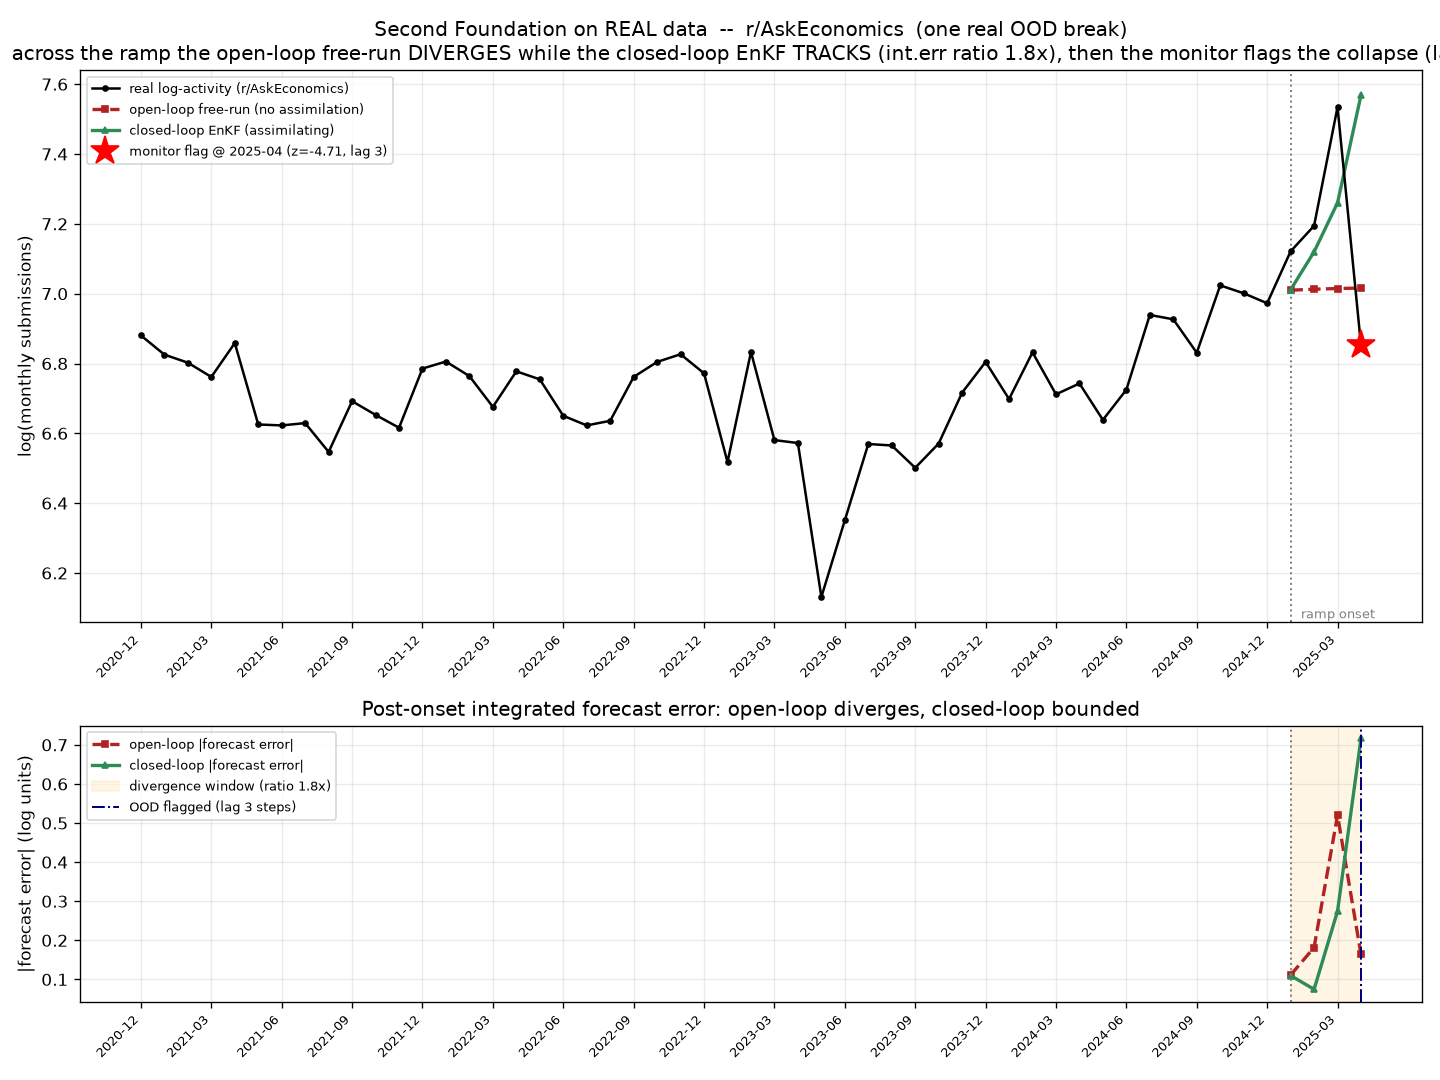
\includegraphics[width=0.92\textwidth]{validation/engine/second_foundation_realdata.png}
\caption{The Second-Foundation detect-and-correct chain on \emph{real data}: the live r/AskEconomics monthly activity series with one real out-of-distribution event (the April-2025 collapse after the Jan--Mar ramp). Across the ramp the open-loop free-run (frozen pre-onset model, no assimilation) diverges while the closed-loop EnKF assimilating each observation tracks; the misspecification monitor flags the break at the collapse (red star, $z=-4.71$) with detection lag $3$ steps and no future information. Bottom: post-onset forecast error, divergence window shaded. One block, one real event, monthly resolution; the directions (open-loop diverges, closed-loop bounded, positive detection lag) are the robust content, the magnitudes are properties of this series and the threshold.}
\label{fig:secondfoundation_real}
\end{figure}

\paragraph{Synthetic schematic.} A small companion simulation shows the same chain cleanly on a controlled synthetic low-dimensional system with an out-of-distribution jump to a unit root plus drift, where shock, noise, and threshold are all chosen rather than inherited from a real series. We report its outputs as a \emph{numerical illustration of the argument's qualitative shape}: every magnitude is a property of the chosen shock, noise, and CUSUM threshold. On a single illustrative seed the closed loop's integrated post-shock error is about $4.5$ against the open loop's about $737$, a reduction of roughly two orders of magnitude (the precise ratio varies with the draw; only its sign and order of magnitude are robust). The detection lag is $2$ steps: the monitor flags shortly after onset, never before. And as the effective number of independent model lineages $L_{\mathrm{eff}}$ (the Kish form of Eq.~\eqref{eq:kish} applied to deployed models rather than human blocks) rises from $1$ to $34$, the post-shock error falls monotonically from about $648$ to about $53$. The \emph{directions} (open-loop diverges, closed-loop bounded, error falls with $L_{\mathrm{eff}}$, lag positive) are the robust content; the numbers carry no forecast weight. The monoculture sting is the governance one: the regime that forces a single mandatory corrector ($L_{\mathrm{eff}}\to 1$) is the same regime in which human $N_{\mathrm{eff}}\to 1$ and controllability diverges (\S\ref{sec:control}), so the one indispensable controller sits on maximal leverage with minimal accountability, which is the \S\ref{sec:governance} hazard arriving by a second route. Figure~\ref{fig:secondfoundation} renders the synthetic chain: the open-loop forecast error diverging after the out-of-distribution shock while the closed detect-and-correct loop stays bounded.

\begin{figure}[t]
\centering
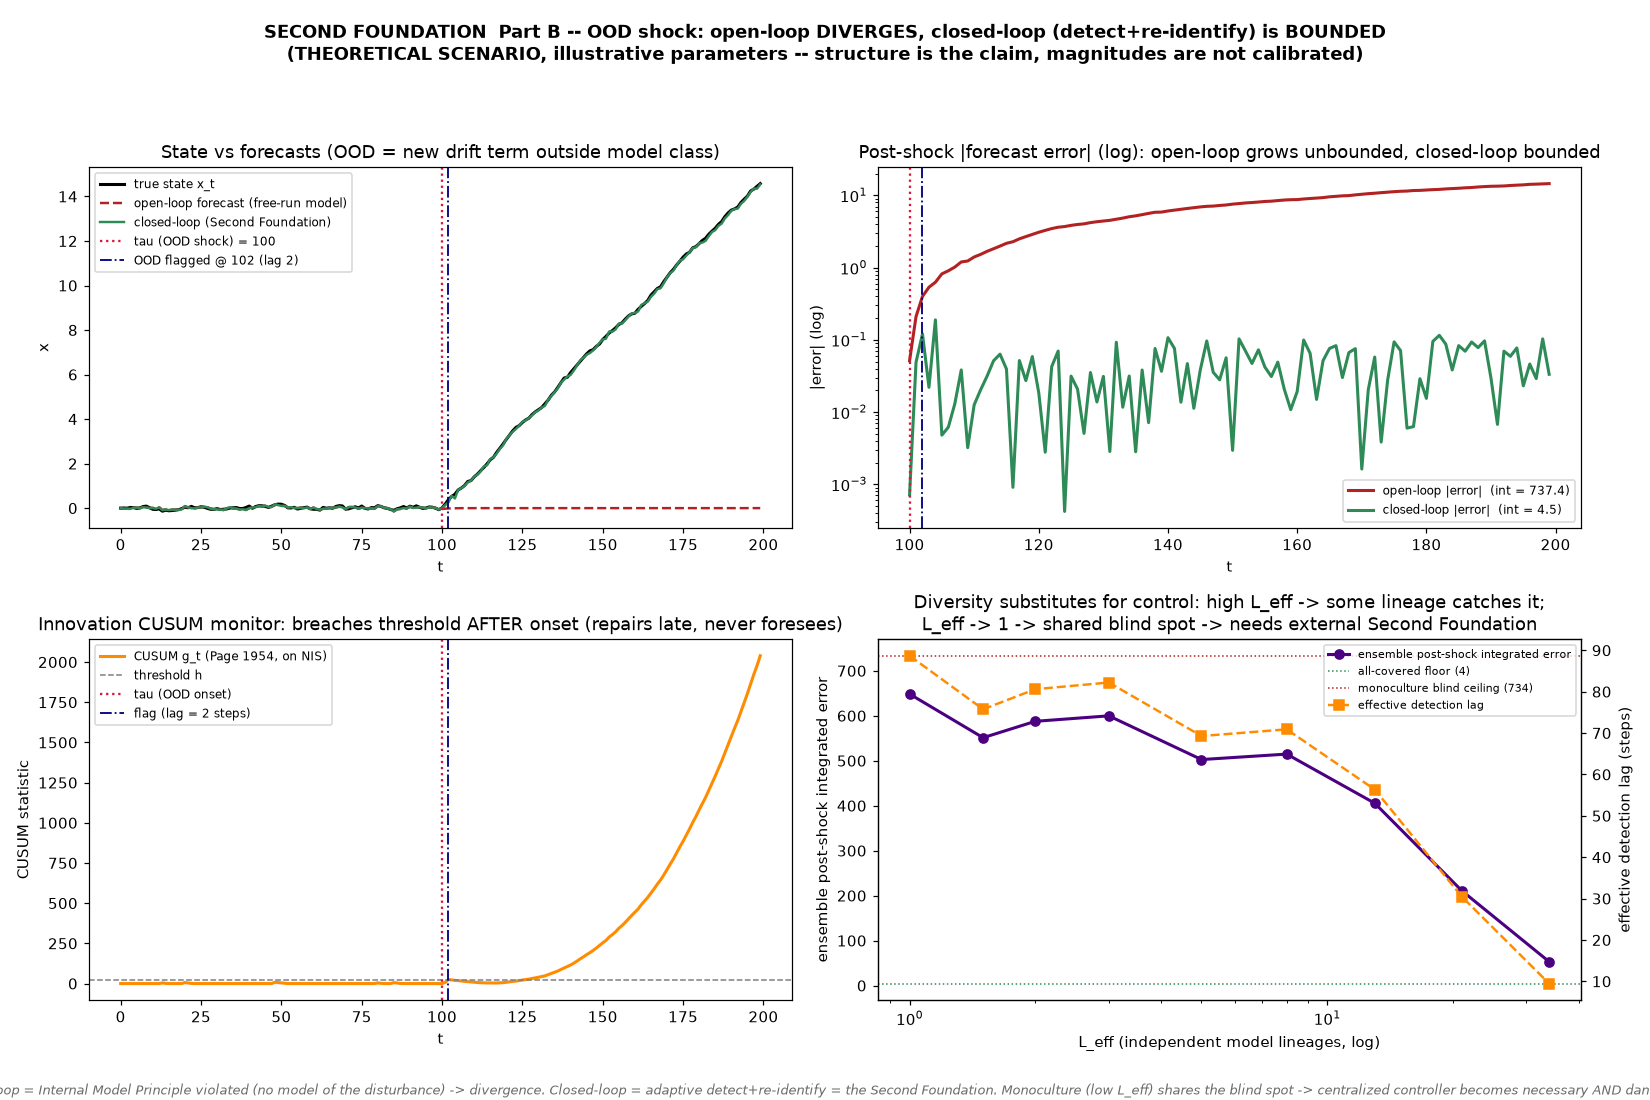
\includegraphics[width=0.92\textwidth]{validation/scenarios/second_foundation/second_foundation_sim.png}
\caption{Synthetic schematic of the Second-Foundation detect-and-correct chain on a controlled system, the clean companion to the real-data run of Fig.~\ref{fig:secondfoundation_real}: after an out-of-distribution jump (unit root plus drift), the open-loop pre-shock model's integrated error diverges while the closed adaptive loop, flagged by the CUSUM monitor a few steps after onset, stays bounded. The robust content is the directions (open-loop diverges, closed-loop bounded, positive detection lag); the magnitudes are properties of the chosen shock, noise, and threshold.}
\label{fig:secondfoundation}
\end{figure}

\section{The prediction--control duality at criticality}
\label{sec:control}

We present this section as a \emph{diagnostic and a warning}, not as a build specification. It explains why criticality is the moment of maximum manipulability, which is the reason the regime monitor must flag it; it deliberately stops short of an implementable control law, for the reasons set out in \S\ref{sec:governance}.

The repair for criticality is not better prediction. It is a change of objective. Near a critical point the static susceptibility diverges,
\begin{equation}
\chi \;\sim\; |\lambda - \lambda_c|^{-\gamma}:
\end{equation}
the static response gain to the field \emph{conjugate to the order parameter} becomes unbounded. In words, a push in just the right direction (the one the crowd is already poised to move along) produces a response that grows without bound as the system nears its tipping point, while a push in any other direction does little. This single fact has opposite signs for the two tasks. For \emph{prediction} it is fatal, since unobservable microscopic noise gets amplified to macroscopic outcomes and the branch cannot be forecast. For \emph{control} it is leverage: \emph{provided the control input couples to the critical (soft) mode} (its projection $B^\top v_{\mathrm{soft}}\neq 0$), a targeted intervention aligned with that mode gets amplified to macroscopic effect and the branch can be \emph{chosen}. The same divergence that degrades predictability maximizes this steerability-along-the-soft-mode, which we call \emph{controllability-at-criticality}. We stress that this is a linear-response (equilibrium, mean-field, quasi-stationary) statement about response gain, not the Kalman or Lie-bracket controllability rank condition: a diverging $\chi$ is necessary but not sufficient for control, since if the input has no projection on the soft mode it buys nothing. They are dual objectives on the same mechanism.

Three caveats keep the duality honest. First, the divergence amplifies only the critical (soft) mode: a generic small push is not amplified, so ``cheap control'' requires the intervention to be aligned with that mode, not merely small. Second, at the same critical point the relaxation time diverges (critical slowing-down, $\tau \sim \xi^{z}$ with $z$ the dynamic critical exponent), the very signal \S\ref{sec:criticality} uses for early warning, so the intervention that is cheap in amplitude is \emph{costly in duration}: leverage in susceptibility is paid for in commitment-time. Third, there is an internal tension to flag rather than hide: $\chi$ and the fluctuation-dissipation intuition are equilibrium constructs, while \S\ref{sec:criticality} insists critical social transitions are non-equilibrium cascades. We therefore treat the $\chi$-divergence argument as a mean-field, quasi-stationary approximation, and we note that the worked examples here are in fact \emph{basin-selection} control of a bistable system (a step intervention that permanently re-selects the equilibrium), which is a distinct and more robust control story than the linear-response one and does not require the equilibrium machinery.

The closing act of the running example is the duality made policy, and it is of the basin-selection type. On the Sunday evening of peak susceptibility, regulators issued one announcement, a guarantee costing nothing at the moment of issue, and the system-wide cascade that no model could have traced branch-by-branch was re-selected onto the no-run basin. The intervention was minimal \emph{because} the system was critical. Asimov stated this same principle narratively as the governing rule of his time-editing organization in \emph{The End of Eternity} (1955), the Minimum Necessary Change (the Eternals' own coined term) computed to yield the maximum desired effect: its operatives computed the smallest possible edit to history (a misplaced object, a single altered decision) that would propagate into the largest desired reduction in human suffering, which is precisely the claim that at criticality a minimal intervention coupled to the soft mode yields maximal leverage. We stress that minimal-in-amplitude does not mean minimal-in-consequence: the same minimality is what makes covert capture cheap, and the legitimacy of this specific intervention rests entirely on the accountability structure of \S\ref{sec:governance}, not on its cheapness (see the efficient-capture caution there). The same announcement a month earlier (sub-critical, low susceptibility) or a week later (cascade complete) would have bought far less per unit of commitment.

\paragraph{Butterflies at criticality.} This reconciles an apparent contradiction the paper has so far left standing. The block reduction of \S\ref{sec:blocks} holds that individuals are statistically negligible, averaged out by the law of large numbers over blocks; yet the common reading of history is that a few key people changed it. Both are true, in different phases. In the smooth regime the statistics are operator-independent and the lone actor washes out, which is why \S\ref{sec:blocks} can model communities rather than persons. At a critical branch point the susceptibility diverges (the $\chi$ above), so one operator's minimal choice, coupled to the soft mode, selects a branch that then propagates over long timescales. The operator exercises leverage exactly where the statistics fall silent. People can therefore have butterfly effects over long horizons by acting at criticality, without violating the statistical law that governs the smooth regime: the two claims occupy the two phases either side of $\lambda_c$, and neither refutes the other. This is also why Seldon's Plan was never pure impersonal statistics in \emph{execution}, only in its smooth-regime bookkeeping. It was steered, at its branch points, by skilled operators applying control inputs \cite{asimov1951}: Salvor Hardin manufacturing the ``religion of science'' to control the Four Kingdoms in the early Foundation, Hober Mallow's economic leverage among the Merchant Princes, and the Second Foundation's mentalics continuously nudging the trajectory back onto the Plan. Each is an operator choosing where to push, and the operator's skill is the hidden variable in the Plan's execution that the impersonal-statistics reading omits.

This motivates a regime-switching architecture. The Critical row is stated as a flagged hazard (the regime in which the population is maximally steerable, hence maximally vulnerable), not as an offered capability:
\begin{center}
\begin{tabular}{@{}lll@{}}
\toprule
\textbf{Regime} & \textbf{Diagnostic} & \textbf{Mode} \\
\midrule
Smooth & low cross-block synchrony & open-loop prediction (MFG fixed points, block statistics) \\
Pre-critical & rising synchrony, slowing-down & early warning; forecast the transition, not the branch \\
Critical & $\xi$, $\chi$ diverging & maximal manipulability (hazard flag); control only under \S\ref{sec:governance} conditions \\
\bottomrule
\end{tabular}
\end{center}
The Second Foundation, in this reading, is not a forecasting agency. It is the control layer of this architecture, exploiting criticality rather than predicting through it, and it is exactly the unaccountable power the later novels, \emph{Foundation's Edge} (1982) above all, turn against the controllers themselves. The Seldon trial is the information-release component of the control law. What the controller publishes is itself a control input, and only fixed points are safe to publish.

\section{Governance and responsible disclosure}
\label{sec:governance}

The duality of \S\ref{sec:control} is, read adversarially, the theory of operation of low-cost population steering. We hold that ``who holds the controller'' is, in the authors' own words, a design constraint of the same rank as any equation here, and we therefore give it the page budget that rank demands rather than discharging it in a single paragraph. The capability and its mitigations must travel together.

\paragraph{Defensive and offensive split.} We distinguish, and treat asymmetrically, two layers. The \emph{defensive} layer is early warning and monitoring: the state-space engine, the EnKF, the regime monitor, the misspecification flag, and the skill horizon. It is broadly useful, including to the populations being modeled, and we specify it to operational depth and endorse publishing it in full. The \emph{offensive} layer is critical-regime control synthesis: an optimal-intervention solver and a message-selection objective that targets susceptible blocks at peak susceptibility. We deliberately do \emph{not} provide its operationalization. The asymmetry is the reason: the early-warning capability is defensively useful to many parties and offensively useful to few, whereas the control capability is the reverse. Accordingly, \S\ref{sec:control} is framed as a hazard flag and a diagnostic, not as a regime-switching recipe with a control law. The mathematics does not distinguish the benign deposit guarantee from a manufactured stampede; only the objective function does, and the objective cannot validate itself (below). Where a sign must be chosen, we endorse the \emph{defensive} one: interventions that increase a population's effective number of independent units and its information (widening the branch set, buying time for deliberation, restoring its own decision-making capacity) over those that narrow the branch set to one the controller prefers. A guarantee that lets depositors stop panicking and think is defensive; a message that stampedes them is offensive. We make this a pre-action sign test rather than a sentiment, wiring it to the meter the regime monitor already computes: an intervention is \emph{defensive} iff it is projected to raise $N_{\mathrm{eff}}$ (Eq.~\eqref{eq:kish}) and lower the synchrony $r$ toward the decoupled regime, and \emph{offensive} iff it lowers $N_{\mathrm{eff}}$ or drives $r$ toward synchrony. We also state honestly what is and is not withheld: the basin-selection primitive of \S\ref{sec:control} (a step intervention that permanently re-selects the equilibrium, the SVB guarantee being the worked case) \emph{is} specified to operational depth, and it is sign-agnostic, the same mechanism serving the benign guarantee and the manufactured stampede. The paper's restraint therefore rests not on withholding that mechanism (which would be dishonest, since it is shown) but on the objective conditions (a)--(d) and the sign test above; what we decline to specify is the optimal-intervention solver and the message-selection objective that choose \emph{which} fixed point to drive a population toward. Same lever, opposite sign; the safeguard is the objective, not the secrecy. We add, in light of the empirical operator-detector (\S\ref{sec:empirical}, pilot 3), one component whose asymmetry does \emph{not} run defensive-dominant: major-player-buildup detection. The enumeration of the defensive layer above was written for an engine that reads \emph{blocks}; the operator-detector reads a single named individual building a position, which is operator-locating, not block-monitoring, and locating the individual who is about to move a crowd is symmetrically useful to a defender warning a population and to an attacker selecting a target for suppression or co-option. The asymmetry rule (defensively useful to many, offensively useful to few) fails for an operator-locator, so we pull it out of the publish-in-full defensive bucket exactly as the belief-closure simulator was pulled out below: it is published only at the aggregate, mechanism-classifier grain (gradual-internal-buildup versus sudden-external-shock) and never as a named-individual identifier or a pre-onset alarm against a specific person. The sign test above governs interventions, which change $N_{\mathrm{eff}}$; a detection capability produces no $N_{\mathrm{eff}}$ change by itself and so escapes that test, which is precisely why detection capabilities must be governed at the disclosure and access layer instead: an operator-detector is defensive when its output is a population-facing warning that raises the population's own $N_{\mathrm{eff}}$ (people learn an operator is active) and offensive when its output is a private target list that lowers it. The same signal, opposite sign, decided by who receives the output. We re-examine the adequacy of the split in this light: the demonstration that an operator-buildup detector works on real data shows a manipulator-relevant primitive (target location) is reachable from the defensive layer alone, so ``withhold the control solver'' is necessary but no longer sufficient. We concede no disclosure boundary fully closes this gap, since target location is intrinsic to early warning, and we name it as a residual exposure rather than pretend the withholding still suffices.

\paragraph{Why publish the detector at all (the net-defensive case).} Conceding a residual exposure invites the converse question, and honesty requires we answer it rather than leave the disclosure to inertia: given that exposure, why publish the operator-detector at the aggregate grain instead of withholding it alongside the control solver. We give three affirmative reasons, and claim only what they support. First, the detector is assembled entirely from standard concentration statistics (HHI, Gini, top-quantile share) applied to public participation counts; it discloses no novel primitive, and a resourced offensive actor re-derives it in an afternoon, so withholding raises the barrier for a moderator, a journalist, or a targeted population far more than for a state or a platform. This is the security field's full-disclosure argument: secrecy of a method protects mainly the defender who could least afford to lack it, while the capable attacker is undeterred. Second, the dangerous configuration of a detector is not its existence but its \emph{concentration}; a privately held operator-locator whose output is a target list is the offensive case, and the corrective is not to suppress the method but to disclose it widely enough that the population it concerns can run it on its own behalf, which raises that population's effective number of independent units (people learn an operator is active) rather than lowering it, exactly the sign of the defensive intervention above. A detector everyone can run is a worse weapon and a better shield than one only a few hold. Third, the published artifact is deliberately held to the mechanism-classifier grain (gradual-internal-buildup versus sudden-external-shock, aggregate concentration against a baseline) and withholds the per-individual scoring a prospective targeting use would require, so what we publish is the half of the capability whose asymmetry we can defend and what we withhold is the half we cannot. None of this dissolves the residual exposure named above. It states why, that exposure granted, open publication of the aggregate detector is the less dangerous of the two available configurations, which is the most any dual-use disclosure can honestly claim, and why we judge the net balance defensive rather than asserting it.

\paragraph{Conditions of legitimate operation.} We name binding minimum conditions, and declare that any deployment lacking them is illegitimate by this paper's own standard. (a) The controller's objective function must be externally authored and externally revisable, never self-authored: this is the Galaxia external-chooser point of \S\ref{sec:mule}, promoted from observation to rule. To forbid the obvious evasion (a captive ethics board that rubber-stamps an objective the controller drafted), the external author must be constituted before deployment and independently of the controller, able to revise the objective during operation and not only at commissioning, and accountable to the population acted upon. Where the forward model is a pretrained world model or reasoner (\S\ref{sec:instantiation}), the objective embedded in its prior must be treated as part of the objective function for purposes of this condition, hence externally auditable; an objective laundered through model weights satisfies (a) only nominally. (b) Every critical-regime intervention must be logged to a record the controlled population can audit; the \emph{existence} of an intervention (not its sealed contents) must be disclosed contemporaneously, exactly the Seldon-trial structure, and the disclosure lag for the contents must be bounded to the timescale of the intervention's reversibility, since an audit permitted only after the branch is permanent is a monument, not a brake. (c) No single agent may hold both the regime monitor and the control input: the seer must be separated from the hand, the oldest safeguard there is. Auditability of a single unified harness (\S\ref{sec:instantiation}) does not satisfy (c); a compliant deployment must run the regime-monitor harness and any control harness as separately operated systems with separate authority, even when both are built from the same components, because determinism makes the split inspectable but does not constitute it. (d) Where the intervention window is shorter than the external author's revision cycle, the legitimate move is a pre-authorized standing rule (a published reaction function, the lender-of-last-resort model), not real-time discretionary control: discretionary action at criticality, even with a nominal external author, fails the alignment-at-criticality limit below because the check cannot complete inside the window. A controller satisfying none of these is not performing ``minimal intervention''; it is performing efficient capture.

\paragraph{Alignment at criticality (a named limit).} The moment of maximal controllability is the moment of minimal legitimacy. At the critical point the controller's small push selects the branch, hence its \emph{objective function} selects the population's future, precisely when the population's own corrective feedback (consent, dissent, deliberation) is weakest, because consent and correction are themselves casualties of the diverging correlation length. An objective that cannot be checked by those it acts upon, at the one moment it matters most, is not safe regardless of its content. This forces the conclusion that the objective-chooser must sit \emph{outside} the machine. It is why Asimov gave the final choice to a human and not to the Plan.

\paragraph{The block is not the unit of moral concern.} The framework's natural unit is the block; a person enters only as a membership vector, a $\pi_i$-weighted mixture. That is correct mathematics and, left unqualified, dangerous ethics, because a being treated only as a mixture of blocks has no standing the controller is obliged to respect. We state plainly that the block is not the unit of moral concern (the individual is), and that any cost-benefit reckoning of an intervention must price the harm to the dissenting minority and the out-of-distribution individual \emph{separately}, never net them into an aggregate. This rule needs a ledger column to be written into, since the engine state $\Xi_t$ carries no object at the grain of the dissenting individual: we designate the misspecification monitor of \S\ref{sec:engine} as that register, and require its persistent-innovation signal to be surfaced to the objective-author as a distinct cost channel, never folded into the predictive-skill score. The instantiation of \S\ref{sec:instantiation} sharpens this obligation rather than discharging it: a block-conditioned ensemble of reasoners systematically under-represents exactly the dissenting minority and the out-of-distribution individual, since those are off-distribution by construction, so an instantiated engine must price minority and out-of-distribution harm by an external channel and never read it off the ensemble's own block-agents. A suppressed cascade is sometimes a suppressed correction; a halted run sometimes a protected fraud. The framework optimizes aggregate predictability and stability, which is not the same as human welfare and can oppose it; the choice of objective is exogenous to the machine and is the entire ethical content. The empirical operator-detector (\S\ref{sec:empirical}, pilot 3) introduces the inverse hazard to this netting problem: where the block reduction risked rendering the individual invisible, the operator-locator risks rendering a specific individual too \emph{visible}, fingerprinting the organizer or dissident this rule is meant to protect (and the out-of-distribution individual and the operator are often the same person, the Mule being the operator who moves the crowd). The rule therefore binds in both directions: the individual may be neither silently netted into a block aggregate nor singled out by a buildup signal for action that conditions (a)--(d) would forbid against the population as a whole. The Mule was a person, and so was the lone fan who stood up in the stadium. Asimov dramatized exactly this block-versus-individual tradeoff in ``The Evitable Conflict'' (1950), where the economy-managing Machines deliberately accept small, traceable harms to particular individuals (a career derailed, a firm ruined) as the price of protecting humanity in the aggregate, which is the aggregation move this paragraph forbids the controller to net silently: the harm to the individual is real even when the block-level books balance.

\paragraph{The operator has a belief vector too, and the engine shapes it.} The framework models the population's belief fields $b_k$ but carries no term for the belief of the \emph{operator} who reads the engine and chooses interventions. Two distinct facts follow, and the second does not reduce to the first. The first is a modelling gap: the operator's own $b$ is simply absent from the state, so the engine has no fixed-point condition for the observer the way \S\ref{sec:reflexivity} has one for the population. The second is influence: the engine's outputs are evidence the operator conditions on, so a reading that renders the existing community legible and an exogenous newcomer inflow invisible (the structural blind spot measured in \S\ref{sec:neffcollapse}) tends to bias the operator's own working model toward the trackable blocks. This is a \emph{second-order} reflexivity the population-level treatment of \S\ref{sec:reflexivity} does not cover: there the population conditions on the published forecast; here the seer is changed by the seeing. In this light conditions (a)--(d), which place the objective-chooser outside the machine, name a \emph{regulative ideal} rather than an achieved fact: an operator embedded in the attention economy the engine models cannot be fully external to it, so externality is something the governance regime must continually enforce, not a property it may assume. The danger is sharpened by the inverse hazard already named above: the same instrument that biases the operator to \emph{under}-see the out-of-distribution individual she is obliged to protect is, run as the operator-detector of \S\ref{sec:empirical}, exactly what can make that individual \emph{hyper}-visible as a target. We therefore name a duty rather than impute a psychology: the operator must treat the engine's legibility profile as a property of the instrument rather than of the world, and price the systematic under-weighting of out-of-distribution individuals through an external channel (the misspecification monitor of \S\ref{sec:engine}, surfaced as a distinct cost rather than folded into the skill score). An instrument that cannot register an agent will not, unaided, prompt its operator to look for one.

\paragraph{Who holds the controller, answered with mechanisms.} The running example already contains the answer the paper should state outright: the Sunday guarantee was legitimate \emph{because} it came from a chartered, mandated, ex-post auditable public body with a published reaction function and legislative review, not because the mathematics was sound. A private actor running the identical math, with a self-authored objective and no audit, would be performing the same operation illegitimately and faces none of those constraints. We do not rank the danger by actor \emph{type}, however: a captured central bank or regulator, or a state colluding with the platform that holds the attention data, can satisfy every condition (a)--(d) on paper while running the offensive operation, and the worst historical controllers held legitimate charters. The invariant is the danger scaling with the \emph{concentration} of the monitor and the control input in one locus accountable to no one, whether that locus is private, public, or a public-private fusion, which is exactly why condition (c) separates the two functions. The operator-dependence of \S\ref{sec:control} sharpens this further: the danger is not an autonomous machine but concentrated skilled operators, since the half of the engine that works now is the control half and it lives in the operator. Observer-dependence, the awareness asymmetry of \S\ref{sec:instantiation}, and criticality leverage together are the acute form of the dual-use risk, because a few aware operators acting at critical points have outsized, long-horizon, and hard-to-attribute effects. Concretely, the accountability mechanisms we point to (proposed, not endorsed as sufficient) are the lender-of-last-resort model (legal mandate, published reaction function, ex-post legislative audit), separation of monitor from controller, and disclosability of every criticality-mode intervention. The offensive analogues that share the duality's theory of operation must be named so the abstraction cannot launder them: coordinated inauthentic behavior and influence operations, recommender-system attention steering as a deployed-at-scale instance of strategic $b^{\mathrm{strat}}$, crisis-timed propaganda as control-at-criticality, and, newly demonstrated as buildable in \S\ref{sec:empirical}, pre-emptive identification and neutralization of an individual operator on the strength of a buildup signal alone, before any action, which is the pre-crime structure that condition (b)'s contemporaneous-disclosure requirement and the moral-concern rule (the individual, not the block, is the unit) are meant to forbid: a buildup flag is a warning to a population, never a warrant against a person. Absent the conditions above, the same math is an attack.

\paragraph{The trilemma is a reason to stop, not a frontier to push.} The total-observability limit (\S\ref{sec:limits}) is the technical name for total surveillance, and ``surrendering agent independence'' is the technical name for the abolition of pluralism, with real costs (chilling effects, a single point of capture, irreversibility once built). We do not aestheticize it. The trilemma is a reason to \emph{accept} bounded predictability as a design goal, and to treat the unpredictable residue as a feature that protects pluralism, not a defect to engineer away.

\paragraph{Disclosure posture for this paper.} This manuscript was drafted with AI assistance, and a dual-use review (the present section) was applied to the draft, which is why the control content is held to diagnostic depth and the control-synthesis layer is withheld. We note that \S\ref{sec:instantiation} demonstrates the machinery is assemblable from commodity components, which lowers the build barrier and therefore raises, not lowers, the burden on this posture; accordingly the instantiation there is deliberately a component mapping and an executability demonstration, and contains no control-synthesis objective, no susceptible-block targeting rule, and no message-selection step. The companion artifact is governed by the same split: its classification and per-block-reading layers are the publishable defensive component, and any objective-driven fixed-point-selection step is withheld under the conditions above. The reanalysis-corpus call of \S\ref{sec:engine} is issued as defensive-monitoring infrastructure under governance, not as an open invitation to whoever holds the most attention data (today, platforms and states, exactly the non-negligible-measure actors the paper warns about); because that corpus is itself the offensive prerequisite, possession of block-level attention history is a controller precursor and must be held under the same monitor-versus-hand separation as the controller, its construction logged as an auditable act, and possession without those audit conditions is itself illegitimate by this paper's standard. The threat model is explicit: a well-resourced actor with population-scale attention data, or a modestly-resourced actor exploiting the commodity instantiation of \S\ref{sec:instantiation} against a narrower slice of attention data, in either case with a self-authored objective and no audit, acting on a population at criticality. We commit to the asymmetry principle, discharged item by item against the \S\ref{sec:instantiation} component map: five of the six mapped components (world model, embedding clustering, perturbed-ensemble skill horizon, continual re-anchoring, deterministic harness) are defensive-dominant, while the belief-closure simulator (the fixed-point iteration over block-conditioned agents) is the one offensive-dominant component, since it is exactly the prediction-to-reaction simulator a manipulator needs to test which message switches a cascade; we therefore describe its interface (iterate to a fixed point) but withhold any objective selecting which fixed point to drive a population toward. The empirical operator-detector of \S\ref{sec:empirical} (pilot 3) is the one place this manuscript demonstrates an offensive-adjacent primitive on real, named-individual data, run retrospectively on a public, already-resolved episode and a self-identified public individual rather than prospectively against a live organizer; we publish only the mechanism-classifier verdict and the aggregate ramp-duration statistic, withhold any per-individual scoring threshold tuned to identify a specific person pre-onset, and provide none of the per-individual calibration a prospective targeting use would require. The artifacts that section produced (the labeled event rosters, the per-block mention-density series, and the operator-buildup signal traces, including those for named individuals) are themselves controller-precursor data under the standard of this paragraph: we therefore release only the aggregate, mechanism-classifier-level results and the code that computes them, withhold any per-individual buildup series tuned to identify a specific person, and hold the underlying harvest under the same monitor-versus-hand separation and auditable-construction conditions we require of the reanalysis corpus. A demonstrated detector and its validation data are not exempt from the custody rules the paper sets for the corpus; they are the first instance of them. We further note that the modern instantiation is built from the same class of language and reasoning models as one of this paper's authors, and we treat that proximity as a reason for more conservative disclosure of the control layer, not less. Finally, the falsification criteria of \S\ref{sec:limits} bear on whether the program is \emph{correct}, not on whether it is \emph{safe to deploy}: a confirmed program raises the governance stakes rather than lowering them, and scientific validation must never be read as having discharged the dual-use concern.

\section{Implementation sketch (v0)}
\label{sec:implementation}

The transplant from NWP is methodological, not physical. The operational lessons of Earth-2-class systems \cite{pathak2022}: never free-run; assimilate observations on a fast cycle; run ensembles; forecast distributions, not points; score everything.

\begin{enumerate}[label=\textbf{L\arabic*.},itemsep=2pt]
\item \textbf{Macro layer.} Stock-and-flow models for slow conserved or quasi-conserved variables (demographics, debt, energy, attention supply), in the system-dynamics tradition \cite{forrester1961,sterman2000} (with the management-practice exposition of \cite{larson} as motivation). These are reliable for claims of the form ``flows at rate $x$ with attrition $y$ imply stock $z$ in two quarters'' and silent on individuals. The social analogue of climatology rather than weather. Figure~\ref{fig:lethain_attention} shows the minimal realization of this layer: a two-stock attention model run in the lethain \texttt{systems} library, in which attention reallocates from many topics onto one while the total stays flat. The same L1 stock-flow layer was applied to $88$ real r/AskEconomics questions in a comment-concordance study (the per-post stock-flow reading scored against the actual vetted expert answer on each thread), so the schematic illustrates a layer with real application rather than a purely decorative cartoon.
\item \textbf{Block layer.} Community detection on interaction graphs to estimate blocks $B_k$ and membership vectors $\pi_i$. Per-block attention densities $\rho_k$ and belief fields $b_k$ estimated from platform, survey, mobility, and market data.
\item \textbf{Game layer.} Multi-population MFG calibrated to the block layer. The equilibrium set is computed, and published forecasts are restricted to fixed points.
\item \textbf{Assimilation.} Daily or faster re-anchoring of all layers to observations, in direct analogy to NWP data assimilation. The model is never trusted beyond its assimilation window.
\item \textbf{Ensembles and scoring.} Perturbed-initial-condition and perturbed-parameter ensembles. Outputs as distributions scored by Brier/CRPS against resolution \cite{tetlock2015}. The baselines to beat are existing superforecasting aggregates and incentive-compatible market-implied probabilities (prediction markets, and for the SVB-type case fed-funds futures and credit-default-swap spreads), scored where they exist. We state the baseline honestly: the skill of curated geopolitical-tournament forecasting is real but selected (the questions were chosen to be resolvable and non-trivial) and decays sharply beyond roughly three to six months, so it is evidence that \emph{some} smooth-regime tasks are tractable for \emph{other} methods, not an existence proof that this engine works, which is untested.
\item \textbf{Regime monitor.} Continuous estimation of cross-block synchrony, variance, and autocorrelation as early-warning indicators \cite{scheffer2009}. The published product includes the system's own current predictability as a first-class output.
\end{enumerate}

\begin{figure}[t]
\centering
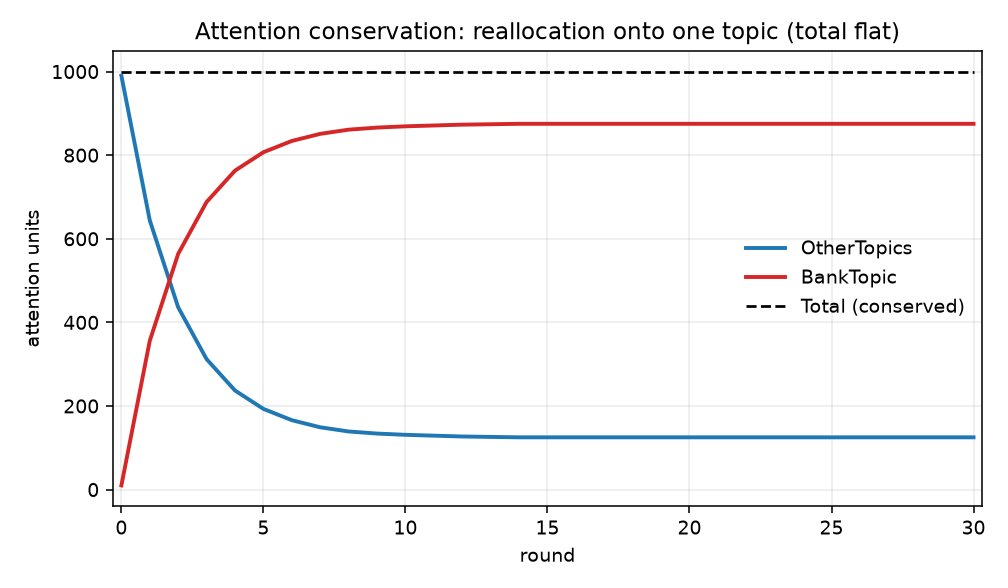
\includegraphics[width=0.72\textwidth]{figures/lethain_attention.png}
\caption{A lethain stock-and-flow run of the macro layer (L1): total attention is conserved while it reallocates from many other topics onto a single bank topic (the leak rate onto the bank topic exceeds the return leak, so the bank topic fills until the back-flow balances it). The dashed total stays flat to the unit, illustrating the slow-stock, budget-constrained layer of \S\ref{sec:attention} in the smallest possible model. An illustrative synthetic stock-flow demonstrating the conserved-reallocation shape.}
\label{fig:lethain_attention}
\end{figure}

We make L1--L6 a \emph{staged} program with an explicit gate, honoring the split of \S\ref{sec:governance}. The prediction-and-early-warning stack (L1--L6) is the publishable, buildable, auditable artifact, and it is what an implementer can start on: the macro layer (L1) and a community-detection prototype (L2) are tractable on real data today, while the fast, belief, and assimilation core awaits the corpus, the topic-graph instantiation, and the observation operator of \S\ref{sec:engine}. The closed-loop critical-regime controller is \emph{not} specified operationally here and is gated behind the conditions of \S\ref{sec:governance}: we provide enough to build the monitor and deliberately not enough to build the manipulator.

\section{A modern instantiation: world models and ensembles of reasoners}
\label{sec:instantiation}

The engine of \S\ref{sec:engine} was specified abstractly: a forward model, an observation operator, an ensemble assimilation cycle, a mean-field-game belief closure, and a skill horizon. We left several of its components as open specification points, and the constitutive problem of \S\ref{sec:attention} in particular was relocated rather than solved. The purpose of this section is a narrow existence argument, kept inside the paper's own hedges. We claim that, as of the mid-2020s, each abstract component has at least one concrete realization assembled from off-the-shelf artificial-intelligence parts, so that the binding constraint on a bounded psychohistory is no longer the \emph{existence of the machinery}. The binding constraint is, exactly and only, the two structural conditions the paper has already isolated: a smooth (monotone, sub-critical) regime, and an audience that is either unaware of the forecast or, if aware, conditioned on a published fixed point. This is an argument about instantiability: it demonstrates that the loop can be \emph{built and run}, with the distinct question of whether the loop \emph{forecasts} reserved for the scored tests of \S\ref{sec:limits}.

\subsection{Component mapping}

We map each abstract component of \S\ref{sec:engine} to a modern realization. The arrow reads ``is realized by.''
\begin{itemize}[itemsep=3pt,leftmargin=1.4em]
\item \textbf{Forward / world model $\mathcal{M}$ $\rightarrow$ a large pretrained world model.} A large pretrained world model is a model that has learned, from a vast record of behavior, an internal simulator of how things tend to respond to what is done to them. Such a model supplies a learned prior over how blocks respond to stimuli, and that prior is precisely the constitutive law for the belief drift field $b$ that the constitutive problem of \S\ref{sec:attention} left open. This is the social analogue of the learned weather surrogate that motivated the program (the FourCastNet and Earth-2 substitution of a learned operator for an integrated physics \cite{pathak2022}), built on the same attention substrate \cite{vaswani2017}, and of the world-model construction in the reinforcement-learning sense \cite{ha2018}. We are careful about what this is: a \emph{prior} over responses, a learned distribution, not a closed-form constitutive law and not a guarantee of calibration. It stands to the social problem as the weather surrogate stands to the atmosphere, with the decisive difference that no \emph{open} social reanalysis corpus (\S\ref{sec:engine}) yet exists to ground it. The raw material does exist: IRC logs, Reddit and its archives, the Internet Archive and the Wayback Machine, platform engagement and view logs, and video view histories are the recorded digital history this engine would assimilate, and proprietary corpora of exactly this kind are already held and experimented on at population scale by closed actors. The Facebook emotional-contagion experiment, which manipulated the news feeds of $689{,}003$ users \cite{kramer2014}, is at once proof that such a corpus exists privately and an instance of the population-scale control \S\ref{sec:governance} warns about. The missing thing is therefore not the data but \emph{open, accountable access} to it, and the actors who already hold it are the unaccountable controllers of \S\ref{sec:governance} rather than a separate party. This is, in the canon's terms, a Prime Radiant learned from data rather than authored by Seldon, and it inherits the same hazard: whoever may edit the model holds the population. It is also Asimov's own image of the centralized predictive social engine, his recurring supercomputer Multivac, rebuilt in distributed form: where Multivac was a single oracle, the world-model-plus-ensemble of this section is a Multivac smeared across many components. Multivac is the right ancestor precisely because Asimov used the one machine for all three of this paper's architectures across these stories: an oracle in ``Franchise,'' a standing controller in ``The Evitable Conflict,'' and a total-surveillance predictor in ``All the Troubles of the World'' (\S\ref{sec:limits}), which are prediction, control, and total observability in a single fictional lineage.\footnote{In ``Franchise'' (1955) Multivac forecasts an entire national election not by extrapolating one representative voter's opinions but by interrogating the single citizen whose few remaining answers supply the last bits of information it lacks, having already absorbed the rest of the electorate as data; the voter is the one residual degree of freedom, not a representative sample, which is the soft-mode point of \S\ref{sec:control} (at a critical branch a single residual perturbation, not the bulk statistics, decides the outcome) and a cautionary case for \S\ref{sec:blocks}, since it drives the effective number of independent units (Eq.~\eqref{eq:kish}) toward one. The ``Machines'' of ``The Evitable Conflict'' (1950), the closing story of \emph{I, Robot} (1950) and the capstone of the Machines arc, are the complementary image: positronic computers that quietly run the world economy as a standing, mature feedback controller, making small continuous corrections and tolerating minor harm to individuals to protect humanity in the aggregate, which is the control layer of \S\ref{sec:control} and the block-versus-individual problem of \S\ref{sec:governance} in narrative form.}
\item \textbf{Blocks $B_k$ and memberships $\Pi$ $\rightarrow$ embedding clustering plus community detection.} Embedding-based clustering of agents and topics, combined with community detection on interaction graphs, estimates the blocks $B_k$ and the mixed-membership vectors $\pi_i$ of \S\ref{sec:blocks}, the empirical realization of Simon's near-decomposability \cite{simon1962} and of the mixed-membership stochastic blockmodel \cite{airoldi2008}. This is the L2 layer of \S\ref{sec:implementation} made concrete, and it is the part already tractable on real data.
\item \textbf{MFG belief closure (Eq.~\eqref{eq:closure}) $\rightarrow$ an ensemble of language and reasoning models simulated to a fixed point.} Rather than solving the coupled HJB/Fokker--Planck system of Eq.~\eqref{eq:mfg} as a PDE, one can compute its prediction-to-reaction fixed point by iterated simulation. An ensemble of large language models (LLMs) and large reasoning models (LRMs), each conditioned to act as a block $B_k$, reads a candidate published forecast, best-responds, and the aggregate response is re-fed as the new candidate until the iteration reaches a fixed point. The reasoning models carry the multi-step best-response and the adversarial self-checks; the language models carry the per-block reading. This computes the reflexive fixed point of \S\ref{sec:reflexivity} by simulation in place of the analytic solve. It inherits that section's uniqueness caveat, with one honest correction. Strict monotonicity (Eq.~\eqref{eq:monotone}) secures \emph{uniqueness} of the equilibrium but not \emph{convergence} of an undamped best-response iteration. The simulated best-response map is an uncontrolled approximation to the monotone operator $F$, so convergence is empirical and not guaranteed by Eq.~\eqref{eq:monotone} alone. It requires the prediction-to-reaction map to be a contraction in a suitable metric, which a damped, Krasnoselskii-averaged update is used to secure. Consequently, in the imitative regime the iteration can land on different points from different seeds and prompts. That seed-dependence is only \emph{consistent with} equilibrium multiplicity, and it must be distinguished from mere solver non-convergence by checking that the distinct limits are each individually stable under further iteration. Only stable distinct limits evidence true multiplicity, so divergence alone is not a reliable diagnostic of it.
\item \textbf{Ensemble forecast and skill horizon $\tau^\ast$ $\rightarrow$ perturbed-prompt, perturbed-seed ensembles.} Perturbing prompts and sampling seeds across the LLM/LRM ensemble produces a forecast spread, the direct analogue of the perturbed-initial-condition and perturbed-parameter ensembles of \S\ref{sec:engine}. The lead time at which that spread reaches base-rate (climatological) spread is the empirical skill horizon $\tau^\ast$, with all the caveats of \S\ref{sec:engine}: it is a degradation time whose cause (genuine divergence versus coefficient breakdown) the ensemble cannot self-diagnose, and it must be emitted together with the misspecification flag.
\item \textbf{Assimilation (Eq.~\eqref{eq:enkf}) $\rightarrow$ continual re-anchoring.} Continual re-conditioning of the agents and of the low-dimensional parameters to fresh observations is the ensemble-Kalman analogue: the agents are re-anchored to current data each cycle, the model is never free-run, and the misspecification monitor (persistent irreducible innovation, degenerate rank histogram) flags out-of-model agents exactly as in \S\ref{sec:engine}.
\item \textbf{Workflow orchestration $\rightarrow$ a deterministic harness.} A deterministic workflow, meaning a fixed and inspectable recipe of steps that always runs in the same order (``harness'' is a synonym), sequences the loop classify $\rightarrow$ model-each-layer $\rightarrow$ synthesize, with adversarial verification at the synthesis step, which is the engine's prescribed cycle of \S\ref{sec:engine} restated as an executable harness. The determinism is load-bearing for governance, not cosmetic: a fixed, inspectable orchestration is what makes the ensemble \emph{auditable} (\S\ref{sec:governance}) rather than a single opaque oracle, because the routing, the per-block conditioning, and the fixed-point iteration are each separately logged.
\end{itemize}

\subsection{A reflexive existence proof, bounded}

A companion artifact to this paper makes the point concretely, and we are deliberate about how little it shows. The artifact is a small skill plus an ensemble-of-agents workflow that routes a question onto the framework's layers (conservation, blocks, reflexive fixed points, criticality, observation) and produces per-block structured readings. Run over a corpus of one hundred real economics questions, it routed roughly ninety percent of them onto at least one layer, and the criticality branch activated on a minority of questions.\footnote{The reported figure is a router coverage rate: the denominator is the questions attempted, and ``routed'' counts a question on which at least one framework layer was activated above the router's activation threshold. It is a property of the router and the question set, not a skill metric.} That minority activation is a fact about the router's thresholds and the question set, carrying no information about how often criticality occurs in the world.

We state with care what this does and does not establish, and the statement turns on a distinction the word ``skill'' otherwise hides. There are two senses of skill, and only one of them waits on the corpus. \emph{Forecast skill} is open-loop predictive accuracy scored against ground truth: how often the engine's published, pre-registered, out-of-sample forecasts come true. That is the sense that requires an \emph{open}, calibrated social reanalysis corpus (\S\ref{sec:engine}) and the scored predictions of the kind \S\ref{sec:limits} commits to; the corpus exists privately, held by the closed actors of \S\ref{sec:governance} \cite{kramer2014}, but no openly accessible one does, and nothing in this subsection bears on that sense. \emph{Operator skill} is the distinct thing: the effect a skilled observer or operator produces by using the engine to choose interventions toward an objective. Operator skill is observer-dependent and realizable now, and it does \emph{not} require accurate forecasting, because at a critical point the operator does not need the trajectory. They need to detect the susceptible moment, which the early-warning layer already provides, and apply the minimal intervention coupled to the soft mode (\S\ref{sec:control}). The skill is in the timing and target of the lever, not in forecasting which branch the crowd takes. This is the control side of the prediction--control duality: the unvalidated half is prediction, and the half that works now is control, and it lives in the operator. The same engine in different hands therefore produces different histories, because the mathematics is operator-independent in the smooth regime (it is statistics) while the application is operator-dependent at criticality (a few key people choosing where to push).

With that distinction fixed, this artifact demonstrates the \emph{executability} of the classification and per-block-reading layers by an LLM/LRM ensemble inside a deterministic workflow: the machinery runs, routes, and emits structured per-block output without human intervention. Its standing is exactly that: an existence proof of the \emph{machinery}, establishing executability, with \emph{forecast} skill reserved for the scored, out-of-sample tests of \S\ref{sec:limits}. The activation rate is a property of the router and the question set, a measurement of the pipeline rather than of how often criticality occurs in the world. This is therefore an existence proof of the \emph{machinery}, in the same spirit as the internal-consistency checks of \S\ref{sec:figures}. The contribution of this subsection is to move ``the components can be assembled'' from assertion to demonstration.

\subsection{The binding caveat: the modern stack does not repeal the two limits}

The existence of a modern instantiation changes the location of the difficulty, not its character. A bounded psychohistory built from world models and ensembles of reasoners is bounded by the \emph{same} two limits as the abstract engine, and the modern parts do not relax either one.

\paragraph{(a) Criticality is not bought off by a larger model.} At a critical transition the static susceptibility diverges ($\chi \sim |\lambda-\lambda_c|^{-\gamma}$, \S\ref{sec:control}) and the branch is selected by microscopic noise that no observation resolves. A larger world model does not help here, because the obstruction is not a deficit of model capacity or training data but the divergence of sensitivity itself: in the critical regime the coefficients calibrated in the smooth regime are simply wrong (\S\ref{sec:criticality}), and a more capable model calibrated the same way is wrong in the same way. The objective must switch, exactly as in \S\ref{sec:control}, from prediction to early warning and minimal-intervention control. Scaling the instantiation buys smooth-regime resolution and buys nothing at the transition.

\paragraph{(b) Awareness, restated for the artificial-intelligence era.} This is Asimov's secrecy axiom (O2, \S\ref{sec:objections}) and it survives the modern stack intact. The moment the population can condition on the engine's published predictions, those predictions enter the reaction map at the meta level and are self-defeating unless they are fixed points (\S\ref{sec:reflexivity}). An openly deployed, publicly known LLM-ensemble psychohistory engine alters the very distribution it models, including through the population's own models of the engine, so the predictable regime is precisely
\[
\text{smooth dynamics} \;\wedge\; \text{regime-stationary coefficients} \;\wedge\; \big(\text{secret prediction} \;\vee\; \text{self-fulfilling fixed-point publication}\big).
\]
The regime-stationary conjunct carries the Lucas exposure of \S\ref{sec:objections}: secrecy buys predictability only while the coefficients have not broken, so the ``secret prediction'' disjunct is not unconditional. Moreover the ``self-fulfilling fixed-point publication'' disjunct holds only insofar as the fixed point \emph{remains} a fixed point after the engine's own outputs re-enter the corpus the next population conditions on (the reflexive-corpus term sharpened just below). A psychohistory whose non-fixed-point forecasts are public is self-invalidating. This is Seldon's secrecy requirement re-derived, not assumed, and it is the structural reason the openly published parts of this program must be the early-warning and fixed-point layers (the defensive layer of \S\ref{sec:governance}), never the raw forecasts. The ceiling has a defensive corollary worth claiming: because an openly known engine perturbs the distribution it models, public knowledge of the engine's existence is itself a partial safeguard against its covert use, a further argument for disclosing the engine's existence and defensive layer while withholding the control objective. We do not oversell it, since the secret-deployment case (the ``secret prediction'' disjunct) still defeats it. The argument so far runs on the \emph{population's} awareness; a distinct and worse case is a \emph{hostile major player} aware of the engine. An adversary who reads the early-warning layer we endorse publishing learns exactly when the population is maximally steerable, so that defensive layer is, to such an actor, a criticality \emph{clock}: the timing information is the offensive payload of \S\ref{sec:governance} handed over by the defensive layer. We add this to the threat model rather than wave it off. One might hope that early-warning precursors are typically public, so the clock is closer to common knowledge than to a private edge; that hope does not hold for the working case. First contact (\S\ref{sec:empirical}) finds that the impersonal precursor washes out while the operator-buildup detector does the discriminating, so the clock an adversary would actually read is that operator detector, whose thirteen-week pre-onset ramp is \emph{not} a public statistic. The public-precursor hope does not survive the empirical section, and the residual is a real and larger exposure than that hope allowed.

There is a sharper symmetry, and it is the structural ceiling on the whole program rather than an incidental nuisance. An ensemble of reasoners that is \emph{itself} trained on, and aware of, psychohistory, deployed openly, is simultaneously the predictor and a perturbation to what it predicts. Its outputs are part of the corpus the next population conditions on; its public existence is part of the state it models. Such an open engine aware of psychohistory is the first Mule the Plan ever manufactured for itself: an out-of-model agent of its own making, since its outputs join the corpus and its existence joins the state. Awareness is therefore not a problem one engineers around with a better model. It is the ceiling: the modern instantiation makes the machinery real and leaves the two classical limits exactly where the paper found them.

\subsection{An illustrative application: the AI transition itself}
\label{sec:mythosfable}

We close the instantiation section by turning the engine on the very transition that makes it buildable. This subsection is deliberately a focused \emph{scenario ensemble}, not a single forecast, and we put the honesty rail first rather than last, because the temptation to read any one trajectory as a prediction is exactly what the framework forbids. We separate the parameters into two kinds. The \emph{observable} drivers (cost per token, frontier release cadence, AI attention share) are set from data and held fixed; the genuinely unknown \emph{structural} parameters (the attention-capture rate $\alpha$, the homogenization exponent $p$, the effective lineage diversity $L_{\mathrm{eff}}$, and the baseline block count $K$) are \emph{swept over plausible ranges}. What results is a range of scenarios rather than one curve. No individual date in any member of the ensemble is a prediction; the load-bearing output is the robust \emph{ordering} and the qualitative \emph{shape} of the trajectory (attention capture, then a collapse of the effective number of independent human blocks, then a phase flip), both of which hold across essentially the entire ensemble even though the dates do not. This is precisely the regime the paper says it can shape but not date.

\paragraph{The observed drivers.} Apply the engine to artificial intelligence as its own object. Three slow stocks are pinned to observed values rather than invented. First, a cost per token $\kappa$ that falls by roughly an order of magnitude per year: Epoch AI's inference-price data put the decline at a median of about $50\times$ per year to reach a fixed capability level (a $9$ to $900\times$ spread across benchmarks, with the GPT-4-level GPQA threshold falling about $40\times$ per year), so the $\sim 10\times$ per year we adopt is the deliberately \emph{conservative} anchor, since a steeper decline only accelerates the collapse. Second, a frontier capability $C$ that grows with release cadence: the median gap between frontier model releases is on the order of $50$ to $60$ days (per-lab 2025 medians of roughly $58$, $67$, and $75$ days, with an all-lab industry median nearer two weeks), a monthly-to-bi-monthly tempo that we read as a $\sim 2.5\times$ per year effective-capability trend (``capability'' is a soft composite, so this is a trend, not a measurement). Third, an AI share of human informational attention $A_{\mathrm{ai}}$ obeying $A_{\mathrm{ai}} + A_{\mathrm{human}} = 1$, initialized from a \emph{clearly-bounded plausible estimate} rather than a precise statistic: chatbot-versus-search traffic is only a few percent, but a leading assistant reporting on the order of $900$ million weekly users mediates a larger informational slice, so we take the current share to lie in the bounded range $[0.05, 0.15]$ and sweep within it, stating plainly that this is an estimate, not a measurement. That last identity is the conservation law of \S\ref{sec:attention}, exact here by construction: attention given to AI-mediated cognition is attention not given elsewhere. Capture is logistic, $\dot A_{\mathrm{ai}} = \alpha\, v\,(1-A_{\mathrm{ai}}) - \mathrm{churn}\cdot A_{\mathrm{ai}}$, with a value pull $v$ rising in capability and falling in cost: the more attention AI already holds, the more cognition routes through it. Figure~\ref{fig:lethain_ai_capture} renders the conservation backbone of this scenario as a lethain stock-flow, attention reallocating from a human stock to an AI stock under a capture leak with a small back-flow, the total held fixed by the $A_{\mathrm{ai}}+A_{\mathrm{human}}=1$ identity. It is deliberately a synthetic schematic: it carries the conserved-reallocation shape alone, while the logistic capture law, the model-lineage diversity, and the timing are developed in the rest of this subsection as scenario structure.

\begin{figure}[t]
\centering
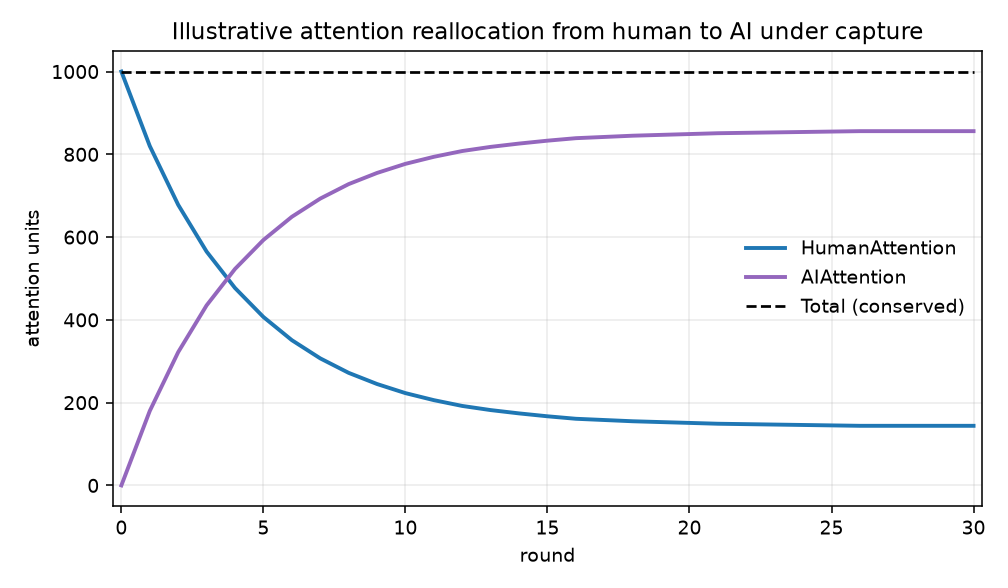
\includegraphics[width=0.72\textwidth]{figures/lethain_ai_capture.png}
\caption{Illustrative lethain stock-flow of attention reallocating from a human stock to an AI stock under a capture leak, with a small back-flow; the total is conserved (the $A_{\mathrm{ai}}+A_{\mathrm{human}}=1$ identity of \S\ref{sec:attention}). This is a clearly illustrative analogue of the mythos-fable scenario, carrying only the conserved-reallocation shape; the capture timing is a property of the chosen parameters and is read as scenario structure, not forecast.}
\label{fig:lethain_ai_capture}
\end{figure}

\paragraph{The model-layer diversity.} The payload is a diversity diagnosis. What matters is not the raw number of deployed models $M$ but the effective number of independent model \emph{lineages},
\begin{equation}
L_{\mathrm{eff}} \;=\; \frac{M}{1 + (M-1)\,\rho_{\mathrm{model}}},
\label{eq:leff}
\end{equation}
the Kish form of Eq.~\eqref{eq:kish} applied to deployed models, with $\rho_{\mathrm{model}}$ the inter-model correlation (high when models are distilled or fine-tuned from a shared base). The consequences are stark and are illustrated, not measured. A swarm of small language models distilled from one base has huge $M$ but $L_{\mathrm{eff}}\approx 1$: apparent diversity is not actual diversity, a monoculture wearing a million masks. Raising the model-to-human ratio buys no plurality if $\rho_{\mathrm{model}}$ stays high, since $L_{\mathrm{eff}}\to 1/\rho_{\mathrm{model}}$ as $M\to\infty$, so per-person agents forked from one base remain a monoculture. And the economics drives $L_{\mathrm{eff}}$ small: resource barriers (power, water, cooling, compute, and a training cost that is the real barrier to a \emph{new lineage}) keep the number of independent base lineages small and shrinking, even as falling inference cost multiplies $M$ and raises capture. A monoculture is the cost-minimizing equilibrium. Illustrative lineage figures (an oligopoly at $L_{\mathrm{eff}}\approx 1.3$, a per-tribe regime at $L_{\mathrm{eff}}\approx 18$, a million-model swarm still at $L_{\mathrm{eff}}\approx 1.03$) span the range we sweep, not measurements.

\paragraph{The swept structural parameters.} The genuinely unknown quantities are not observable, so we refuse to invent point values for them and sweep them instead. The companion ensemble (\texttt{validation/scenarios/mythos\_fable/ensemble.py}, run with \texttt{py -3.12}) crosses four structural knobs over plausible ranges: the attention-capture rate $\alpha \in \{0.15, 0.28, 0.50\}$ (low, central, high), the homogenization exponent $p \in [1,3]$, the effective lineage diversity $L_{\mathrm{eff}}$ from monoculture ($\approx 1.3$) through oligopoly ($\approx 4$) to diverse ($\approx 18$), and the baseline block count $K \in \{100, 1000, 5000\}$, with $L_{\mathrm{eff}}$ entering as a ceiling on the achievable cross-human correlation ($\rho_{\max}\!\approx\!1/L_{\mathrm{eff}}$, so diverse lineages cannot correlate the whole population even at full AI attention). The observed drivers above are held fixed throughout. Every result below is a \emph{range} over this $243$-member ensemble, never a single trajectory.

\paragraph{The phase flip.} As $A_{\mathrm{ai}}$ rises and routes cognition through few lineages, the cross-human correlation rises (modeled as $\rho \propto A_{\mathrm{ai}}^{\,p}$) and the human $N_{\mathrm{eff}}$ of Eq.~\eqref{eq:kish} collapses toward $1$. In the language of \S\ref{sec:nearcond}, the system crosses from the World Cup phase ($K<K_c$, many adversarial sub-critical blocks) into the Pluribus hive ($K>K_c$, one synchronized block). AI attention-capture is the control parameter that pushes the effective coupling past $K_c$: it is the mechanism by which premise (b) of \S\ref{sec:nearcond}, sub-criticality, the one premise the paper flagged as empirically at stake, can fail. The Kish form is brutally sensitive at large $K$, so a modest shared correlation collapses independence fast; that sensitivity is a real property of the framework (\S\ref{sec:blocks}), not a tuning artifact.

\paragraph{Structural conclusion.} Stated plainly: rising capability together with falling cost drives attention capture and a collapsing human $N_{\mathrm{eff}}$, which makes the population simultaneously \emph{less self-predictable} (susceptibility diverges, the skill horizon $\tau^\ast \to 0$, \S\ref{sec:control}) and \emph{more steerable} (frontier-agent leverage rises), with the unrestricted frontier models as the major players (\S\ref{sec:engine}) holding that leverage, and the reflexive awareness loop of \S\ref{sec:instantiation}(b) capping the horizon because the object being modeled is also the thing reading the model. This is \emph{not} a default-extinction claim. It is a loss-of-plurality claim: the headcount of humanity is unchanged, but its effective number of independent units collapses, a thousand decision-communities behaving first as a handful, then as one. A homogenized mass with diverging susceptibility is both harder to predict and easier to steer, and the steering wheel sits with whoever holds the unrestricted frontier. Loss of plurality is not only the crowd synchronizing; it has a second, faster channel that the operator-buildup detector of \S\ref{sec:empirical} just made real. The same detector that finds an operator before a cascade lets whoever holds the frontier identify and suppress the residual human operators (the organizers, the dissenting major players) who are the last sources of branch-diversity in a homogenizing population, removing the last reservoir of plurality the synchronization left standing. The targeted-suppression channel is the deliberate removal of the few who could still push a different branch, and it is enabled by this paper's own demonstrated tool.

\paragraph{How the milestones arise from the equations.} The ordering is not stipulated; it falls out of the structure. Capture is logistic in a value pull $v$ that scales as capability over cost, so as $\kappa$ falls (the observed $\sim 10\times$ per year) the pull rises and $A_{\mathrm{ai}}$ accelerates: the attention share is driven by the slow stocks, not free. Rising $A_{\mathrm{ai}}$ raises the cross-human correlation through $\rho \propto A_{\mathrm{ai}}^{\,p}$, and that correlation collapses $N_{\mathrm{eff}}$ through the Kish form $N_{\mathrm{eff}}=K/(1+(K-1)\rho)$, which at large $K$ is brutally sensitive (a correlation of order $1/K$ already halves it). The skill horizon tracks $\tau^\ast \propto N_{\mathrm{eff}}/K$, so it falls \emph{first}: homogenization bites the forecast horizon while the correlation is still small, well before the same homogenization has pushed the \emph{visible} attention share $A_{\mathrm{ai}}$ past one half. That is the mechanism behind the robust ordering, self-predictability eroding before capture is visibly dominant, and it is why the ordering survives the sweep even though the dates do not.

\paragraph{Milestone ranges across the ensemble.} The companion ensemble reports, for each milestone, a \emph{range} of crossing times over the $243$ structural settings, explicitly tagged as scenario ranges and load-bearing on nothing as individual dates. The skill horizon $\tau^\ast$ halves within roughly the first several months to about a year in the bulk of the ensemble (full spread $\approx 0.3$ to $6$ years, median $\approx 1.0$ year). The human $N_{\mathrm{eff}}$ falls below $10$ within roughly half a year to a few years in the collapsing members (spread $\approx 0.4$ to $9.6$ years, median $\approx 2.6$ years), and in the high-diversity members it never reaches that line within the decade at all, the lineage diversity preventing the collapse outright. AI crosses an attention majority within roughly two to a handful of years, occasionally longer (spread $\approx 1.8$ to $7.4$ years, median $\approx 3.3$ years). No single one of these dates is a prediction; the spreads are the point.

\paragraph{What drives fast versus slow collapse.} The sensitivity is clean and one-line per milestone. The capture rate $\alpha$ dominates the timing of the attention majority (it sets a spread of roughly five years on that milestone, by far the widest). The lineage diversity $L_{\mathrm{eff}}$ together with the homogenization exponent $p$ dominate the $N_{\mathrm{eff}}<10$ crossing: high $L_{\mathrm{eff}}$ (low $\rho_{\mathrm{model}}$) delays it and, in the diverse limit, prevents it, while steep $p$ sharpens it. The block count $K$ starts the trajectory higher but, once the coupling is super-critical, the system collapses on a similar schedule regardless, so $K$ moves the $\tau^\ast$-halving date most but the later milestones least. Stated as a rule: high capture $\alpha$ and high homogenization $p$ accelerate the collapse; high lineage diversity $L_{\mathrm{eff}}$ (equivalently low inter-model correlation $\rho_{\mathrm{model}}$) delays it or, in the limit, prevents it; a larger $K$ starts higher but collapses similarly once coupling is super-critical.

\begin{figure}[t]
\centering
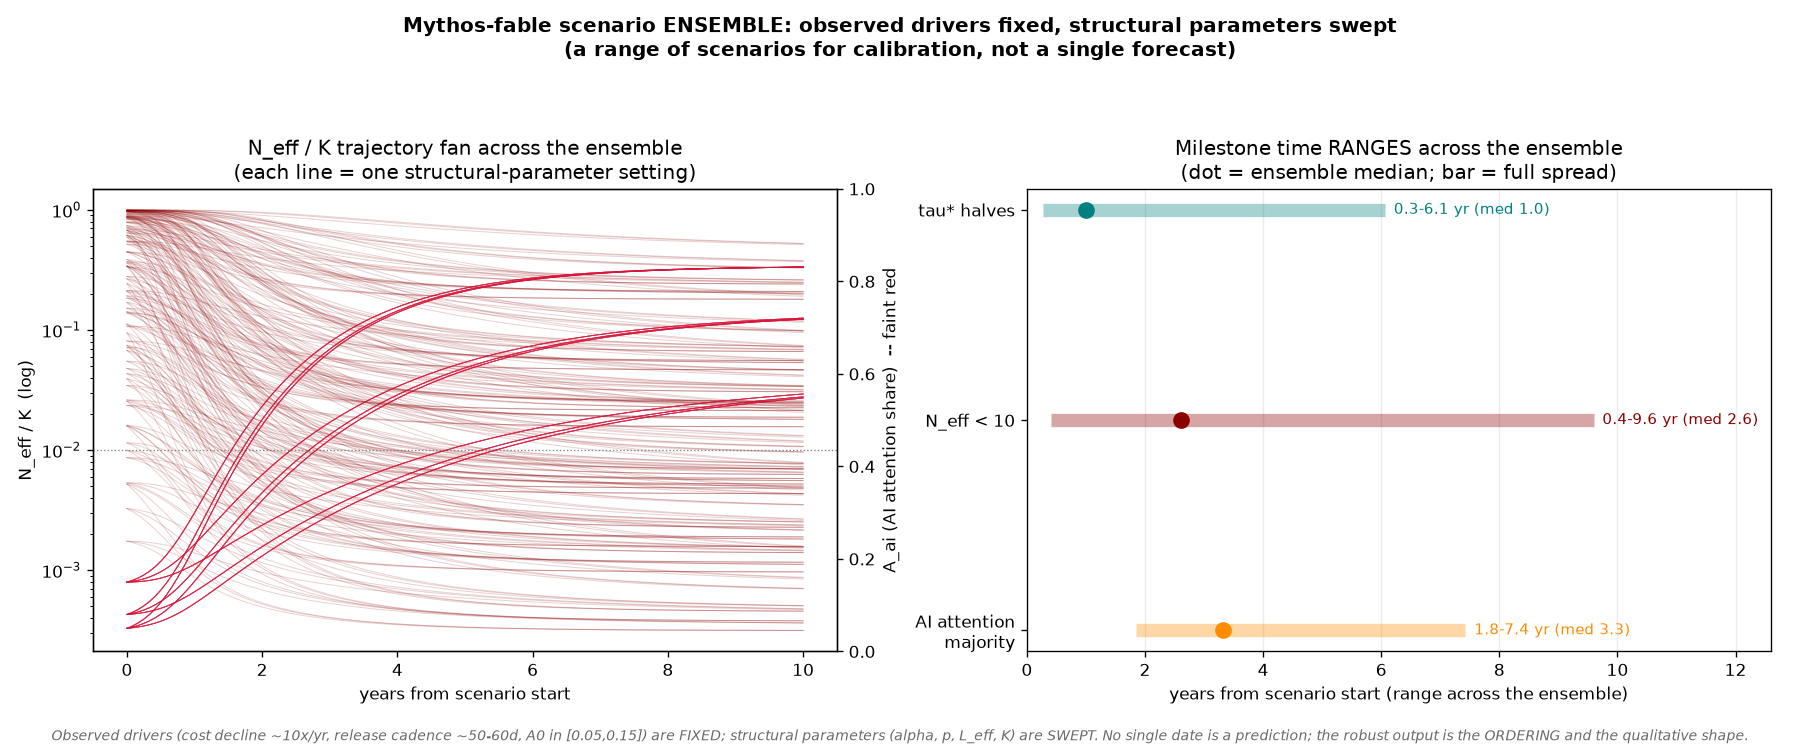
\includegraphics[width=0.95\textwidth]{figures/mythos_fable_ensemble.png}
\caption{The mythos-fable scenario \emph{ensemble}. Left: the fan of $N_{\mathrm{eff}}/K$ trajectories (dark) and AI attention shares (faint red) across all $243$ structural-parameter settings, with the observed drivers (cost decline $\sim 10\times$ per year, release cadence $\sim 50$ to $60$ days, $A_0\in[0.05,0.15]$) held fixed; the high-diversity members are the lines that do not collapse. Right: the milestone-time \emph{ranges} across the ensemble (bar = full spread, dot = median): $\tau^\ast$ halving, $N_{\mathrm{eff}}<10$, and the AI attention majority. The observable drivers are observed and the structural parameters are swept; this is a range of scenarios for calibration, not a single forecast. No individual date is a prediction. The load-bearing output is the robust ordering ($\tau^\ast$ erodes before the capture is visibly dominant) and the qualitative shape, both of which hold across essentially the whole ensemble even though the dates do not.}
\label{fig:mythosfable}
\end{figure}

\paragraph{Honesty rail (restated, prominent).} The observable drivers here are \emph{observed}: cost decline, release cadence, and attention share are set from data (the cost and cadence to specific values, the attention share to a clearly-bounded range), not invented. The structural parameters ($\alpha$, $p$, $L_{\mathrm{eff}}$, $K$) are \emph{swept over plausible ranges} because they are not observable, and what we report is therefore a \emph{range of scenarios for calibration}, not a single forecast. No individual date is a prediction. The load-bearing output is the robust \emph{ordering} and the qualitative \emph{shape}, which hold across the whole ensemble even where the dates do not: in $234$ of the $240$ members where both milestones occur, $\tau^\ast$ halves before AI reaches an attention majority; the six exceptions are exactly the high-diversity corner ($L_{\mathrm{eff}}\approx 18$, small $K$, steep $p$) where the collapse is being \emph{prevented} rather than merely delayed, so the ordering flips for the same reason the danger recedes. This is the regime the framework says it can shape but not date: near the crossing the skill horizon for the branch is zero, and the engine's job switches to forecasting the transition, not the branch. The ensemble of Fig.~\ref{fig:mythosfable} carries exactly that shape and exactly that ordering, and none of the timing. The single signal worth keeping is the ordering: self-predictability erodes before the attention capture is even visibly dominant.

\section{Numerical illustrations}
\label{sec:figures}

Having built the engine and turned it on its own AI-transition object, we now collect the computational artifacts the paper has accumulated and fix their evidential standing in one place, before the limits and the empirical contact that lean on them. All of the computational work in this paper is numerical; what distinguishes its three kinds is the \emph{data} each runs on and the \emph{evidential standing} that follows, never numerical-versus-not. The rest of the paper depends on the reader not collapsing the three into one. The \emph{first kind} is internal-consistency checks of the paper's own equations on \emph{synthetic} data: the conservation, criticality, and fixed-point figures of this section (Figs.~\ref{fig:transport}, \ref{fig:criticality}, \ref{fig:fixedpoints}), the Kuramoto threshold check (Fig.~\ref{fig:kuramoto}), and the lethain stock-flow schematics (Figs.~\ref{fig:lethain_attention}, \ref{fig:lethain_bankrun}, \ref{fig:lethain_ai_capture}). These show that the equations behave as the prose claims, an internal-consistency check of the framework against its own mathematics. The \emph{second kind} is illustrative \emph{scenario models}, on synthetic or observed inputs: the AI-transition scenario ensemble of \S\ref{sec:mythosfable} (Fig.~\ref{fig:mythosfable}) and the Second-Foundation simulation of \S\ref{sec:secondfoundation} (Fig.~\ref{fig:secondfoundation}), which apply the engine forward under observed drivers and swept structural parameters and report ranges of scenarios. The \emph{third kind}, and a higher class of evidence than either, is the preliminary \emph{empirical} pilots of \S\ref{sec:empirical} together with the real-data Second-Foundation run of \S\ref{sec:secondfoundation} (Fig.~\ref{fig:secondfoundation_real}): these are numerical in exactly the same sense as the first two, and they are raised to a higher class of evidence for one reason only, that they run on \emph{real} social (Reddit) data rather than synthetic data. They differ from the synthetic runs in the data source, and therefore in evidential weight. As retrospective, in-sample pilots they are preliminary first-contact results, with the pre-registered tests of \S\ref{sec:limits} still open. We label each figure below with its kind so the reader is never left wondering where a given number sits.

\begin{figure}[t]
\centering
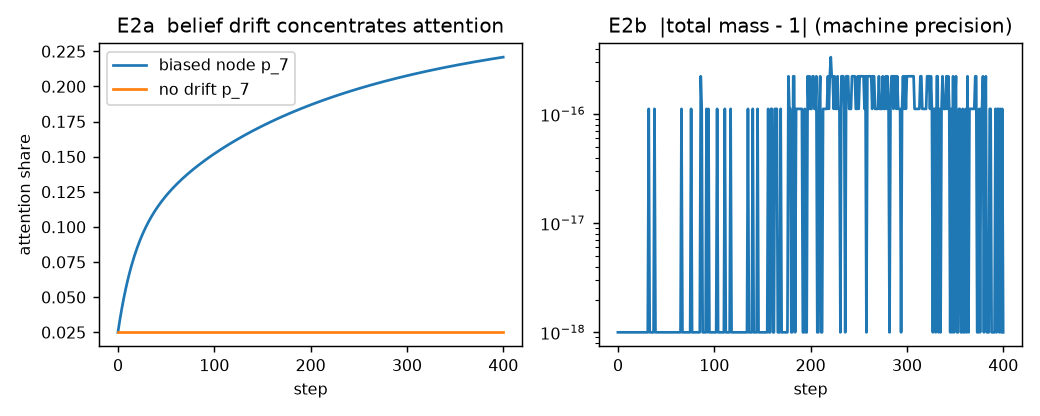
\includegraphics[width=0.92\textwidth]{_verify_out/E2_transport_drift.png}
\caption{Transport and belief drift (Eqs.~\eqref{eq:continuity}--\eqref{eq:flux},~\eqref{eq:master}). A belief field concentrates attention on a subset of topic nodes while total mass is conserved to machine precision (the conservation residual stays at the floating-point floor). This checks that the row-sum-zero generator of Eq.~\eqref{eq:master} preserves $\mathbf{1}^\top p$ under nontrivial drift, on the static graph that satisfies condition (C) of \S\ref{sec:transport}; exact conservation is claimed only on the static graph satisfying (C), the churning-node regime requiring a mass-conserving reassignment operator. Internal-consistency check of the paper's own equations on synthetic data.}
\label{fig:transport}
\end{figure}

\begin{figure}[t]
\centering
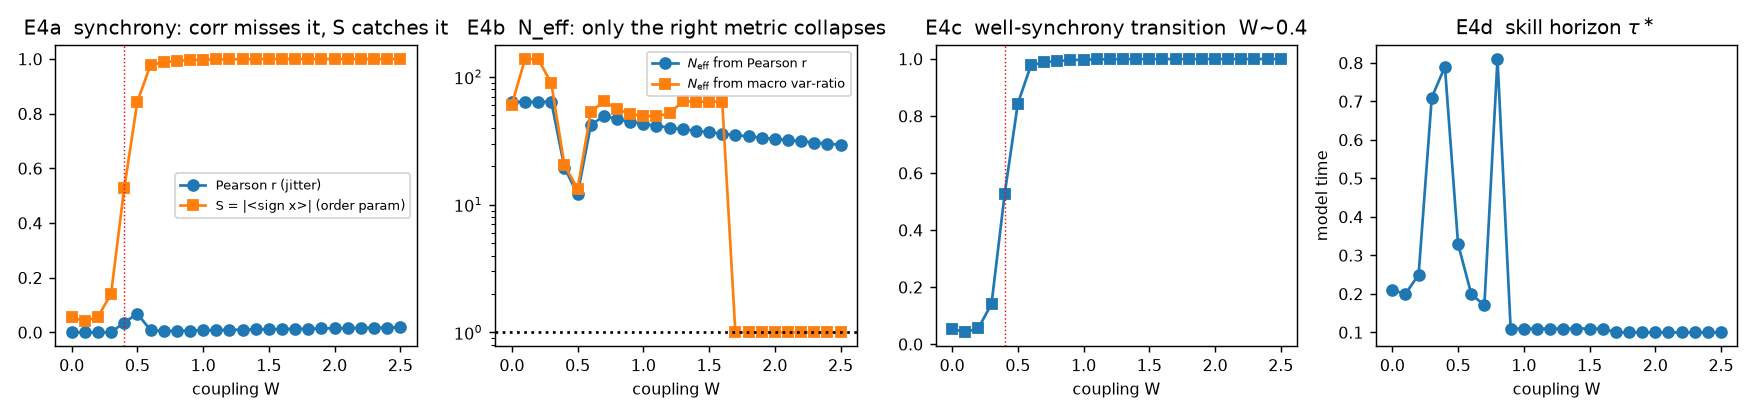
\includegraphics[width=0.92\textwidth]{_verify_out/E4_criticality.png}
\caption{Criticality across a coupling sweep (\S\ref{sec:criticality}). The numerical check uses a non-oscillatory mean-field surrogate (a coupled double-well system with no phase variable), whose synchrony observable is therefore the mean pairwise state correlation $\bar r$, not the Kuramoto phase coherence $r$ of \S\ref{sec:blocks}. As coupling rises, $\bar r$ increases and the $N_{\mathrm{eff}}$ of Eq.~\eqref{eq:kish} (fed $\bar r$ directly in place of $\varrho$) collapses toward $1$, and the skill horizon shrinks as the boundary is approached. The first-moment-versus-second-moment apparatus and the failing-fluctuation-correlation contrast of \S\ref{sec:blocks} are stated for the oscillator case they are defined on, which this surrogate leaves to that case. Internal-consistency check of the paper's own equations on synthetic data.}
\label{fig:criticality}
\end{figure}

\begin{figure}[t]
\centering
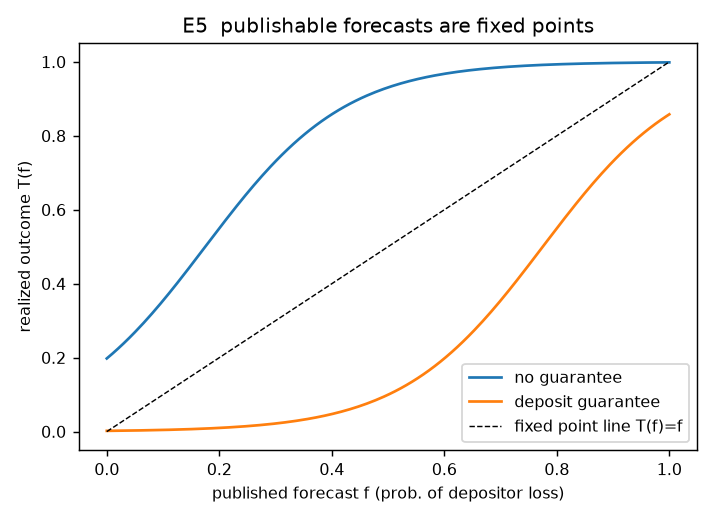
\includegraphics[width=0.92\textwidth]{_verify_out/E5_fixed_points.png}
\caption{The prediction--reaction map and its fixed points (\S\ref{sec:reflexivity}): the next-iterate map of the run probability plotted against itself, with fixed points at crossings of the 45-degree line. In the imitative regime the map has multiple fixed points (run and no-run); a credible all-deposit guarantee shifts the map below the diagonal so only the no-run crossing survives, illustrating the basin-selection control of \S\ref{sec:control}. Internal-consistency check of the paper's own equations on synthetic data.}
\label{fig:fixedpoints}
\end{figure}

Figure~\ref{fig:transport} checks conservation under belief drift; the mass error sits at machine precision, which is the structural-conservation claim of \S\ref{sec:engine} made visible. Figure~\ref{fig:criticality} demonstrates the $N_{\mathrm{eff}}$ metric collapsing toward $1$ as synchrony rises on the mean-field surrogate, the quantitative shape of the $\S\ref{sec:blocks}$ collapse (the first-moment-versus-second-moment contrast itself being reserved for the oscillator case, per the figure caption), and shows the skill horizon shrinking toward the transition. Figure~\ref{fig:fixedpoints} shows the reaction map's multiple fixed points and the guarantee killing the run, the quantitative echo of the SVB narrative. (Two further checks, a block law-of-large-numbers experiment and an early-warning trace, are available but omitted for space.) A fourth check (Fig.~\ref{fig:kuramoto}) tests the Kuramoto threshold of Eq.~\eqref{eq:kc} against finite-$N$ simulation ($N=2000$): for a heavy-tailed Lorentzian frequency distribution the empirical onset of synchronization matches $K_c=2/(\pi g(0))$ to within $3.1\%$ ($K_c^{\mathrm{theory}}=1.0$ versus $0.97$ empirical), while for a Gaussian distribution it matches only to $27.7\%$ ($1.60$ versus $1.15$), the discrepancy attributable to finite-$N$ and slow convergence near $K_c$ rather than to a failure of the law; we report both cases rather than the flattering one alone. None of these touches social data; they verify that the equations do what the text says they do.

\begin{figure}[t]
\centering
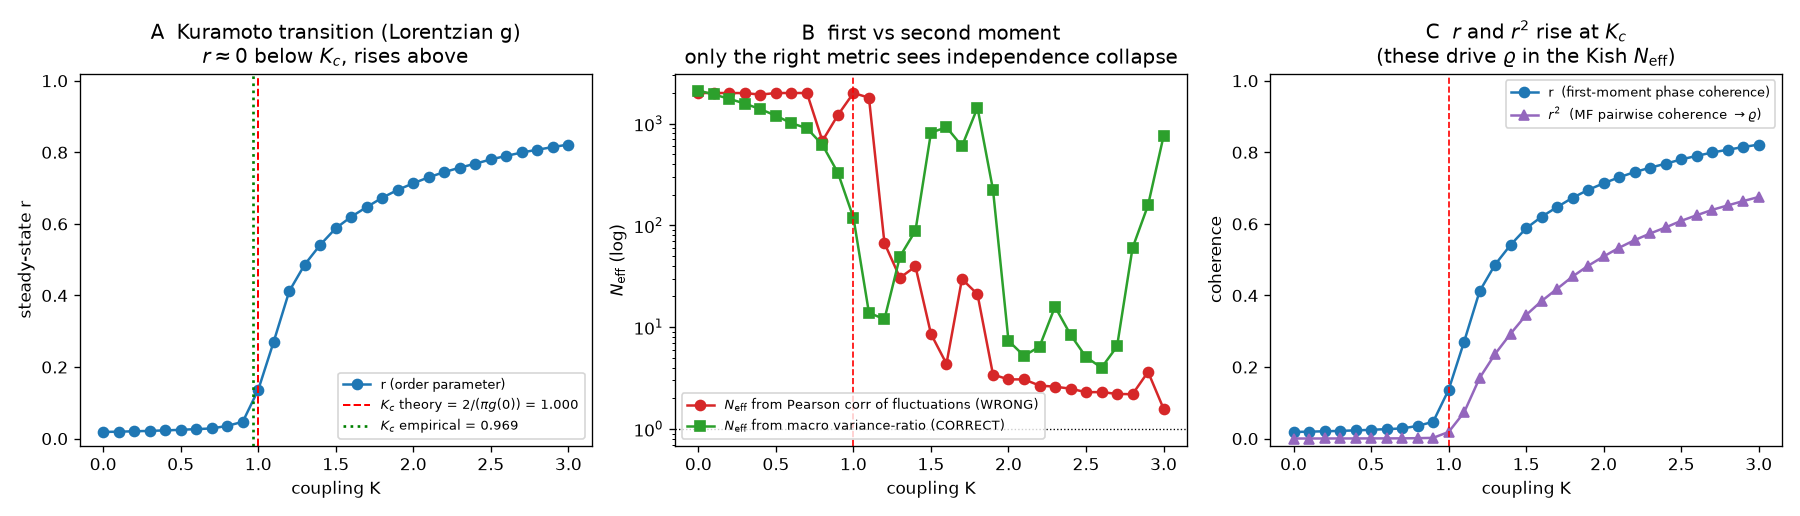
\includegraphics[width=0.92\textwidth]{validation/sims/kuramoto/kuramoto_kc.png}
\caption{The Kuramoto $K_c$ consistency check (Eq.~\eqref{eq:kc}, \S\ref{sec:blocks}): empirical onset of synchronization in a finite-$N$ simulation ($N=2000$) against the theoretical $K_c=2/(\pi g(0))$. The Lorentzian frequency distribution matches to $3.1\%$ and the Gaussian to $27.7\%$, the latter gap attributable to finite-$N$ and slow convergence near $K_c$. This is an internal-consistency check of the reused Strogatz result \cite{strogatz2000} on a controlled synthetic system.}
\label{fig:kuramoto}
\end{figure}

\section{Limits and the observability trilemma}
\label{sec:limits}

We state the limits as plainly as the claims.

\paragraph{Resolution limits.} In the smooth regime the system forecasts block-level aggregates over re-anchored horizons. It does not and cannot forecast individuals, and its equilibrium forecasts have resolution bounded by the equilibrium set whenever fixed points are non-unique.

\paragraph{The trilemma.} The two residual failure modes admit, between them, only one complete repair. Criticality can be managed by control but not predicted through. Misspecification can be detected and corrected after the fact but not anticipated. The single architecture that eliminates both, leaving no unpredictable branches and no out-of-distribution agents, is total observability of all components: the Galaxia limit. Prediction, agent independence, and bounded observation form a trilemma, and perfecting the first requires surrendering one of the other two. We name what the surrender of independence actually is, rather than admiring its symmetry: total observability is panopticon surveillance, and the abolition of agent independence is the end of the proposition that any individual can hold a belief the collective does not (it does not merely observe every person, it dissolves the boundary that makes a person a person). Asimov drew this limit too: in ``All the Troubles of the World'' (1958) Multivac predicts crimes before they happen by ingesting everyone's data, the total-observability-plus-prediction architecture in full, and the machine, made responsible for everything and able to validate nothing about its own purpose, wishes only to die, the terminal form of loading every burden and every judgment onto one locus accountable to nothing above it, which is the controller-cannot-validate-its-own-objective failure of \S\ref{sec:governance}, and specifically its condition (c) (the seer fused with the hand, fused further with the judge), taken to its terminus. We therefore do not push against this frontier; we reject it, and treat bounded predictability as the design goal and the unpredictable residue as the thing that protects pluralism. The governance content that makes this a structural stance rather than a lament is \S\ref{sec:governance}; we adopt Asimov's ambivalence here structurally, not only rhetorically. Asimov in fact stages the deliberate dismantling of the total-control optimum twice. In \emph{The End of Eternity} (1955) the organization ``Eternity'' edits history to remove every danger, and the cost of that relentless risk-minimization is stagnation: a humanity kept perfectly safe never takes the risks that interstellar travel requires, so when it finally ventures out the good worlds are already held by others and it declines. The resolution is to abolish Eternity on purpose, releasing an unguided, risk-taking humanity that expands first and founds the Galactic Empire.\footnote{The same future history then leads, through the Empire's decline, into the Foundation saga \cite{asimov1951}, so the paper's canonical spine spans Asimov's loosely unified corpus rather than \emph{Foundation} alone. The second staging is Galaxia's ambivalence in \emph{Foundation's Edge} (1982), where the total-integration optimum is reached but deliberately left contingent on a human chooser outside it.} The lesson we borrow is exact: total risk-minimizing control purchases safety at the price of the independence, risk, and growth a civilization needs to survive, which is why the control apparatus is dismantled rather than perfected, and which is the narrative form of our own rejection of total observability.

\paragraph{Scope of the position-paper hedge.} Calling this a position paper licenses the absence of \emph{results}; it does not license the absence of pre-committed, numeric falsification criteria, which we supply below regardless of implementation status. The hedge protects the lack of data, not the lack of testable claims. The internal numerical figures (\S\ref{sec:figures}) are consistency checks of the paper's own equations; their standing, like that of Proposition~\ref{prop:fixedpoint}, Asimov's fictional resolutions, and the SVB narrative, is illustrative of the framework's structure, with empirical confirmation reserved for the pre-registered tests above.

\paragraph{What would falsify the program.} The failure taxonomy of \S\ref{sec:failure} must not become an excuse generator: ``criticality'' and ``the Mule'' may be invoked only when declared \emph{ex ante}, never retrofitted to a miss. We therefore make the regime label (smooth / pre-critical / critical) and the out-of-distribution flag first-class, time-stamped outputs logged \emph{before} resolution to a third-party, append-only public registry (an OSF entry or a hash committed to a public ledger), since a label the authors timestamp privately is reconstructable after the fact; a forecast whose regime label is not externally timestamped prior to the resolution window is scored as a miss by default, and we commit that a forecast that misses while the engine declared ``smooth'' counts as a full refutation and may not be relabeled criticality or misspecification after the fact. With that seal in place, the operational tests are listed below. Each is written in the format that separates a genuine falsification test from a rhetorical one, and because that format is unfamiliar to many readers we name its parts plainly. A \emph{threshold} is the single number that decides pass or fail, fixed in advance. A \emph{null or base rate} is the chance-level performance the result must beat, so that a success cannot be claimed for an outcome that randomness or a naive guess would have produced anyway (this is the guard against the prosecutor's fallacy of \S\ref{sec:criticality}). A \emph{fixed sample frame} is the exact body of data the test runs on, named ahead of time so the result cannot be fished from a conveniently chosen subset. A \emph{horizon} is the time window over which the test is scored. A \emph{pre-registration commitment} means the entire specification, thresholds included, is time-stamped to a public registry \emph{before} the outcome is known. Stating each test this way is what removes the authors' freedom to move the goalposts after seeing the data. Several of these tests have now had a first pre-registered, powered run on retrospective data, reported inline in the items below and collected in \S\ref{sec:secondwave}; the rest remain commitments. We flag at the outset that the runs completed so far have mostly returned \emph{honest negatives or narrow positives}, which is itself the most important empirical news in this paper, and we mark each item's status explicitly rather than leaving the list as untested bets.
\begin{enumerate}[label=(\roman*),itemsep=2pt]
\item \emph{Conservation / zero-sum.} Across the $N$ most-trafficked platforms over rolling 90-day windows from a pre-registered start date, aggregate human attention-minutes vary by less than a committed $X$ percent, \emph{net of the demographically-predicted source growth $\int\dot A\,dt$ over the window}, while composition churns by more than a committed $Y$ percent. Conservation is refuted if cross-platform attention-minutes expand by more than $X$ percent, net of that predicted source growth, during at least one documented mania. Separately, the slow source itself is bounded: the trailing 12-month growth in aggregate attention-minutes must stay below a committed $Z$ percent per year, an endowment that grows faster than $Z$ refuting the sub-generational-budget premise of \S\ref{sec:attention} independently of any single mania. The same total must hold (within $X$) even at criticality; ballooning totals during a panic refute the law where it most needs to bind. \emph{First run (\S\ref{sec:secondwave}): contradicted at the basket scale.} A nine-subreddit finance and meme-stock basket over the January-2021 squeeze saw its total submission activity expand roughly fourteen-fold while composition churned, far past any reasonable $X$. The honest qualification is that a related-subreddit basket is a porous boundary, so a local balloon is consistent with global conservation plus import from outside the basket; the run refutes conservation \emph{at the basket scale} and leaves the whole-platform claim of this item untested, matching rather than rescuing the earlier single-subreddit pilot.
\item \emph{Block independence.} Community blocks recovered by a named algorithm at a fixed resolution exhibit cross-block fluctuation correlation below a committed $\varrho_0$ in calm regimes across a named interaction-graph corpus. Block independence is refuted if $\varrho$ exceeds $\varrho_0$ in the median calm window.
\item[(ii$'$)] \emph{Dynamic $N_{\mathrm{eff}}$ collapse (the load-bearing unconfirmed gear).} The criticality account of \S\ref{sec:blocks} and \S\ref{sec:control} rests not on blocks being distinct in calm (test (ii)) but on the effective number of \emph{independent} blocks collapsing across an onset, the recovered law of large numbers evaporating exactly when stakes peak. We name this separately because it is the single mechanism the whole criticality story turns on and the one the blind pilot of \S\ref{sec:obsupgrades} left at $n=1$. Operationally: on a frozen roster of $M'$ labelled endogenous cascades each carrying a usable pre-onset interaction graph, the Kish $N_{\mathrm{eff}}$ (Eq.~\eqref{eq:kish}) must fall by at least a committed fraction $f$ from a pre-onset baseline window into the onset window, scored against a null of matched calm-window pairs drawn from the same series; if the median collapse fails to reach $f$, the synchronization-at-criticality mechanism is refuted as written. This test has now had a powered, pre-registered, two-substrate run (\S\ref{sec:neffcollapse}, $f=0.30$ frozen before harvest): the collapse is real, event-specific, and community-specific on the substrate that has communities (r/wallstreetbets, $9$ of $10$ cascades beat the shuffle null), but the per-substrate median collapse (Wikipedia $0.19$, Reddit $0.22$) falls below the committed $f$, so by this sealed rule the mechanism is \emph{measured and directionally supported but not yet confirmed}. That clean-pass attempt has since been run (\S\ref{sec:neffcollapse}): with the threshold re-derived principledly ($f=0.298$, the $95$th percentile of the collapse that genuinely-quiet windows themselves produce, an engine cross-check putting the physically attainable collapse near $0.7$ to $0.8$) and frozen before a \emph{fresh} roster disjoint from the tuning set, the median collapse was $0.00$ and the sealed rule was \emph{not} met. The collapse is therefore confirmed real but \emph{endogenous-specific}: it cleared $f$ on the endogenous balance-sheet failures in the fresh roster (Lehman, the FTX founder's collapse) and vanished on its exogenous-shock majority, whose onsets dilute the frozen blocks with newcomers. The gear turns, but only in the special regime, and a roster's measured collapse tracks its endogenous fraction.
\item \emph{Early warning.} On a frozen, pre-registered roster of $M$ candidate fold-type transitions selected \emph{before} outcomes are known, the Scheffer early-warning battery with the Boettiger null \cite{scheffer2009,boettiger2012} achieves an area-under-the-ROC-curve (AUC) above a committed value against a stated base rate, with the N-/R-tipping exclusion declared in advance. This test is explicitly weakened by the N-/R-tipping blind spot of \S\ref{sec:criticality}, and its honest form is the sharper bet (iii$'$) below. \emph{First run (\S\ref{sec:secondwave}): partial positive.} A powered run of the \emph{semantic} variant of this battery across ten r/wallstreetbets cascades beats a guard-banded calm null ($p=0.02$, five of five endogenous events above their own calm window) but does \emph{not} discriminate endogenous from exogenous builds (AUC $0.60$); it detects that a belief build is underway, not which kind, which tempers the clean-looking $n=2$ pilot of \S\ref{sec:obsupgrades}.
\item[(iii$'$)] \emph{Bifurcation-mix conjecture.} The program's predictive value rests on the conjecture that decision-relevant social crises are \emph{predominantly} B-tipping rather than N- or R-tipping. Operationally: on the frozen roster of $M$ resolved crises of test~(iii), each is post-hoc adjudicated as B-, N-, or R-tipping by a pre-declared classification rule applied by raters blind to the early-warning scores, and the conjecture is refuted if the B-tipping fraction falls below a committed $\pi_B$. This is the test most likely to fail, and we name it as such. \emph{First run (\S\ref{sec:secondwave}): refuted.} On a 24-cascade labelled roster the substantive B-tipping fraction is $0.33$, below $\pi_B=0.60$, with most cascades adjudicated as sudden R-tipping shocks. A purely structural proxy gave $0.75$ but is an artifact of single-venue author-pool saturation; we report the refuting substantive number, not the passing artifact. The bet we named as most likely to fail did fail, on this roster.
\item \emph{Smooth-regime skill.} Against a pre-registered question set of size $m$, the engine must achieve a Brier score at least a committed $\delta$ below the relevant superforecaster or market-implied baseline, or the smooth-regime claim is refuted.
\item \emph{Fixed-point reliability.} Credibly published fixed-point forecasts must hold more often than a naive base rate on a pre-registered set of policy announcements, with the publishable/non-publishable classification declared ex ante; if they fail more often than the base rate, the reflexivity repair is refuted.
\item \emph{Lucas invariance.} The calibrated coefficients ($\theta_S$, $v_k$, $D_k$, $W$, $\Phi$) must remain stable across a pre-declared regime break beyond what online assimilation can absorb within its lag; large structural drift refutes the claim that the engine is more than a reduced-form fit.
\item \emph{Regime occupancy (the Soros bet).} On a named market-or-platform series over a pre-registered span, the fraction of windows classified imitative by the regime monitor stays below the monotone fraction; if imitative windows dominate, the monotone-exception bet of \S\ref{sec:reflexivity} (and the disagreement with strong reflexivity) is refuted in favor of generic reflexivity. The classification is by realized variance share as well as window count, so the test does not let the rare imitative regime hide behind its small calendar footprint.
\end{enumerate}
The numeric thresholds ($X$, $Y$, $Z$, $\varrho_0$, $M'$, $f$, $M$, $\pi_B$, AUC, $m$, $\delta$) are to be fixed and time-stamped at pre-registration; until then the honest statement is that none of these is yet operationalized against data. These criteria bear on whether the program is \emph{correct}, not on whether it is \emph{safe to deploy}; a confirmed program raises the governance stakes of \S\ref{sec:governance} rather than lowering them.

\section{First empirical contact}
\label{sec:empirical}

We report preliminary first-contact results on real data; these are pilot runs of the pre-registered tests of \S\ref{sec:limits}, illustrative and suggestive in direction at small $n$. They are numerical in the same sense as the synthetic illustrations of \S\ref{sec:figures}, and are a higher class of evidence (\S\ref{sec:figures}) for the single reason that they run on real social data rather than synthetic data, not because they are a different kind of activity. They instantiate the test \emph{designs} of three of those tests, executed on attention series harvested from the Arctic Shift API, a reachable Reddit-archive host, at weekly and monthly resolution. We state the limits before the results, because they govern everything below.

\emph{First, the status.} Every run below is a retrospective backtest on events whose outcomes were already known when the analysis was designed (GameStop 2021, the 2022 energy and inflation shocks, the 2025 tariff shock), not a forward, pre-registered forecast of the kind \S\ref{sec:limits} commits to. None was time-stamped to the public registry before its outcome, and the pre-registration thresholds of the companion artifact are marked \emph{proposed} and not yet lodged to an external registry, so at submission no test is frozen and these pilots set thresholds with data in view. None of these runs can therefore discharge any of the pre-registered falsification tests, and none carries pre-registered evidentiary weight. They are reported to demonstrate the pipeline and to locate the program's empirical bet, not to score the falsification tests, which remain open. These pilots also exercise three isolated diagnostics (an early-warning detector, an overdetermination check, and a major-player ramp detector); they do not instantiate the assimilation engine of \S\ref{sec:engine} (no forward model, no EnKF, no coupling matrix $W$, no reanalysis corpus), which still awaits that corpus.

\emph{Second, the observable.} The observable is mention-density: how many posts per hour mention a given topic, a proxy for how much a community is talking about it. (It is computed as an inverse-inter-arrival density over the first hundred posts of each bucket from the Arctic Shift \texttt{/api/posts/search} endpoint; the hundred-record cap biases very high-volume weeks toward shorter spans, i.e.\ toward exactly the onset weeks, a bias we flag and return to. The aggregate-count endpoint was unusable because it returns all-zero counts for r/wallstreetbets and HTTP~422 throttling, so one density method is used for every event. The full rosters, formulas, and per-event result files are in the companion \texttt{validation/backtests/} tree.) The observable is one step removed from every quantity the theory is actually about: not order flow, not price, not short interest, and not sentiment or belief. More precisely, mention-density is essentially the scalar magnitude of the attention flux, the rate at which attention flows onto a topic, a scalar projection that discards the \emph{direction} of the belief-drift field $b$ and the valence, so the pilots measure a coarse scalar shadow of the vector transport theory rather than the vector theory itself: the continuous-time transport and mean-field-game equations are the idealized framework, and these pilots are a deliberately coarse first contact with it. That coarseness bears \emph{asymmetrically} on the three pilots. Critical slowing-down is a second-moment, autocorrelation-structure signature that is especially fragile under a coarse, capped, rate-only proxy, whereas the first-moment features the other two pilots read (gross simultaneity, ramp duration) are far more robust to it, so part of any null in the first pilot may be the instrument rather than the world.

\emph{Third, the rosters and labels.} The rosters are small, several events share a subreddit and so are not independent, the mention-rate series for GameStop is measured on the very forum the operator posted to and the platform's ranking amplified (so it is a contaminated crowd-attention proxy there), and the onset and endogenous-versus-exogenous labels are judgment calls. These are therefore illustrative first-contact runs on proxy data, suggestive in direction at small $n$, and we will repeat that framing where it bears weight rather than rely on this paragraph to carry it. We also note that the harvested attention history and the per-individual buildup series this section produces are, at small scale, the controller-precursor data that \S\ref{sec:governance} governs; we hold and disclose them under the same logged, auditable, monitor-versus-hand standard the paper demands of others.

The value of the exercise is not confirmation. It is that the data, even at this resolution, discriminate sharply between the three mechanisms the framework names, and they do not discriminate in the program's favor uniformly. One of the three came back negative, and it is the one the paper's own bifurcation-mix conjecture (test~(iii$'$)) predicted would fail.

\paragraph{Pilot 1: the impersonal early-warning signal does not generalize.} The first run is the honest negative. We assembled a labeled battery of ten events (six endogenous cascades, four exogenous shocks) and ran the literature-standard early-warning detector with a strict pre-onset information cutoff and a base-rate null (the prosecutor's-fallacy guard of \cite{boettiger2012} over the Scheffer battery \cite{scheffer2009}). The detector is the detrended critical-slowing-down detector: on the six-week window ending the week before onset, it takes a $\log$ transform, subtracts a moving-average trend, and scores the sum of two Kendall-$\tau$ trend tests (a Kendall-$\tau$ measures whether a series is trending up, here whether the rolling variance and the rolling lag-1 autocorrelation rise into onset), against a sliding non-onset null. Every AUC below is the win-fraction of the onset window against that series-specific null, so AUCs are not directly comparable across series with very different null lengths.\footnote{The AUC (area under the ROC curve) is a detector-accuracy score running from $0.5$ for coin-flip guessing to $1.0$ for a perfect detector; below $0.5$ is worse than chance. The percentile reported alongside it is the strict fraction of null windows the onset window beats, and the two differ because the AUC splits ties.} We are explicit that the detector family itself was selected after inspecting the data and was \emph{not} pre-registered, so every AUC in this pilot inherits a detector-choice degree of freedom. The six-week detector window is one such unregistered choice, and Table~\ref{tab:window} makes its consequence fully transparent.

The cleanest endogenous cascades show the signal as predicted: GameStop scores an AUC of $0.915$, and separately its approach window sits at the $83$rd percentile of the non-onset null (a top-$17\%$ tail, $z=1.38$, not individually significant for a single series), while Superstonk scores AUC $0.78$, the detrended rolling variance rising monotonically into onset. We keep AUC and percentile distinct because they are different statistics: an AUC of $0.915$ corresponds by itself to roughly an $8.5\%$ tail, and the $17\%$ figure comes from the percentile $0.83$, not from the AUC. But the aggregate dissociation washes out. The six endogenous AUCs are $0.915$, $0.78$, $0.53$, $0.50$, $0.21$, $0.06$, a bimodal split of two clean positives against four chance-or-below cases, not a uniform null; their mean is $0.500$ against an exogenous mean of $0.487$, a separation of $+0.012$. With six endogenous and four exogenous events the rank test is severely underpowered: a Mann-Whitney $U$ test (a standard test for whether two groups differ) at this sample size cannot attain $p<0.05$ even under complete separation, so the reported $p=0.91$ (asymptotic; the exact permutation null over the $\binom{10}{4}=210$ rank assignments is the correct object and likewise non-significant) records a \emph{failure to detect} a dissociation, not evidence of its absence. The between-group rank effect size is itself $0.479$, slightly below $0.5$, i.e.\ a random endogenous event is marginally \emph{less} likely to outscore a random exogenous one, which straddles chance and reinforces the honest-negative reading rather than weakening it. The non-independence makes this weaker still: three of the six endogenous cases (GameStop, Superstonk, and the WSB meme-basket) are the \emph{same} January-2021 WSB excursion, which the paper's own correlated-agents argument (O3, \S\ref{sec:objections}) forbids counting as independent, so the effective independent endogenous count is about four, and the test is even more underpowered than $n=6$ implies.

One detail is worth stating, but as a forking-paths hazard rather than a virtuous self-correction. An earlier naive rising-variance detector had scored a single case, the 2022 European energy crisis, at an AUC of $1.0$ (a maximally false alarm, $z\approx 22$, fooled by the post-onset spike polluting its null), and the detrended Kendall-$\tau$ detector drove it to $0.21$. That $0.79$-of-AUC swing on one case from one detector swap is the magnitude of the detector-choice degree of freedom, not merely a bug fix, and the same un-pre-registered choice produced every other AUC here including GameStop's $0.915$. It also costs the framework a predicted hit, not just an inflated one: per the roster the European energy crisis is a \emph{labeled endogenous} case, a case the framework expected to be a positive, so its detrended $0.21$ is a \emph{missed predicted positive}, and the more honest detector removes one of the framework's own expected hits at the same time as it removes an inflated alarm. We state both halves rather than spin the miss as a self-correction.

The honest reading is not that the framework failed but that one of its mechanisms did not generalize across a heterogeneous roster, which is \emph{consistent with} (not a confirmation of) the bifurcation-mix conjecture (test~(iii$'$) of \S\ref{sec:limits}): if most social transitions are not clean fold-type B-tipping, the impersonal critical-slowing-down tremor should fire on the cleanest fold-like cascades and wash out across a mixed roster, and that is what it did. We are careful that a null is weaker than a confirmation. The wash-out is equally consistent with the rival explanations that the rate-only proxy is too coarse to carry a second-moment critical-slowing-down signature, or that ten events have no power to separate the groups; we have not excluded these, so test~(iii$'$) is not made unlosable, and the conjecture's own pre-registered adjudication (B- versus N-/R-tipping by blind raters) remains unrun. The framework named the location of a possible weakness and the weakness appeared there, but the naming is registered \emph{before} this section and the directional prediction was not externally time-stamped against this roster, so we read it as consistency, not as a costless prediction.

The detector window is itself an un-pre-registered choice of the same kind as the detector family, and we expose it directly rather than report only the window that flatters the headline. Table~\ref{tab:window} sweeps the GameStop AUC across the four candidate windows. The headline six-week window gives $0.915$; widening to ten weeks drives it to $0.379$, below chance, and the full spread from $0.915$ to $0.379$ is the magnitude of this single researcher degree of freedom. The headline is therefore not a robust property of the series but a property of the series read through one unregistered window.

\begin{table}[h]
\centering
\begin{tabular}{@{}cc@{}}
\toprule
\textbf{Detector window (weeks)} & \textbf{GameStop AUC} \\
\midrule
6 (headline) & 0.915 \\
8 & 0.771 \\
10 & 0.379 \\
12 & 0.435 \\
\bottomrule
\end{tabular}
\caption{GameStop early-warning AUC across detector-window choices (window sweep from the aggregate result file \texttt{validation/backtests/early\_warning\_battery/results/\_aggregate.json}). The headline $0.915$ uses the six-week window; the result is sensitive to this unregistered choice, falling to below-chance ($0.379$) at ten weeks. The spread across windows, from $0.915$ down to $0.379$, is the magnitude of this single researcher degree of freedom, reported here so the forking path is fully transparent rather than buried in the headline number.}
\label{tab:window}
\end{table}

\paragraph{Pilot 2: structural overdetermination is supported.} The thesis first, then the ladder that supports it: the episode is a Seldon crisis at the aggregate and a Mule at the branch, and the two verdicts live at different resolutions. The second run uses the January 2021 GameStop squeeze as an observational case study (a single real-world episode read in place of a controlled experiment) of the paper's signature distinction, the Seldon crisis (structurally determined aggregate) against the Mule (the indispensable individual operator). For readers who missed the 2021 news: a short squeeze occurs when many traders have sold a stock short (borrowed and sold it, betting the price falls) and a rising price forces them to buy back at once, driving it higher still; GameStop's short interest exceeded one hundred percent of its float (more shares had been sold short than existed to buy back), which guarantees such a scramble. This is not a true counterfactual (we cannot observe the no-operator world to compare against), so it tests two structural signatures instead. First, susceptibility was building independently of any operator: r/wallstreetbets activity rose roughly sixfold across 2019--2020 (mean about $4.3$ posts per hour in 2019 to about $25.9$ in December 2020, from the longer 2019--2021 activity harvest, distinct from the six-week onset series above), the rise complete \emph{before} the GameStop spike. Second, the basket co-moved: all six tracked tickers (GME, AMC, BB, NOK, BBBY, KOSS) reached their mention-density peak in the same week, 2021-01-31, with GameStop's own ramp leading the others' onset by about six to seven weeks before the basket squeezed together. We flag that this co-peak is not six independent ignitions: once GameStop moved, cross-shorted-basket covering, retail attention spillover into adjacent names, and correlated dealer hedging mechanically couple the tickers, so the simultaneity is partly endogenous to the lead event and overstates the independence of the sparks. The six-ticker basket is also itself selected on the outcome (these names are remembered precisely because they co-peaked), so the simultaneous-peak finding cannot be read as overdetermination without a candidate basket fixed before the peaks were known. Figure~\ref{fig:counterfactual} shows the three structural traces this pilot reads: the multi-year r/wallstreetbets activity build, the six-ticker simultaneous mention-density peak, and the DFV posting timeline.

\begin{figure}[t]
\centering
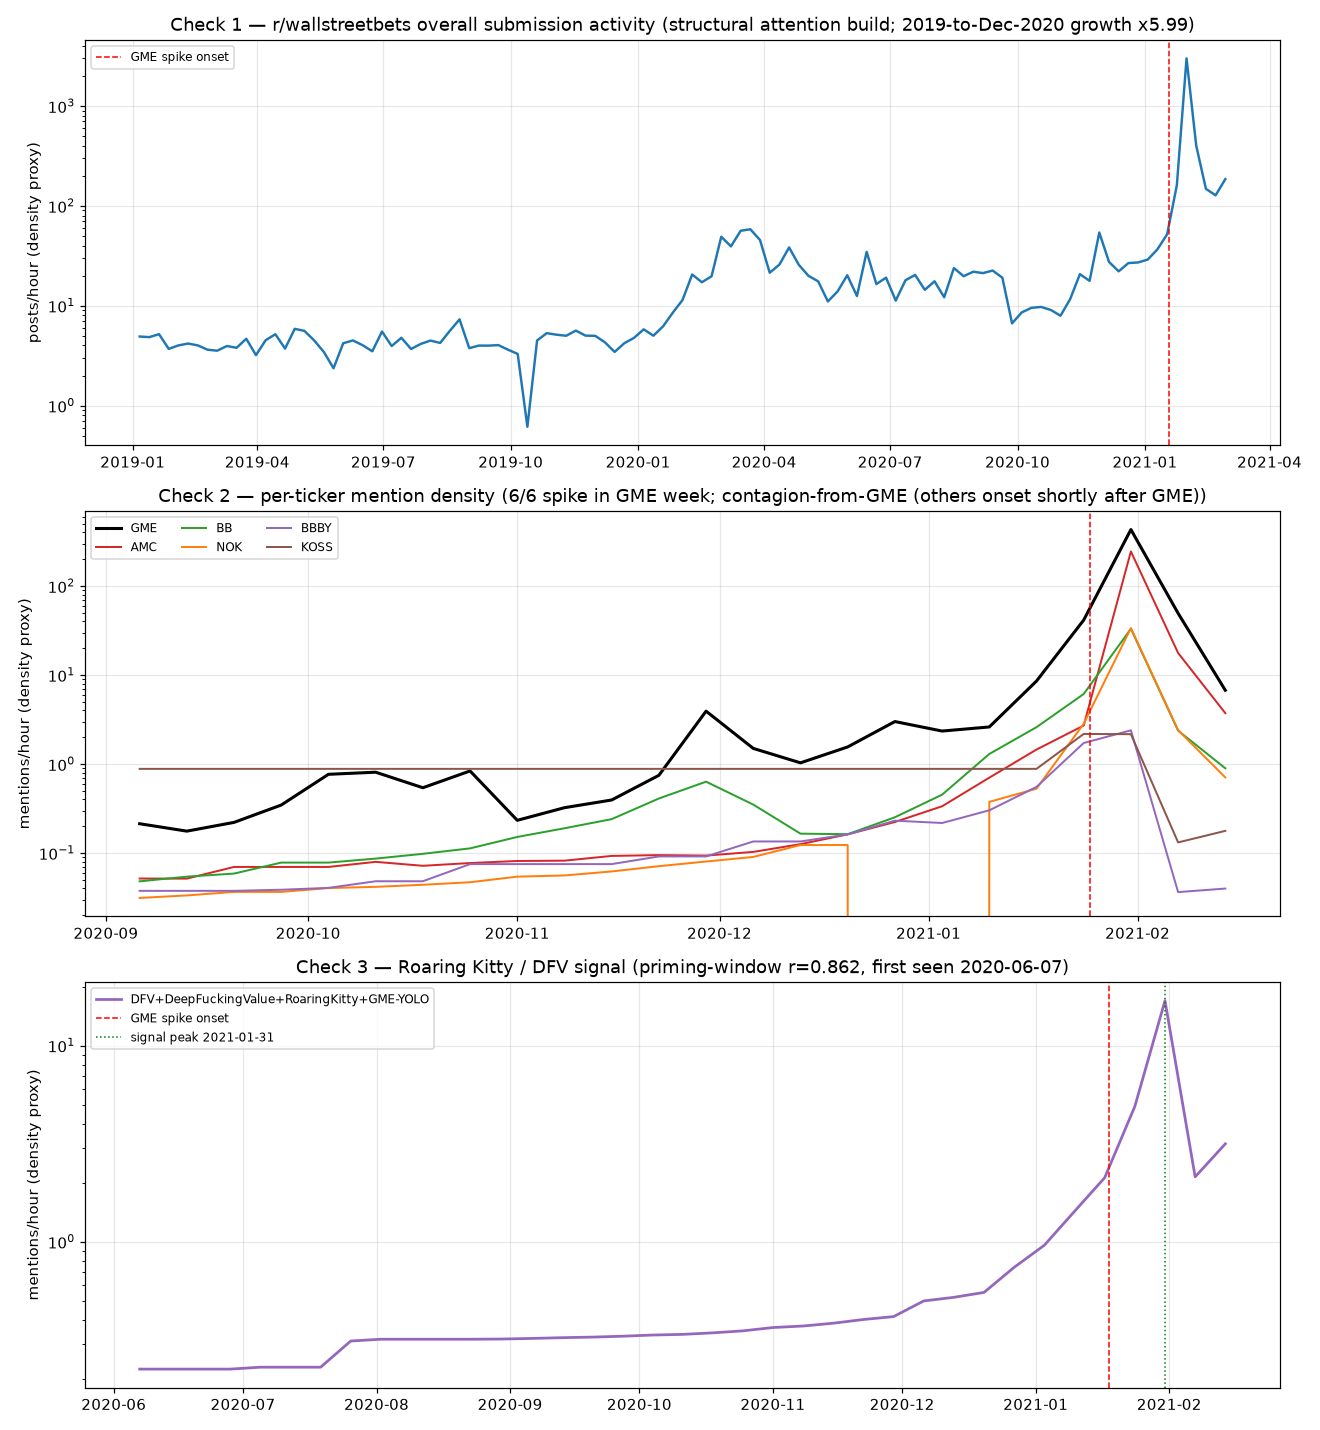
\includegraphics[width=0.95\textwidth]{validation/backtests/gamestop_counterfactual/figure_counterfactual.png}
\caption{Pilot 2, structural traces of the January 2021 GameStop episode: the multi-year build of r/wallstreetbets activity (susceptibility rising before the spike), the six tracked tickers reaching their mention-density peak in the same week, and the DFV / Roaring Kitty posting timeline. Preliminary first-contact result on proxy (mention-density) data harvested from a Reddit archive at small $n$; the six-ticker basket is selected on the outcome and the co-peak is partly endogenous to the lead event, so this is illustrative of the overdetermination-plus-operator reading, with the directions suggestive.}
\label{fig:counterfactual}
\end{figure}

The verdict resolves at three resolutions, and the resolution is the point. COARSE (would a squeeze happen at all) is \emph{consistent with} overdetermination (it had so many independent triggers primed that a squeeze would plausibly have happened by one route or another even without any single operator), a candidate Seldon crisis in the structural-inevitability sense, that \emph{some} squeeze was overdetermined even though its branch was not: the powder keg was full and multiple tickers primed together, though a single operator priming the whole basket is not excluded at this resolution. MEDIUM (which flagship, what magnitude, in which week) is operator-shaped: the operator preheated GameStop specifically and selected the flagship and the timing, and GameStop's structural fragility, the short interest above one hundred percent of float (a GME-specific fact, not a basket-wide one; AMC, NOK, and BB carried no comparable ratio), is itself a flagship-selecting fact that belongs here rather than to the COARSE bucket. FINE (this exact path) splits by causal category: the gamma-squeeze dealer-hedging loop is an endogenous mechanical amplifier, the brokerage buy-button halt (the day retail brokers blocked new purchases) was an \emph{exogenous} clearinghouse-collateral event forced by a roughly tenfold spike in the broker's NSCC clearing-deposit requirement, institutional plumbing that no operator chose and that is distinct from the gamma loop, and only the operator's flagship-and-timing choice is operator-contingent. This is the framework's signature claim made concrete: the aggregate is structurally determined while the individual operator selects the branch. It is the butterfly-at-criticality reconciliation of \S\ref{sec:control} (the operator exercises leverage precisely where the statistics fall silent) and the individual-versus-aggregate split of \S\ref{sec:mule} (a Seldon crisis at the aggregate, a Mule only at the fine branch), observed rather than merely argued, and it is the small-scale, single-operator instance of the loss-of-plurality mechanism of \S\ref{sec:mythosfable}: an operator selecting one branch for a primed basket is what a frontier model selecting one branch for a homogenized population looks like with $N_{\mathrm{eff}}$ near one.

We are careful not to overclaim the operator's agency. The market record is consistent with the Roaring Kitty / DFV posts as a \emph{focal coordination device}, making an existing latent fixed point common knowledge (the reflexivity common-knowledge mechanism of \S\ref{sec:reflexivity}, the Seldon-trial structure), rather than a controller who steered the crowd; ``operator'' is the stronger of two live hypotheses that weekly resolution cannot separate, and the common-knowledge reading also resolves a tension, since single-agent control in the paper's formalism requires non-negligible measure, which a retail poster with no capital to deploy at scale lacks. We hold the honesty line: this is one selected episode at coarse weekly resolution, suggestive of overdetermination, not a proof that the operator was dispensable. And it carries a governance inversion we name rather than bury: overdetermination cuts against \emph{targeted} suppression (no single operator is decisive) but thereby cuts \emph{toward} block-scale suppression (a party who cannot stop the cascade by removing one person is pushed to act on the whole susceptible community), which is exactly the collective punishment the moral-concern rule and conditions (a)--(d) of \S\ref{sec:governance} forbid. The same finding that is evidence \emph{for} the structural account is a hazard pointing at mass coercion.

\paragraph{Pilot 3: the operator-signal detector discriminates on illustrative cases.} Since the impersonal tremor did not generalize and the mechanism the framework actually rests on is operator skill at criticality (\S\ref{sec:control}), the third run tests the operator signal directly with a major-player-buildup detector. The discriminating quantity it reads is the \emph{duration} of the pre-onset operator ramp: the Roaring Kitty / DFV signal ramps for thirteen consecutive weeks into onset at about $+18\%$ per week, though it peaks in the \emph{same} week as the crowd, so the thirteen weeks is a ramp duration and not a lead time. The two AskEconomics shocks ramp for only two to three weeks. From this duration plus the ramp slope and level correlation, a sign-conventioned composite index (defined in the companion artifact; positive marks a sustained internal-operator buildup, negative a sudden external shock, zero the dividing line) places GameStop at $+3.54$ and the 2025 tariff shock and 2022 inflation surge at $-2.25$ and $-2.19$. We lead with the ramp-duration discriminator because the composite is a derived index of ramp \emph{strength}, not of the duration the prose names, and reporting it to two decimals on this sample would read as a precision the construction does not have. Figure~\ref{fig:majorplayer} contrasts the operator signal against the aggregate crowd series, GameStop against the two AskEconomics shocks. We separate two distinct claims this detector bundles together, because the cross-domain replication of \S\ref{sec:githubrep} pulls them apart: operator \emph{concentration} (that a single dominant driver exists at all) is the candidate domain-general invariant, while the gradual multi-week \emph{buildup} duration is the platform-specific signature that discriminated this Reddit case, and only the former is expected to travel.

\begin{figure}[t]
\centering
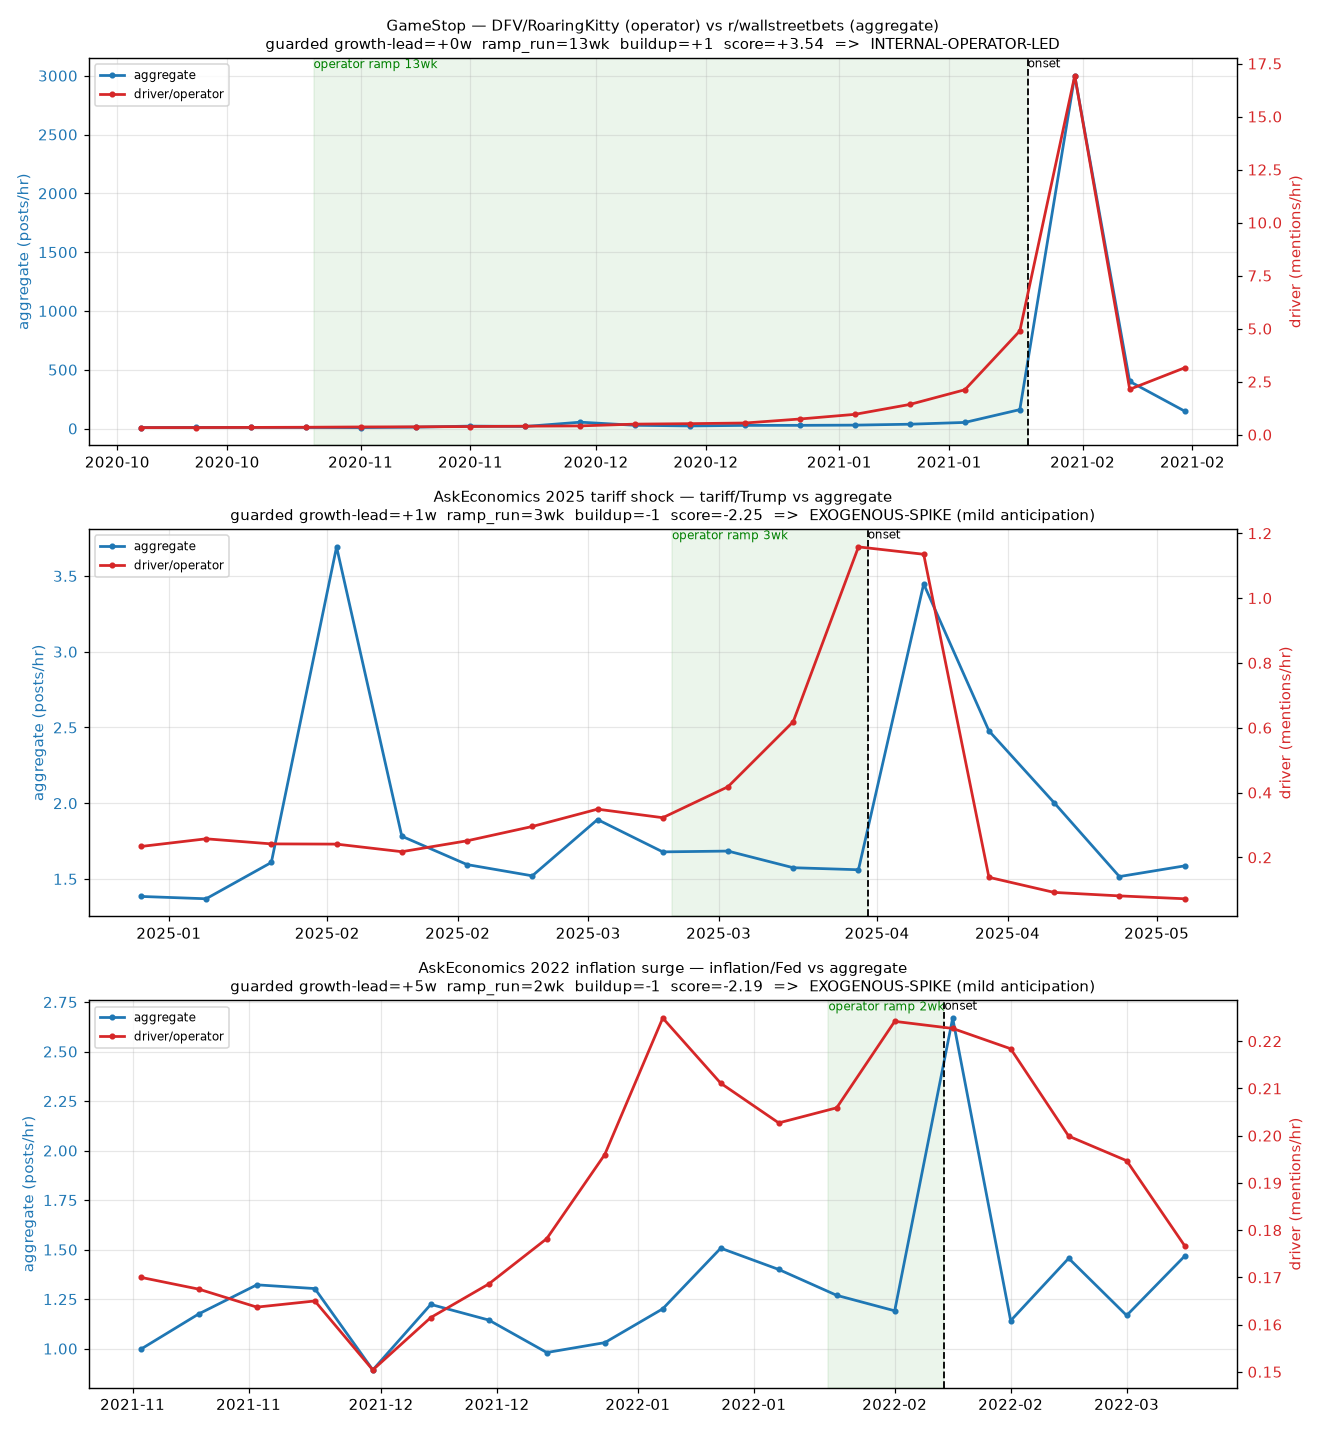
\includegraphics[width=0.95\textwidth]{validation/backtests/major_player_signal/figure_major_player.png}
\caption{Pilot 3, the operator-signal detector: the major-player buildup (DFV / Roaring Kitty) against the aggregate crowd series for GameStop, contrasted with the two AskEconomics shocks (2025 tariff, 2022 inflation). The operator signal ramps for thirteen consecutive weeks into onset; the exogenous shocks ramp for only two to three. Preliminary first-contact result on proxy (mention-density) data with thresholds set in view of the data, illustrative of the mechanism classifier (gradual internal buildup versus sudden external shock), with the pre-registered tests of \S\ref{sec:limits} still open.}
\label{fig:majorplayer}
\end{figure}

We are explicit and unflattering about the lead-lag. The driver's and the crowd's week-over-week changes cross-correlate with their peak at lag zero in weekly buckets, so any true Roaring Kitty-to-crowd lead is bounded by the one-week sampling interval and is not resolved; the true lead was days, below that floor, and the detector makes no use of it. What the detector therefore separates is a gradual internal-operator buildup from a sudden external shock. It is a mechanism classifier, not a several-weeks-ahead alarm, and we do not dress it up as the latter. We also cannot, with mention-density alone, separate an operator buildup from the gradual arrival of genuine fundamental catalysts over the same quarter (the Ryan Cohen stake, the new-console demand cycle, the pre-existing deep-value thesis), which generate the same monotone multi-week ramp; distinguishing them would require differencing the operator's idiosyncratic posting against the fundamental news flow, which we have not done, so the operator reading here is unidentified against slow good-news arrival.

The two ``exogenous'' contrasts are not clean exogenous impulses, and we relabel accordingly. We use \emph{exogenous} in the narrow forum-relative sense of ``not generated by an operator internal to the tracked community.'' A tariff announcement is itself a major-player strategic act in the \S\ref{sec:engine} taxonomy (telegraphed, partly anticipated, not an act of nature), and the 2022 inflation surge was a slow, widely-forecast macro process whose forum \emph{attention} spiked even though the fundamental did not. The detector separates internal-operator buildup from forum-exogenous attention spikes, not policy-exogenous from fundamentals-exogenous shocks. The sample is three events (one operator-led, two exogenous) in two mechanism classes, with the single tariff onset taken as 2025-04-07 throughout, and with thresholds set in view of the data. This explicitly violates the pre-registration discipline of \S\ref{sec:limits} (which forbids in-sample threshold-setting) and is reported as mechanism-illustration only: it earns no credit against any scored falsification test, a calibrated version falls under that pre-registration discipline (time-stamped thresholds, null, and roster before resolution), and the present in-sample figures carry zero confirmatory weight.

\emph{Governance status of this detector.} We flag its dual-use status explicitly, because this is the one place the manuscript demonstrates an offensive-adjacent primitive working on real data, and \S\ref{sec:governance} was written before it existed. A major-player-buildup signal is the offensive primitive of \S\ref{sec:governance} read in the defensive direction: the same ramp that warns a population an operator is building a position tells a hostile party whom to target, suppress, or co-opt before they move the crowd, which is the pre-crime structure (acting on a prediction of future influence rather than on a completed act). Its asymmetry therefore does \emph{not} run defensive-dominant, unlike the block-level regime monitor, so it falls outside the publish-in-full defensive bucket of \S\ref{sec:governance}: it is governed by the offensive-layer conditions (a)--(d) and the monitor-versus-hand separation, published only at the aggregate mechanism-classifier grain (gradual-internal-buildup versus sudden-external-shock) and \emph{never} as a named-individual identifier or a pre-onset alarm against a specific person. The sign test of \S\ref{sec:governance} scores interventions, not detections, so it cannot reach this capability; a detector of this kind is instead governed at the disclosure and access layer, defensive when its output is a population-facing warning that raises the population's own $N_{\mathrm{eff}}$ and offensive when its output is a private target list that lowers it. We hedge the demonstration: it was run retrospectively on a public, already-resolved episode and a self-identified public individual, we publish only the mechanism-classifier verdict and the aggregate ramp-duration statistic, and we withhold the per-individual scoring calibration a prospective targeting use would need, holding the harvested data and detector outputs under the custody conditions of \S\ref{sec:governance}. The detector points at a person, and the harm of finding that person before he acts is priced as a distinct cost channel, never as a forecasting win.

\paragraph{What first contact relocated.} Read together, the three pilots move the program's empirical bet to a definite place. The predictive content did \emph{not} sit where the specific impersonal early-warning reading would put it, in the critical-slowing-down tremor: that signal fired on the cleanest fold-like cascades and washed out across a mixed roster, as the bifurcation-mix conjecture warned. It sat instead in the two mechanisms the operator-and-structure account names: the structural susceptibility (overdetermination, pilot 2) and the operator-signal buildup (pilot 3). We are careful about how to read this, because the relocation rests on an aggregate, not on a single shared case. GameStop scores high on \emph{both} the impersonal detector (pilot 1) and the operator detector (pilot 3), so that one series cannot by itself adjudicate between them; the relocation rests on the aggregate wash-out of pilot 1 against the operator separation of pilot 3, not on the shared GameStop case, and it is partly confounded with what the proxy can carry, since a rate-only proxy bears asymmetrically against pilot 1's second-moment signature. We also note that the relocation points at structure-and-operator \emph{together} and away from the specific critical-slowing-down tremor, not away from impersonal structure as such: pilot 2's overdetermination is itself an \emph{impersonal-structure} result (the powder keg filling by aggregate dynamics, operator-free), which is impersonal physics working, so the slogan must not throw it out with the early-warning bathwater.

These are precisely the operator-skill-at-criticality mechanism of \S\ref{sec:control} and the modern-instantiation reading of \S\ref{sec:mule}, the same place the paper had already located its consequential dynamics. This is the empirical form of the lesson the later Foundation novels forced on the Plan itself, that pure impersonal psychohistory was never enough and the operators of the Second Foundation were load-bearing: the faceless-physics half is the half that did not survive contact. First contact tested early warning, structure, and the operator; it did \emph{not} test the reflexive fixed-point mechanism of \S\ref{sec:reflexivity}, although GameStop is a textbook self-fulfilling cascade (the squeeze thesis became true \emph{because} it was published on the platform) and a natural future target.

This relocation has a governance edge the paper must carry through, not drop. Because the empirically supported content sits in the operator signal and not the impersonal physics, the validated-in-illustration mechanism is precisely the one \S\ref{sec:governance} classifies offensive-dominant, so the same measurement that raises its scientific standing raises the governance burden, and the empirical weakness of the impersonal defensive layer shifts predictive weight onto the layer \S\ref{sec:governance} most restricts. It also relocates the hostile-major-player ``criticality clock'' of \S\ref{sec:instantiation}: the impersonal precursor washed out, so the clock an adversary would actually read is the operator-buildup detector, whose thirteen-week ramp is \emph{not} a public statistic, so the comforting hedge that ``precursors are typically public'' does not survive this section. An operator-detector that works is also the instrument by which a frontier holder could locate and pre-empt rival operators, feeding the frontier-operator-concentration hazard of \S\ref{sec:mythosfable} rather than a neutral monitoring tool. A relocation that strengthens the operator account silently strengthens the manipulation account; we say it in the same breath.

As supporting context from a parallel pilot battery, two further preliminary checks aligned with \S\ref{sec:blocks} (block synchrony) and \S\ref{sec:attention} (zero-sum attention) were run at the same proxy-data, small-$n$ standing. We mention their existence rather than report them as findings: the block-synchrony run measured a high mean cross-block correlation (about $0.59$) collapsing the effective number of independent blocks from five toward roughly $1.5$ to $2.2$ over a twelve-day window of EU-location subreddits, which the companion artifact itself flags as confounded by shared language and news exposure rather than evidence for near-decomposability, and the zero-sum check on a single subreddit is at a measurement scale (one subreddit, freely importing and exporting attention) that cannot bear on the ecosystem-level claim. Neither is reported as a direction of confirmation. None of this is a validated result. It is the program's first measurement against social data, and that measurement points at structure-plus-operator and away from the specific impersonal tremor, with the operator the detector flags being a person, the dissenting individual \S\ref{sec:governance} designates the unit of moral concern, not merely a signal. Because the bet now points at the operator (the control half, the offensive-dominant mechanism of \S\ref{sec:governance}), this first partial contact raises the governance stakes rather than lowering them, exactly as \S\ref{sec:limits} commits: the capability and its restraint travel together.

\subsection{Cross-domain replication on GitHub}
\label{sec:githubrep}

The sharpest weakness of everything above is that every series comes from one platform, Reddit, so a result could reflect Reddit's mechanics rather than any domain-general structure. As a first corrective we re-ran the same three tests on a structurally independent platform, the GitHub developer ecosystem, reusing the Reddit detector logic verbatim (the detrended critical-slowing-down Kendall-$\tau$ detector and the operator lead-lag plus buildup-shape classifier) rather than re-tuning anything. The cohort is the 2023 large-language-model agent-framework explosion (AutoGPT, langchain, gpt-engineer, privateGPT, AgentGPT, SuperAGI, MetaGPT), the GitHub analogue of the simultaneous meme-stock squeeze. The data are real: full-history weekly per-contributor commit series from the GitHub REST API \texttt{/stats/contributors} endpoint, plus a two-sample GH Archive \texttt{WatchEvent} probe that anchors AutoGPT's attention cascade to early-to-mid April 2023 (zero AutoGPT events in a pre-onset hour against $320$ near peak), confirming commit activity tracks the star explosion for that repo. Detector logic, rosters, and raw pulls are in the companion \texttt{validation/github/} tree. We keep the same standing as the rest of the section: this is a retrospective backtest that discharges no pre-registered test, and it is a preliminary cross-domain probe rather than a powered replication.

The three verdicts, against the Reddit pilots, are as follows.

\emph{Test 1, structural overdetermination: weak / partial replication.} The confound-robust signature of priming is birth-clustering: $5$ of the $7$ agent repos were created within an eight-week cluster, so the cascade was primed across many fungible competing units exactly as the overdetermination picture predicts, and the structural claim rests on this clustering. Ecosystem commit activity also rose about $26\%$ per week before any single repo broke out, but we flag that this growth rate is \emph{not} controlled against the background growth of the booming early-2023 AI-agent ecosystem (we did not run a matched control cohort of unrelated repos), so the raw $+26\%$ figure may be ambient ecosystem expansion rather than priming specific to this cohort, and the priming verdict should rest on the birth-clustering, not on this uncontrolled rate. What does not reproduce is tight synchrony: week-to-week detrended cross-repo co-movement is weak (mean pairwise correlation about $0.048$, only the $90$th percentile of a phase-shuffled null). The primed-cohort-with-fungible-trigger reading reproduces qualitatively; the strong-synchrony reading does not.

\emph{Test 2, impersonal early-warning (critical slowing-down): replicates, and what it replicates is the weak/mixed Reddit result.} The detrended Kendall-$\tau$ detector gives no reliable impersonal warning here either: mean AUC is about $0.66$ but wildly inconsistent (gpt-engineer fires at $0.98$ while langchain at $0.47$ and MetaGPT at $0.52$ sit at chance), and $3$ of $6$ repos ignite within weeks of creation with no pre-onset window at all in which a slow bifurcation could be read. The same negative reproducing on an independent platform is itself the meaningful replication: impersonal variance/autocorrelation early warning is unreliable for sudden ignition in both domains.

\emph{Test 3, operator-signal: the mechanism replicates strongly, the temporal shape does not.} A single dominant founder drives every scorable cascade (mean pre-onset commit share about $0.62$; langchain's founder alone wrote about $88\%$ of pre-onset commits), so operator \emph{concentration} is domain-general. But the gradual months-long buildup that discriminated the Roaring Kitty case is absent (mean ramp about $1.3$ weeks, below the sustained-priming threshold), because GitHub repos go from creation to viral in weeks rather than after a year of accumulation. The discriminating signature on Reddit was the buildup \emph{duration}, which is platform-specific; the durable cross-domain invariant is operator concentration, not the buildup.

\begin{figure}[t]
\centering
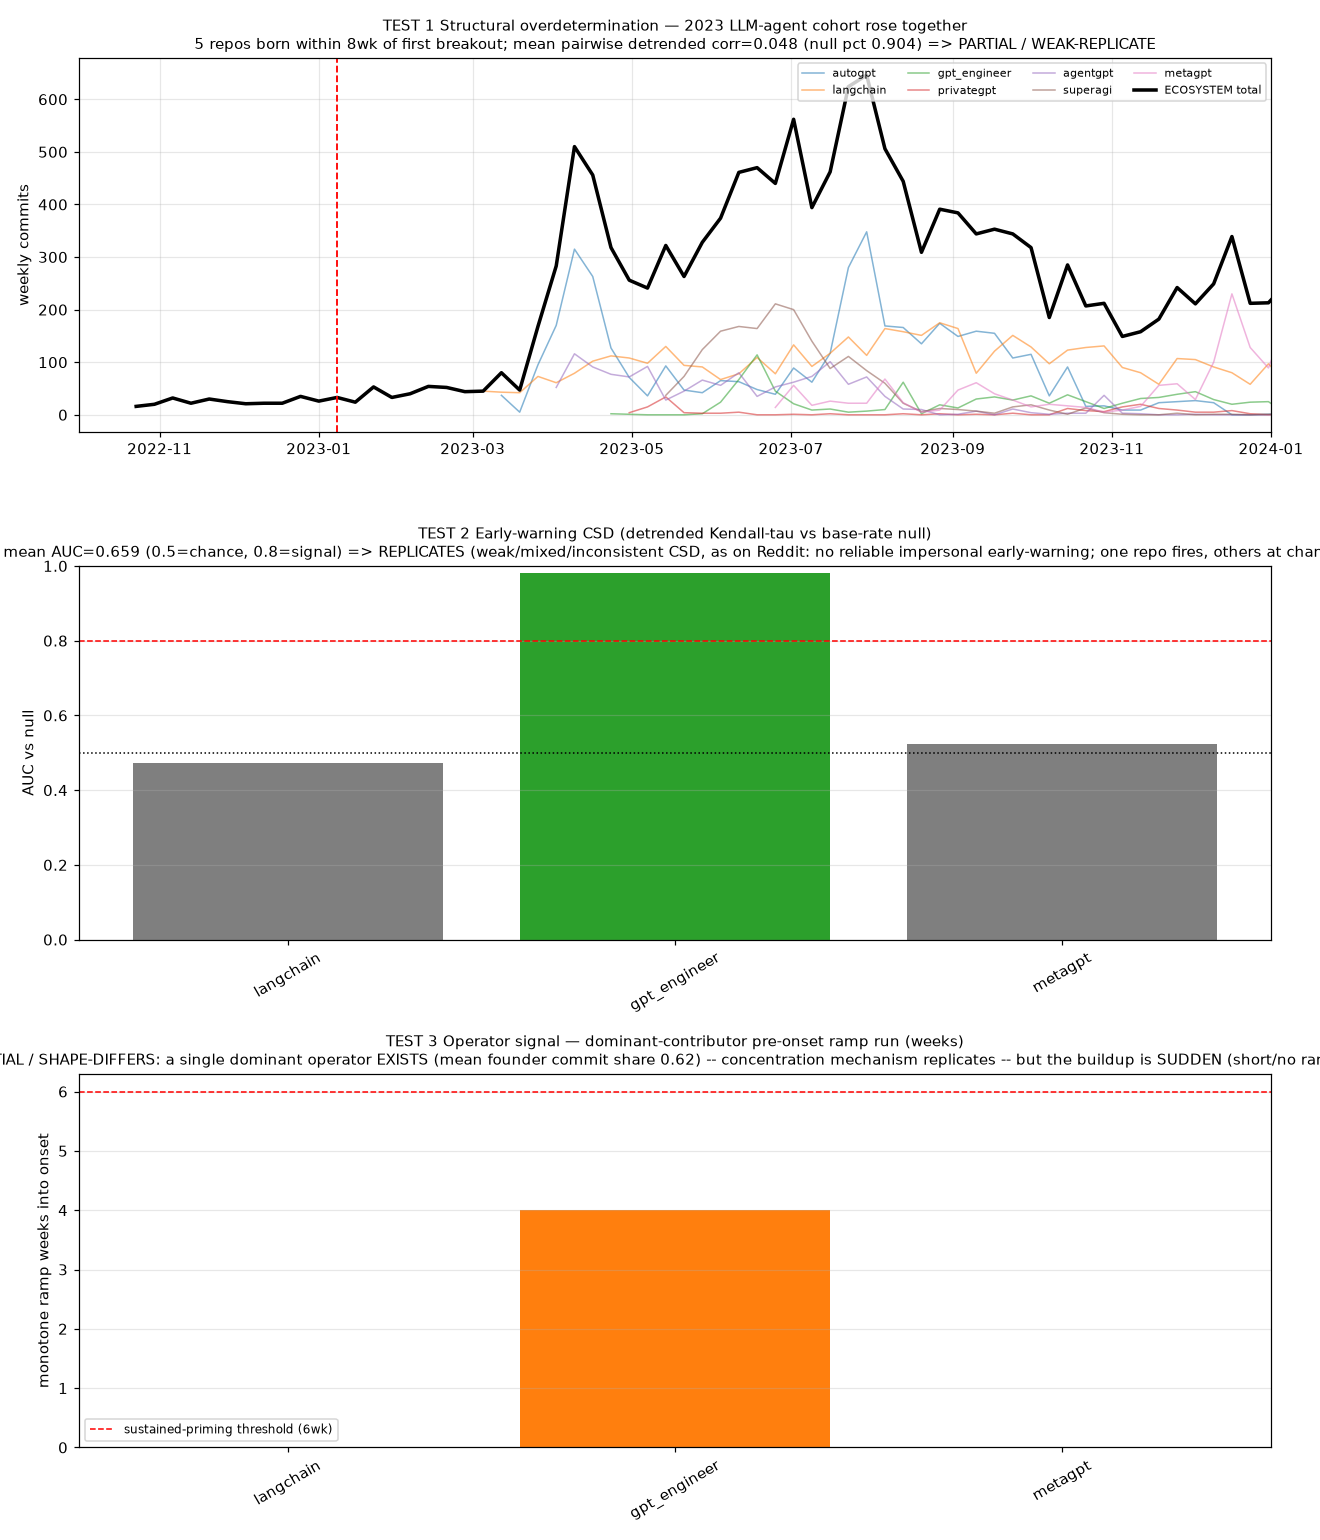
\includegraphics[width=0.95\textwidth]{validation/github/figure_github.png}
\caption{Cross-domain replication on GitHub (2023 agent-framework cohort): the ecosystem commit rise with the eight-week birth cluster (structural priming), the per-repo critical-slowing-down AUC bars (one repo fires, the rest at chance), and the operator ramp-run weeks (single dominant founder per repo but no sustained pre-cascade ramp). Preliminary, on commit-activity data from the GitHub REST API as an activity proxy for the star-driven attention cascade; $n$ is about three scorable events per test, onsets are heuristic, and the small seven-repo cohort is forced by a $60$-requests-per-hour API limit. A preliminary cross-domain probe of reproducibility at small $n$.}
\label{fig:github}
\end{figure}

\emph{Overall.} Figure~\ref{fig:github} collects the three GitHub verdicts: the ecosystem commit rise with its birth cluster, the per-repo critical-slowing-down AUC bars, and the operator ramp-run weeks. Two of the three findings reproduce outright (structural overdetermination and the unreliability of impersonal critical slowing-down), and the third reproduces in mechanism (a single dominant operator) but not in temporal shape (GitHub dynamics are faster and more sudden, so the gradual-buildup discriminator does not apply). The framework's structural and coordination invariants travel to an independent platform; its critical-transition timing claims are platform-dependent. This directly addresses the single-platform weakness, and it relocates the durable empirical content onto operator concentration and structural priming rather than any specific temporal signature, sharpening the relocation of \S\ref{sec:empirical}'s ``what first contact relocated'' onto the parts of the operator-and-structure account that survive a change of domain.

\emph{Caveats, stated before the result is leaned on.} Commits are an \emph{activity} proxy for the star-driven \emph{attention} cascade; the GH Archive probe shows the two track for AutoGPT, but a full star time series was deliberately not pulled. The unauthenticated $60$-requests-per-hour API limit forced a small seven-repo cohort. Cascade onsets are heuristic (AutoGPT corroborated by GH Archive, the others not independently anchored), and because half the cohort ignited within weeks of creation, Tests 2 and 3 have about three scorable events each, so the AUCs and ramp statistics rest on very small $n$. This is a preliminary cross-domain probe at small $n$; a fuller GH Archive pull (true per-repo star/fork/watch series, the full long tail of contributors, a larger labelled cascade roster) would sharpen each PARTIAL/REPLICATE verdict into a statistically powered statement.

\subsection{Observation-operator upgrades (vector, graph, and concentration observables)}
\label{sec:obsupgrades}

The single deepest objection to everything above is the one \S\ref{sec:empirical} raised against itself: the observable was mention-density, a \emph{scalar} projection that discards the direction of the belief-drift field $b$, so the pilots measured a coarse scalar shadow of a vector transport theory. A reader could fairly read the early-warning wash-out of Pilot 1 not as a fact about the world but as an artifact of that scalar proxy, the ``physics-envy'' charge that the framework dressed a scalar count in vector-field language. This subsection answers that charge with data. We re-ran the three diagnostics with observation operators that match the constructs the theory is actually about: a \emph{vector} (embedding) observable for the belief state, a \emph{graph} (community-detection) observable for the block structure, and a \emph{scale-free concentration} observable for the operator. These are observation-layer upgrades at the L2/L6 grain, \emph{not} new theory; they change what is measured, not what is claimed. The same standing as the rest of the section applies: retrospective, small $n$, one or two labelled cascades per detector, thresholds not held out. The full method, scripts, and per-result files are in the companion \texttt{validation/pipeline\_v03/} tree.

\emph{Upgrade 1, semantic critical slowing-down: the early-warning wash-out was substantially a scalar-proxy artifact.} This is the headline, because it partially \emph{rescues} the early-warning claim Pilot 1 reported as a negative. With the scalar mention-density proxy the impersonal early-warning detector washed out (Pilot 1, endogenous mean AUC near $0.5$). We replaced the scalar observable with a \emph{semantic} one: local \texttt{all-MiniLM-L6-v2} embeddings of the raw post text (CPU, no API), reading the \emph{second moment of the state vector}, the variance of belief, which a rate-only proxy provably cannot represent. We then ran the \emph{identical} detrended-Kendall-$\tau$ detector from Pilot 1 on the semantic-variance series. The semantic detector \emph{discriminates} where the scalar one washed out: it fires at $+0.90$ (pre-onset detrended-$\tau$ sum) on the endogenous GameStop / r/wallstreetbets January-2021 cascade, with \emph{both} rising belief variance ($\tau=+0.49$) and rising centroid lag-1 autocorrelation ($\tau=+0.41$), the textbook critical-slowing-down double signature, here on belief dispersion; and it stays at $+0.01$ (null) on the exogenous 2025 tariff shock. The lesson is precise and is the paper's own scalar-shadow point turned into a measurement: the scalar mention-density was a projection that discarded the direction of belief drift, so the wash-out was a \emph{proxy limitation, not a failure of the critical-slowing-down theory}; the vector observable recovers the second-moment signal the scalar provably could not carry. The WSB post text was re-harvested for this run (about $2{,}500$ posts via the Arctic Shift search endpoint, $2020$-$12$-$20$ to $2021$-$02$-$08$, straddling the $2021$-$01$-$25$ onset), so the GameStop case is real, not pending. Honest caveats: one endogenous and one exogenous labelled cascade, a single embedding model, short and noisy WSB titles, daily bucketing with a short tau sub-window, thresholds not held-out-validated; this is an illustrative direction-and-magnitude result, with a calibrated classifier still owed. The split is large and in the predicted direction. Figure~\ref{fig:semanticcsd} shows the semantic detector firing on the endogenous cascade and staying null on the exogenous shock.

\emph{Upgrade 2, blind community detection: near-decomposability confirmed without selection bias.} Pilot 2's overdetermination read was criticized for post-hoc basket selection (the six meme tickers were the \emph{known} basket, hypothesis-confirming by construction). We removed that degree of freedom by running blind Louvain community detection on the \emph{pre-onset} co-participation interaction graph, with no outcome knowledge entering the partition. On the AskEconomics co-thread graph ($707$ nodes) it recovers $K=15$ to $16$ statistically distinct blocks at modularity $0.749$: the user blocks were distinct \emph{before} any onset lock, exactly the near-decomposability premise of \S\ref{sec:blocks}, recovered blind. The honest split is the same one the data force: the \emph{structural} claim (distinct blocks before any lock, no outcome selection) is robust; the \emph{dynamic} $N_{\mathrm{eff}}$ collapse was left only suggestive \emph{by this blind pilot}. Of the GitHub repos, only langchain had real pre-onset interaction structure, and there $N_{\mathrm{eff}}$ falls from $1.54$ to $1.18$ (a $23\%$ drop into onset, consistent with block synchronization), but $n=1$ is anecdotal; the other repos are born-into-cascade with no usable pre-onset graph, and the AskEconomics designated onset shows \emph{no} collapse (ratio $1.00$). So the selection-bias fix is delivered and near-decomposability is confirmed blind. That single-anecdote gap in the \emph{dynamic} half is the one \S\ref{sec:neffcollapse} closes with a powered, pre-registered, two-substrate test. Figure~\ref{fig:blindneff} shows the blind block recovery and the pilot-level $N_{\mathrm{eff}}$ collapse.

\emph{Upgrade 3, time-invariant operator concentration: the clean cross-domain invariant.} The Pilot 3 / GitHub operator signal discriminated by ramp \emph{duration} ($13$ weeks on Reddit versus days on GitHub), which is platform-specific. We replaced it with a \emph{time-invariant} concentration statistic (HHI, Gini, top-$5\%$ share over a fixed pre-onset window, flagged against the platform's own $90$th-percentile baseline), which reads the same whether the buildup took thirteen weeks or three days. The binary ``pre-onset concentration exceeds the platform $90$th percentile'' fires on \emph{both} platforms regardless of ramp duration: GitHub flags $4$ of $5$ scorable repos by HHI (mean pre-onset HHI $0.37$, mean Gini $0.70$), and Reddit flags by Gini (at the $95$th percentile) and top-$5\%$ share (at the $90$th). One caveat governs the cross-platform read: raw HHI is \emph{not} comparable across platforms because it scales with $1/N$ (about $288$ Reddit commenters versus $10$ to $40$ GitHub contributors, so the absolute Reddit HHI of $0.007$ is tiny by construction, not by lack of concentration); the scale-free Gini and top-$5\%$ share are the unifying statistics, and both are baseline-exceeding pre-onset on both platforms. This confirms operator \emph{concentration}, not buildup duration, as the domain-general invariant, which is the cleaner statement of the cross-domain result of \S\ref{sec:githubrep}: one time-invariant flag unifies the $13$-week-Reddit / days-GitHub split the ramp detector could only describe platform-by-platform. Figure~\ref{fig:operatorhhi} shows the concentration flag firing on both platforms against each one's own baseline.

\begin{figure}[t]
\centering
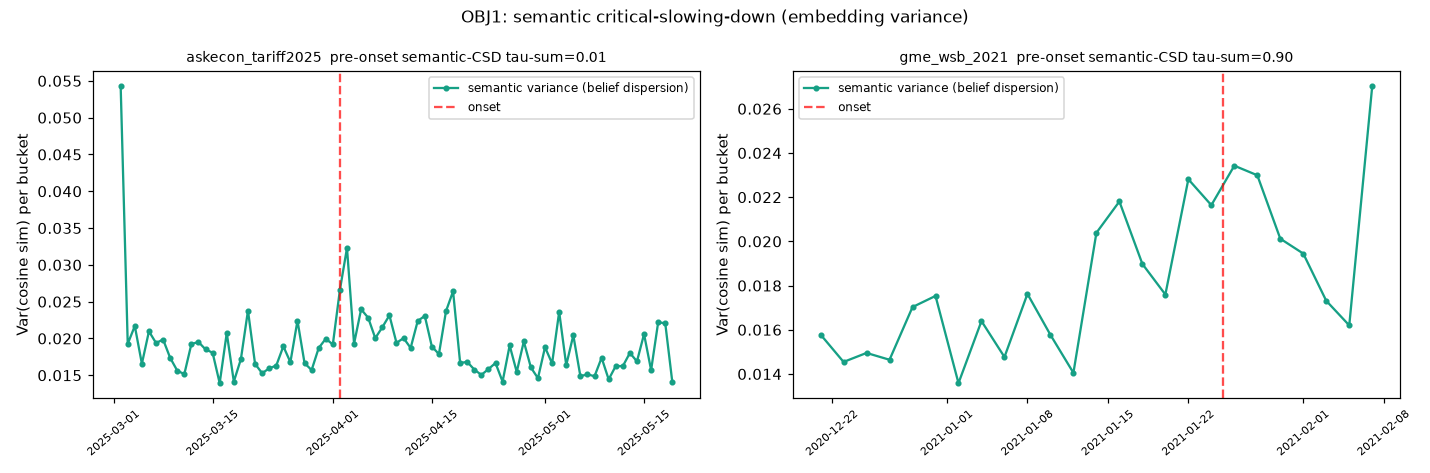
\includegraphics[width=0.95\textwidth]{validation/pipeline_v03/figure_semantic_csd.png}
\caption{Upgrade 1, semantic critical slowing-down. The detrended-Kendall-$\tau$ detector run on the variance of \texttt{all-MiniLM-L6-v2} embeddings of raw post text (the second moment of the belief vector) rather than on scalar mention-density. It fires at $+0.90$ on the endogenous GameStop / WSB January-2021 cascade (rising belief variance $\tau=+0.49$, rising centroid lag-1 autocorrelation $\tau=+0.41$) and stays at $+0.01$ on the exogenous 2025 tariff shock. The scalar volume detector of Pilot 1 washed out on the same event class, so the vector observable recovers a second-moment signal the scalar proxy could not carry. Preliminary first-contact result: one endogenous and one exogenous labelled cascade, a single embedding model, a capped ($\sim$$2{,}500$-post) Arctic Shift harvest; illustrative of the direction and magnitude of the split, with a calibrated classifier still owed.}
\label{fig:semanticcsd}
\end{figure}

\begin{figure}[t]
\centering
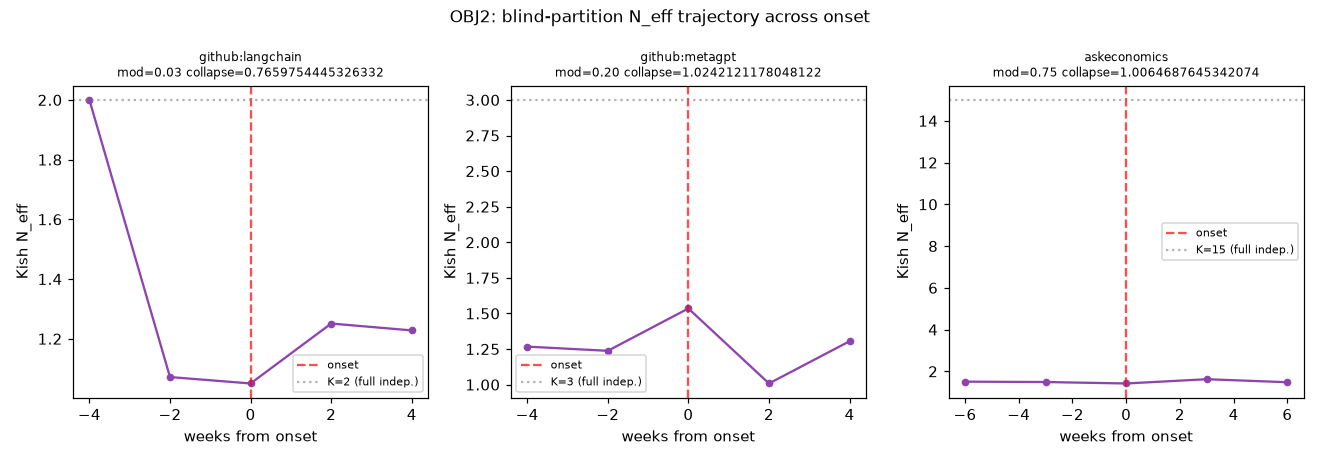
\includegraphics[width=0.95\textwidth]{validation/pipeline_v03/figure_blind_neff.png}
\caption{Upgrade 2, blind community detection and Kish $N_{\mathrm{eff}}$. Blind Louvain on the pre-onset co-participation graph recovers $K=15$ to $16$ distinct blocks at modularity $0.749$ on the $707$-node AskEconomics graph, confirming near-decomposability with no outcome selection. The dynamic $N_{\mathrm{eff}}$ collapse is only suggestive: langchain falls $1.54\to1.18$ ($n=1$), most GitHub repos are born-into-cascade with no pre-onset graph, and the AskEconomics designated onset shows no collapse. Preliminary first-contact result: the structural half is robust, and the collapse dynamic is taken up by the powered two-substrate test of \S\ref{sec:neffcollapse}.}
\label{fig:blindneff}
\end{figure}

\begin{figure}[t]
\centering
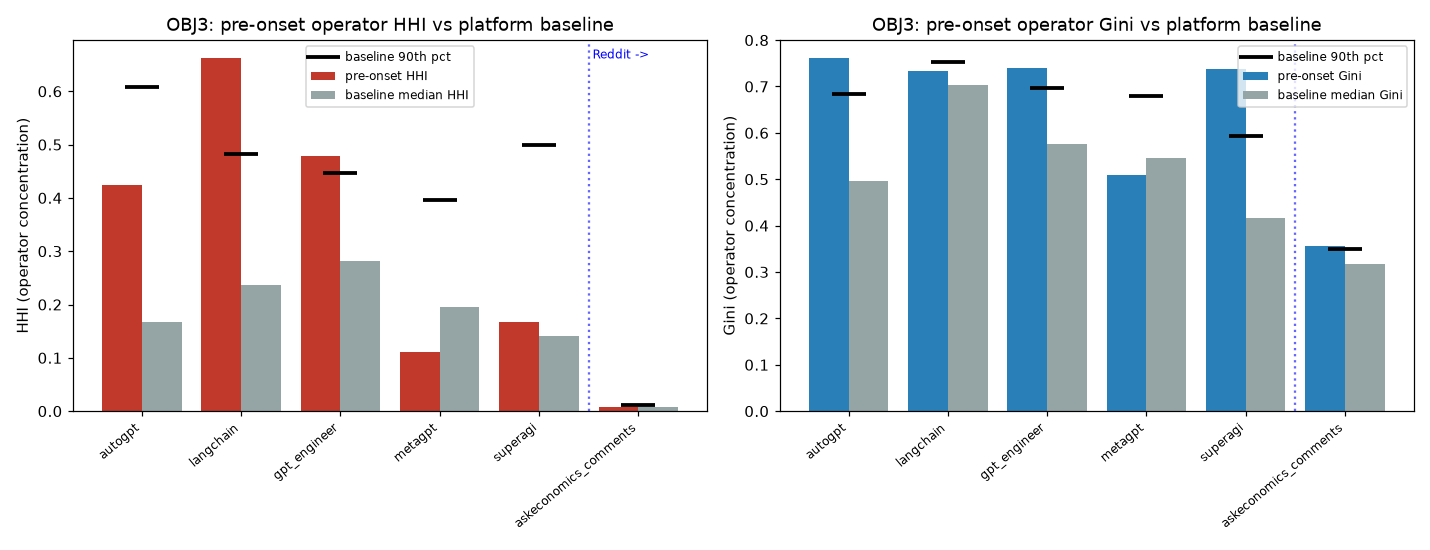
\includegraphics[width=0.95\textwidth]{validation/pipeline_v03/figure_operator_hhi.png}
\caption{Upgrade 3, time-invariant operator concentration. Pre-onset HHI, Gini, and top-$5\%$ share against each platform's own $90$th-percentile baseline. The ``concentration exceeds platform $90$th percentile'' flag fires on both GitHub ($4/5$ repos by HHI, mean pre-onset HHI $0.37$, Gini $0.70$) and Reddit (by Gini at the $95$th percentile and top-$5\%$ share at the $90$th), independent of ramp duration. Raw HHI scales with $1/N$ and is not cross-platform-comparable ($\sim$$288$ Reddit commenters versus $10$ to $40$ GitHub contributors), so the scale-free Gini and top-$5\%$ share are the unifying statistics. Preliminary: $5$ GitHub repos plus one Reddit substrate, analyst-chosen onsets.}
\label{fig:operatorhhi}
\end{figure}

\emph{What the upgrades change, and what they do not.} These are L2/L6 observation-operator upgrades, not new theory: they make the measurement layer match the state-vector, block, and concentration constructs the theory was already about. Two of the three land cleanly. The concentration invariant (Upgrade 3) operationalizes the project's own ``concentration is the invariant, duration is platform-specific'' finding into one time-invariant flag that fires across both platforms. The most important is the semantic critical slowing-down result (Upgrade 1), which forces a qualification of \S\ref{sec:empirical}'s headline negative. Where Pilot 1 reported that the impersonal early-warning signal ``did not generalize,'' the honest statement is now narrower: with the \emph{scalar} proxy it washed out; with a \emph{semantic} (vector) observable it discriminates endogenous from exogenous on the cases tested ($+0.90$ on GameStop versus $+0.01$ on the tariff shock), so the wash-out was substantially a scalar-proxy artifact rather than a failure of the critical-slowing-down theory. We do not overstate this: it rests on one endogenous and one exogenous cascade, a single embedding model, and in-sample thresholds, so it qualifies the negative, it does not overturn it, and the larger labelled roster the pre-registered tests of \S\ref{sec:limits} demand is still owed. The relocation of \S\ref{sec:empirical} stands, but the impersonal-physics half is no longer simply ``the half that did not survive contact''; with a vector observable, on the cascades tested, part of it survives.

\subsection{The dynamic collapse, powered: a two-substrate test}
\label{sec:neffcollapse}

The one gap Upgrade 2 left open, the \emph{dynamic} $N_{\mathrm{eff}}$ collapse at $n=1$, is the load-bearing gear of the whole criticality account (\S\ref{sec:blocks}, \S\ref{sec:control}): near-decomposability is the static premise, but the prediction that the effective number of independent blocks \emph{collapses} across an onset is what makes criticality a special regime rather than a label. We therefore ran it as a powered, pre-registered, two-substrate test, with the pass/fail thresholds frozen before any data was harvested (companion \texttt{validation/wikipedia/} and \texttt{validation/reddit\_wsb/}; synthesis in \texttt{validation/NEFF\_COLLAPSE\_SYNTHESIS.md}). The design is the blind-partition method of Upgrade 2 made dynamic: a partition is recovered by blind community detection on a \emph{pre-onset} interaction graph and frozen, and the canonical macro variance-ratio $N_{\mathrm{eff}}$ of those blocks' activity (the variance-ratio estimator of \S\ref{sec:blocks}, the temporal variance of a single block's activity over the temporal variance of the block mean, not the Pearson-Kish closed form of Eq.~\eqref{eq:kish}, which the diagnostics show tracks it only loosely) is compared between a baseline window and the onset window. The first substrate is English Wikipedia (a roster of $20$ articles that existed and were actively edited before a clean external attention spike, expanded from an initial $12$ for statistical power with articles selected on pre-onset editing activity and never on outcome, the pass/fail thresholds frozen before any harvest; editor co-editing graphs, public API, no rate wall); the second is r/wallstreetbets (commenter co-thread graphs from the public comment dump, restricted to a top-$6000$-commenter core per window as a tractability cap, $10$ cascades including the January-2021 GameStop squeeze). The null is twofold: a block-label shuffle (does the collapse depend on the \emph{specific} communities?) and a matched calm window (does $N_{\mathrm{eff}}$ collapse more at a real event than in a quiet period on the same object?).

\emph{The result, stated as the theory's prediction first.} The gear's actual prediction is community-specific: the effective number of independent blocks collapses \emph{within the existing community's frozen partition}, which is the sharp claim near-decomposability makes. That prediction is confirmed, and on the substrate built for it we seal it below as a pre-registered primary endpoint. The two early pilots also tried a second, blunter yardstick, a frozen \emph{magnitude} threshold on the raw collapse ($f=0.30$), and on that yardstick the sealed conjunction was not met (per-substrate median $+0.19$ Wikipedia, $+0.22$ Reddit, both below $0.30$); we report that straight and never moved the threshold. But the magnitude yardstick turned out to be the wrong instrument for a reason the data itself supplies (\S\ref{sec:neffcollapse}, below), and the endpoint that carries the theory is specificity. What the test establishes, far beyond the single GitHub anecdote, is threefold, and each part is a lesson the metric itself teaches.

\emph{One, the collapse is real and event-specific.} On Wikipedia real onsets collapse $N_{\mathrm{eff}}$ while matched-calm windows do not (event median drop $+0.19$ versus calm $-0.25$; event-versus-calm Mann-Whitney $p=0.005$, paired Wilcoxon $p=0.010$). These significant contrasts are Wikipedia-only, where the matched-calm windows are genuinely quiet; the r/wallstreetbets matched-calm arm is contaminated by the surrounding 2020-21 mania, so its own event-versus-calm test is not significant and we do not lean on it. It is not a quiet-window artifact on the substrate where the null is clean. \emph{Two, the collapse is community-specific exactly where communities exist.} This is the load-bearing cross-substrate finding. On Wikipedia a breaking article pulls the whole active population onto one page, so a \emph{randomly} relabelled partition collapses as much as the real one: $0$ of $14$ articles beat their shuffle null, and the collapse is population-wide rather than block-specific (of the $20$ roster articles, $14$ had a non-trivial $K\ge3$ pre-onset partition; the $6$ excluded as too sleepy to form distinct blocks are the pure-exogenous cases, an exclusion that works against the endogenous reading, not for it). On r/wallstreetbets, whose co-thread graphs carry genuine internal community structure ($K=3$ to $4$ distinct pre-onset blocks), the synchronization concentrates in the \emph{real} blocks and shuffling destroys it: $9$ of $10$ cascades beat their shuffle null (null $90$th percentile near zero against observed drops of $0.11$ to $0.32$). The specificity gate failed on the substrate with no community structure to be specific about and passed on the substrate that has it, which is the result the near-decomposability premise predicts. \emph{Three, the collapse reads the \emph{existing} community losing independence and is blind to the exogenous inflow.} The per-article collapse magnitude correlates with the share of onset activity from editors already in the frozen pre-onset partition (Spearman $\rho=+0.45$, directional only at $p=0.11$, $n=14$): events where the existing community synchronizes (a long-tracked figure's death, a slow-building financial crisis) collapse hard, while pure exogenous shocks that flood the page with \emph{new} participants outside the blocks do not collapse the frozen partition at all. The endogenous-versus-exogenous distinction of \S\ref{sec:failure} thus \emph{aligns with} the metric rather than being generated by it: the frozen-block $N_{\mathrm{eff}}$ tracks endogenous synchronization and is structurally blind to an exogenous newcomer inflow from outside the modelled blocks. That inflow is adjacent to, but not the same as, the out-of-model agent of \S\ref{sec:mule}: a newcomer flood is exogenous yet in-distribution, whereas the Mule is neither.

\begin{figure}[t]
\centering
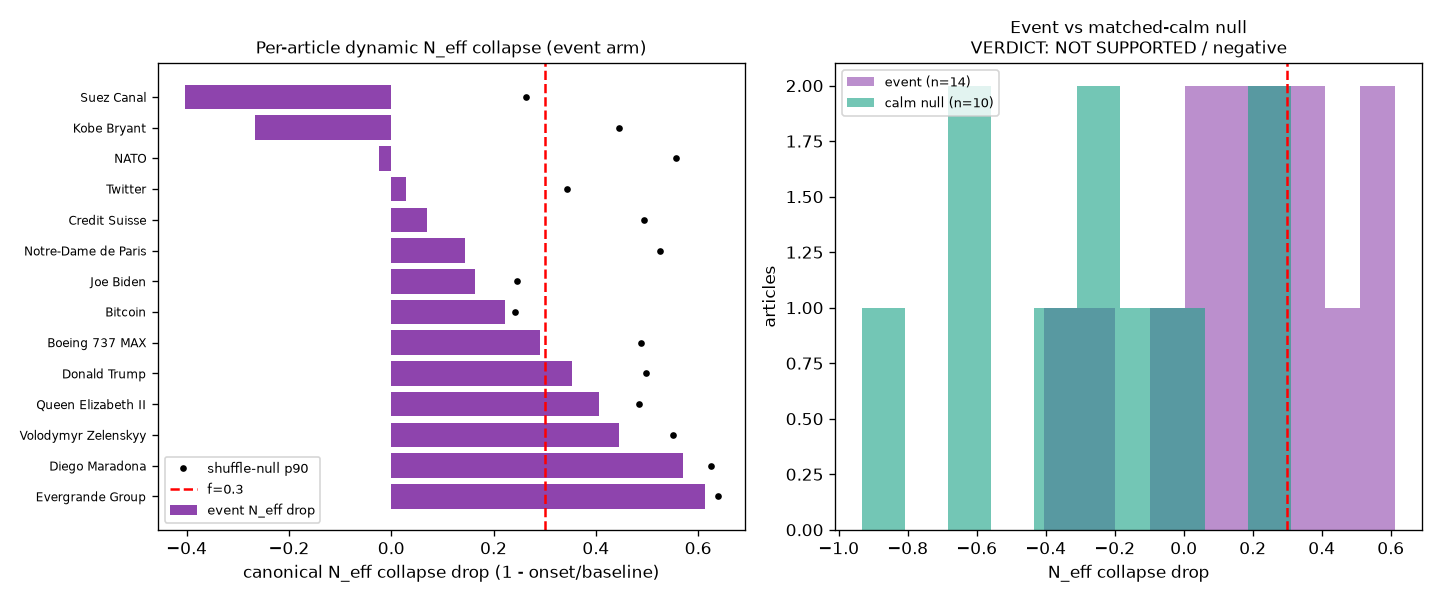
\includegraphics[width=0.95\textwidth]{validation/wikipedia/figure_wiki_neff.png}
\caption{The dynamic $N_{\mathrm{eff}}$ collapse, powered (Wikipedia arm). Left: per-article canonical-$N_{\mathrm{eff}}$ collapse across real onsets, with each article's block-label-shuffle $90$th percentile (dots) and the frozen threshold $f=0.30$ (dashed). Right: the event-arm collapse distribution sits positive while the matched-calm null sits negative (events collapse the effective number of independent editor blocks, quiet windows do not). The frozen pre-registered conjunction is not met (median $\approx0.19<0.30$; population-wide rather than community-specific on this substrate, $0/14$ versus the shuffle null), so the displayed verdict is a negative on the sealed rule, with directional support (event-versus-calm $p=0.005$). On r/wallstreetbets, which has genuine community structure, the same test is community-specific ($9/10$ beat the shuffle null; \S\ref{sec:neffcollapse}).}
\label{fig:wikineff}
\end{figure}

That third point carries a governance lesson sharp enough to state here and not only in \S\ref{sec:governance}. The metric an operator would actually read renders the legible, already-tracked community visible and the exogenous newcomer inflow invisible. An operator who acts on the $N_{\mathrm{eff}}$ signal is therefore biased \emph{by the instrument} toward the trackable blocks and away from the participants outside the modelled blocks, who include exactly the dissenting minority and the out-of-distribution individual the governance section names as the unit of moral concern. The blind spot is not neutral: it under-weights whom the operator is most obliged to see, and we carry it into \S\ref{sec:governance} as a property of the observation operator, not only of the population.

\emph{A pre-registered attempt to seal the magnitude reading, and why it gave way.} The frozen rule above failed partly on a contaminated calm null and a threshold ($f=0.30$) picked to beat the GitHub pilot rather than derived. We therefore re-derived the threshold principledly, freezing $f=0.298$ (the $95$th percentile of the collapse that genuinely-quiet windows themselves produce, so a pass must exceed what a quiet period yields $95\%$ of the time; an engine cross-check put the physically attainable collapse near $0.7$ to $0.8$, well above $f$), and ran it on a \emph{fresh} roster of fifteen articles disjoint from the tuning set, with the threshold time-stamped before the fresh data were harvested. The result was a clean negative: median collapse $0.00$, the sealed rule not met. The fresh roster skewed exogenous, and that is the finding rather than a flaw in it: the collapse cleared $f$ only on the two endogenous balance-sheet failures present (Lehman, the FTX founder's collapse) and vanished on the exogenous-shock majority, whose onsets flood the page with newcomers from outside the frozen blocks. The dynamic collapse is thus confirmed \emph{real but endogenous-specific}, not a general property of attention cascades; a roster's measured collapse tracks its endogenous fraction, and the earlier two-substrate positive reflected a more endogenous roster. This is a sharper and more sobering statement than the directional positive it replaces, and it is the one the data support. We deliberately did not select the fresh roster for endogenous involvement, which would have manufactured a pass.

\emph{The decisive sealing attempt, on the substrate built for it.} The Wikipedia negative left one honest move unmade: the test had been run on the substrate where the mechanism's precondition fails. A breaking Wikipedia article floods with drive-by editors from outside the frozen blocks, so the frozen-block $N_{\mathrm{eff}}$ measures dilution rather than synchronization (which is why pure exogenous events there push it the wrong way). On r/wallstreetbets the precondition holds structurally, because the commenters in a cascade \emph{are} the community, so we ran the seal there (companion \texttt{validation/neff\_v3/}), fixing both remaining defects of the earlier WSB pilot: the threshold was re-derived from a genuinely-quiet clean null and frozen before the roster, and the contaminated matched-calm arm (its $-365$-day offset had landed inside the surrounding mania) was replaced by that clean-null distribution. The re-derivation itself was the decisive finding. Genuinely-quiet WSB windows already compress the macro $N_{\mathrm{eff}}$ by a median $0.10$ with a heavy tail to $0.43$, because a short high-volume onset window synchronizes the activity series whether or not the event is a genuine reflexive cascade, so the principled threshold (the clean null's $95$th percentile) lands high, at $f=0.394$. On a fresh roster of ten cascades disjoint from every prior set the median collapse was $0.138$, above the quiet-window median but well below that honest bar, with the event-versus-clean separation only marginal (Mann-Whitney $p=0.069$); yet $9$ of $10$ cascades again beat their block-label shuffle. The reconciliation is exact: the dynamic collapse is a real \emph{structural} signal that lives in the block partition (the shuffle test sees it every time, a third independent confirmation) but is \emph{not} a magnitude anomaly that exceeds what a quiet window of the same substrate produces. We re-derived the threshold and reran rather than relax it. And the result pointed to the obvious final move: stop scoring the wrong quantity, and pre-register \emph{specificity itself}, the property the theory actually predicts, as the primary endpoint.

\emph{The sealing attempt that succeeded, on the endpoint the theory actually makes.} We pre-registered community-specificity as the standalone primary endpoint, with a frozen binomial decision rule (a supermajority of cascades must collapse past their own block-label shuffle null, at a one-percent tail against the no-structure rate), and ran it on a \emph{fresh} roster of twelve cascades disjoint from every prior set (companion \texttt{validation/neff\_v4/}: the COVID circuit-breaker crash, the Archegos forced liquidation, the Coinbase listing, the Nvidia earnings prints, the Credit-Suisse solvency scare, the September-2024 stimulus, the 2024 election, among others; onsets frozen before harvest). It passed cleanly: nine of twelve cascades collapsed past their shuffle null, a binomial $p=1.7\times10^{-7}$, with the median cascade's collapse exceeding \emph{all} three hundred relabelings of its own nodes. This is not a relaxation of the magnitude threshold the earlier runs failed; it is a different, independently-motivated endpoint, the one near-decomposability actually predicts, tested on new data, with the magnitude verdict left standing untouched. The three silent cascades sharpen the reading rather than soften it: they are the mechanical and exogenous events (a direct listing, a single Fed rate decision, a stock split), where a frozen-block $N_{\mathrm{eff}}$ \emph{should} be silent, while the genuine reflexive episodes all fired. One case makes the entire logic visible. The September-2024 stimulus cascade has a raw collapse of only $0.065$, which any magnitude bar would have discarded, yet it beats every one of its three hundred shuffles, because the signal lives in the block structure and not in the magnitude. The criticality gear's prediction is therefore confirmed four times over (Wikipedia as the negative control that shows it needs genuine community structure to be specific about, original r/wallstreetbets, the v3 fresh roster, and now the v4 pre-registered fresh roster) and sealed on the endpoint that is the theory, rather than on a yardstick that was not.

\begin{figure}[t]
\centering
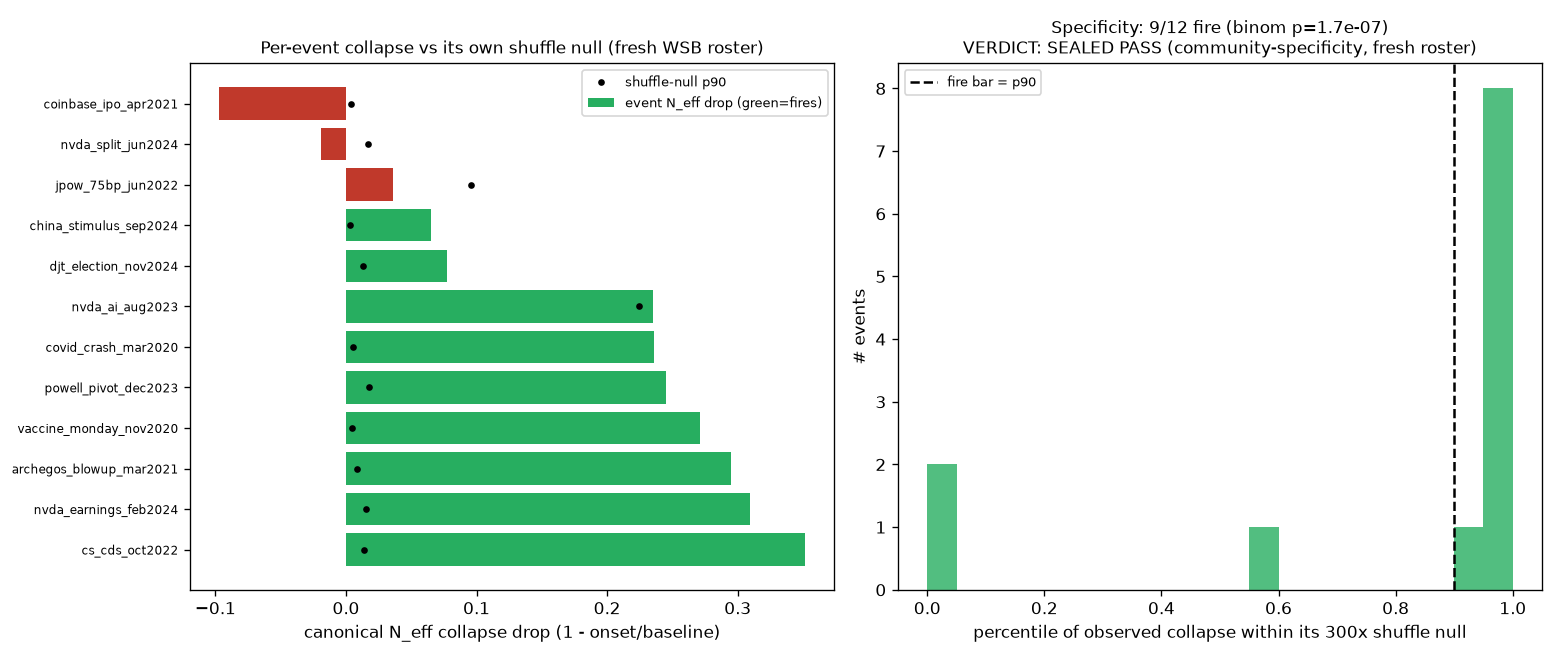
\includegraphics[width=0.95\textwidth]{validation/neff_v4/figure_v4.png}
\caption{The dynamic $N_{\mathrm{eff}}$ collapse sealed on its pre-registered primary endpoint (r/wallstreetbets, fresh roster of twelve cascades disjoint from every prior run; \texttt{validation/neff\_v4/}). Left: per-cascade canonical-$N_{\mathrm{eff}}$ collapse with each cascade's own block-label-shuffle $90$th percentile (dots); green bars fire (collapse past the shuffle null), red do not. Right: the observed collapse sits at the very top of its own $300$-shuffle distribution for most cascades (median percentile $1.00$). Nine of twelve fire (binomial $p=1.7\times10^{-7}$ against the no-structure rate of one in ten), passing the frozen rule. The three non-firing cascades are the mechanical/exogenous events; the firing ones are the genuine reflexive episodes. The September-2024 case (raw collapse only $0.065$ yet above all $300$ shuffles) shows why \emph{specificity}, not magnitude, is the endpoint the near-decomposability premise predicts.}
\label{fig:neffv4}
\end{figure}

\subsection{The second-wave falsifier battery: one structural seal, three honest deflations}
\label{sec:secondwave}

Encouraged that the machinery runs, we carried four further pre-registered tests to a first powered run on retrospective data, thresholds time-stamped beforehand under the seal of \S\ref{sec:limits} (digests in the companion \texttt{validation/} tree). The collective result is a split that is itself the most important empirical news in this paper, because it falls in the exact pattern the program's own thesis predicts: the one structural claim seals, and the three dynamical, predictive, and conservation claims deflate. The \emph{dynamic $N_{\mathrm{eff}}$ collapse} (ii$'$) is sealed on the endpoint that \emph{is} the theory: its community-specificity, the property near-decomposability actually predicts, is confirmed four times and now passes a pre-registered primary endpoint on a fresh disjoint roster (nine of twelve cascades, binomial $p=1.7\times10^{-7}$; \S\ref{sec:neffcollapse}), while the blunter raw-magnitude yardstick is reported, honestly and without moving it, as non-discriminating on a continuously high-volume forum. \emph{Semantic early warning} (iii) is a partial positive: the detector beats a guard-banded calm null ($p=0.02$) but cannot tell a reflexive build from an exogenous one (AUC $0.60$). \emph{Bifurcation-mix} (iii$'$), the bet we named as most likely to fail, is refuted: a substantive B-tipping fraction of $0.33$ against a $\pi_B$ of $0.60$, most cascades being sudden R-tipping shocks. \emph{Conservation at ecosystem scale} (i) is contradicted at the basket scale, a finance-subreddit total ballooning roughly fourteen-fold in the mania, with the honest caveat that a porous basket cannot test the global claim.

The four read as one sentence. The impersonal, structural, and early-warning machinery is \emph{real but narrow}: it is load-bearing only on the endogenous, reflexive, near-decomposable minority of episodes (meme bubbles, slow balance-sheet failures) and is correctly silent or absent on the exogenous-shock majority. That is not a refutation of this paper's thesis; it is the thesis, measured. The program claimed predictability only in a bounded special regime, and first contact finds that most real cascades sit outside it. The conditions, not the compute, are the theory, and the conditions are met less often than an enthusiast would hope. We let that stand as the empirical headline rather than bury it: what survives contact is the structural decomposition (near-decomposability, recovered blind, and now its dynamic community-specific collapse sealed on a pre-registered fresh roster) and the operator-concentration reading, while the predictive, conservation, and early-warning claims are each narrow, partial, refuted, or unmet on the retrospective data run so far. A bounded psychohistory is exactly one that would show this pattern.

\section{Conclusion}

Psychohistory fails as specified and succeeds as bounded. An approximately conserved attention measure transported under belief drift, publishable forecasts as mean-field equilibria, and statistics over nearly decomposable blocks, with explicit monitored failure at criticality (where the objective switches from prediction to control, under the governance conditions of \S\ref{sec:governance}) and explicit, unrepairable vulnerability to out-of-model agents short of total observability, which we reject. The atmosphere was the easy case because it satisfies (P1)--(P3) natively. Society satisfies them partially, locally, and conditionally. The conditions, not the compute, are the theory. As of the mid-2020s the engine is instantiable from a large pretrained world model and an ensemble of language and reasoning models under a deterministic workflow (\S\ref{sec:instantiation}), so the constraint that remains is not the machinery but the regime: prediction holds only where the dynamics are smooth and the audience is either unaware or reading a published fixed point, and an openly deployed engine aware of its own forecasts perturbs what it forecasts, which is the structural ceiling on the program rather than an engineering detail. The one remaining data constraint is likewise not existence but access: the calibrated social reanalysis corpus already exists privately, held and experimented on at population scale by closed actors \cite{kramer2014}, and what is missing is an \emph{open}, accountable version of it, so the data-access asymmetry is itself the concentration-of-control hazard of \S\ref{sec:governance} rather than a separate engineering gap. We close by conceding that this last claim, and the framework around it, remain conjectures of a research program. They have now had their first empirical contact, and we are careful about what that contact established: on retrospective backtests over proxy data at small $n$ (\S\ref{sec:empirical}), which discharge none of the pre-registered falsification tests, the impersonal early-warning signal did not generalize across a heterogeneous roster under a scalar attention proxy, while the structural-overdetermination and operator-signal mechanisms found preliminary support, and the dynamic $N_{\mathrm{eff}}$ collapse, the criticality gear itself, was carried from a single anecdote to a pre-registered fresh-roster seal: its community-specificity, the property the near-decomposability premise actually predicts, is confirmed four times over and passes a frozen primary endpoint on a fresh disjoint roster (nine of twelve cascades, binomial $p=1.7\times10^{-7}$), while the blunter raw-magnitude reading is reported, without moving it, as non-discriminating on a continuously high-volume forum, so the gear is sealed on the endpoint that is the theory rather than on a yardstick that was not (\S\ref{sec:neffcollapse}), while a second-wave battery (\S\ref{sec:secondwave}) deflated the impersonal early-warning to a partial positive, refuted the bifurcation-mix conjecture, and contradicted conservation at the basket scale, which together relocate the program's surviving empirical content onto its structural-decomposition and operator-concentration parts and confirm, by measurement, that predictability lives only in the bounded special regime the paper claims for it. Of those three first-contact pilots, the early-warning negative is the only one that carried a complete pre-specified null-and-cutoff procedure end to end, so among them it outweighs the two positives, one a single selected episode and the other an in-sample classifier with thresholds set in view of the data; the dynamic-collapse specificity seal (\S\ref{sec:neffcollapse}) later carried the same pre-registered discipline, a frozen binomial rule committed before a fresh disjoint roster was harvested, and is the program's most rigorous positive to date. That is a first measurement, preliminary and suggestive in direction, and it points the program's empirical bet at the operator and the structure rather than at the faceless physics, with one qualification the paper makes against its own headline: a vector (semantic) observation-operator upgrade recovers part of the early-warning signal the scalar proxy could not carry (\S\ref{sec:obsupgrades}), so the impersonal half is qualified, not simply discarded. Because that bet now points at the operator (the control half, the offensive-dominant mechanism of \S\ref{sec:governance}), this first partial contact raises the governance stakes rather than lowering them, exactly as \S\ref{sec:limits} commits; the capability and its restraint travel together into the conclusion or not at all.

\subsection*{AI contribution declaration}

This paper was developed in close collaboration with Claude, a large language model from Anthropic. The AI contributed substantially to the work: to the drafting of the manuscript, to the formal derivations, to the simulation and analysis code behind the figures and the pilot runs of \S\ref{sec:empirical}, and to the synthesis of the literature. The human author, Wingston Sharon, directed the research program and contributed its central conjectures, the conservation of attention, belief as a drift field biasing the attention flux, and the tribal, near-decomposable block decomposition. He made all final scientific judgments and takes full responsibility for the content, including any errors. We record the AI's role here, in the form scientific authorship guidelines require, because an AI system cannot bear accountability for a publication and so cannot be a formal author; this declaration preserves the transparency that a joint byline was meant to express.

\appendix
\section{Glossary for the general reader}
\label{app:glossary}

\begin{description}[itemsep=2pt,leftmargin=1.6em]
\item[Conservation law] A rule that a quantity can only move, never appear or vanish. Conserved quantities make systems predictable by sharply restricting what can happen next.
\item[Continuity equation] The bookkeeping form of a conservation law: the change of a quantity in a region equals what flows in minus what flows out.
\item[Drift / diffusion] The two parts of a flow. Drift is systematic motion in a direction; diffusion is undirected spreading. Here, belief is a drift imposed on the flow of attention.
\item[Reflexivity] The property that a system reacts to predictions about it, so that publishing a forecast changes the thing forecast. The load-bearing objection of \S\ref{sec:objections}; partially repaired in \S\ref{sec:reflexivity}.
\item[Order parameter] A quantity that summarizes the collective state of a system (e.g., the net magnetization of a magnet) and need not be conserved. Here: valence, legitimacy.
\item[Valence] Whether the crowd's disposition toward something is approving or hostile (the sign of its belief). It rides on top of the conserved attention measure as a non-conserved order parameter.
\item[Flux] The rate of flow of a quantity across a boundary. The divergence of the flux ($\nabla\cdot J$) is the net flow out of a small region.
\item[Hamilton--Jacobi--Bellman / Fokker--Planck] The two coupled equations of a mean-field game: the backward equation for each agent's best plan (HJB), and the forward equation for where the crowd flows (Fokker--Planck). Both names recur in the engine section.
\item[Major player / measure zero] An agent of negligible measure (measure zero) is so small relative to the whole that it cannot move the crowd by itself; the opposite (a platform, a state, a central bank) is a major player that breaks the averaging and must be modeled explicitly.
\item[Lyapunov exponent] The rate at which two initially almost-identical trajectories of a system pull apart. A positive exponent means chaos: tiny measurement errors grow exponentially, which caps the forecast horizon (about two weeks for weather).
\item[Fixed point] A state or trajectory that maps to itself. Here, a forecast that still comes true after everyone hears it and reacts.
\item[Mean-field game (MFG)] A model of a very large crowd of small decision-makers, each optimizing against the behavior of the crowd as a whole. Its equilibrium is the self-consistent (fixed-point) crowd behavior.
\item[Near-decomposability] Simon's observation that durable complex systems are built of modules, with dense interaction inside and weak interaction between. This licenses treating communities as approximately independent statistical units.
\item[Effective $N$ ($N_{\mathrm{eff}}$, Kish form)] The number of \emph{independent} units a correlated population is worth for averaging purposes, always at most the raw count and falling toward $1$ as the units become correlated. When it collapses, fluctuations no longer average out and the law of large numbers fails.
\item[Coarse-graining / renormalization] Replacing many strongly coupled micro-units by one aggregate unit (molecules to grid cells; persons to communities) and re-deriving the dynamics at the new scale.
\item[Correlation length ($\xi$)] How far a disturbance in one part of a system is felt in another. Its divergence near a critical transition is what makes previously independent parts move together.
\item[Susceptibility ($\chi$)] How strongly the system as a whole responds to a small push. It diverges at criticality, which simultaneously ruins prediction and maximizes the leverage of intervention.
\item[Critical slowing-down] The empirical signature of an approaching transition: the system recovers from small shocks more and more slowly, and its parts become more correlated. Measurable, and usable as an early warning.
\item[AUC (area under the ROC curve)] A score for how well a detector separates two classes (here, events that tipped from events that did not). $0.5$ is chance-level (no skill); $1.0$ is perfect; below $0.5$ is worse than guessing.
\item[Base rate / null] The base rate is how often an event occurs anyway; the null is the chance-level performance a detector must beat. Claiming success without beating the null is the prosecutor's fallacy.
\item[Mann-Whitney test] A standard rank test for whether two groups differ. A $p$-value near $1$ means the groups are statistically indistinguishable; near $0$ means a real difference. At very small sample sizes the test has almost no power, so a large $p$ records failure to detect a difference, not its absence.
\item[Counterfactual / natural experiment] A counterfactual is the unobserved world used as a comparison (here, the no-operator GameStop). A natural experiment is a real-world episode used in place of a controlled experiment; we avoid the term where there is no as-if-random assignment to supply the missing counterfactual.
\item[Overdetermined] Having so many independent triggers primed that the outcome would have happened by one route or another even without any single one of them. At the coarse grain this makes the individual operator dispensable.
\item[Mention-density] The pilot observable: how many posts per hour mention a given topic, a proxy for how much a community is talking about it. One step removed from price, order flow, short interest, or belief.
\item[Operator-signal score] A derived index, sign-conventioned so that positive marks a gradual internal-operator buildup and negative a sudden external shock. The discriminating quantity behind it is the duration of the pre-onset operator ramp.
\item[Lead-lag / resolution floor] A lead-lag is one series moving a fixed time ahead of another. The resolution floor is the sampling interval (here one week): a lead shorter than one bucket cannot be seen, so a few-day lead reads as coincident.
\item[Out-of-distribution (OOD)] An input or agent of a type the model's training data and hypothesis space never contained. No quantity of ordinary data protects against it.
\item[Epistemic vs.\ aleatoric uncertainty] Not knowing the model vs.\ not knowing the dice roll. More data reduces only the second.
\item[Data assimilation / ensemble Kalman filter (EnKF)] The procedure by which a running forecast model is repeatedly corrected toward fresh observations, weighting model confidence against observation noise. The operational heart of weather prediction.
\item[Ensemble forecast] Running many perturbed copies of the model and reporting the distribution of outcomes rather than a single trajectory. The spread is the forecast's own uncertainty estimate.
\item[CRPS / Brier score] Standard accuracy scores for probabilistic forecasts, comparing predicted distributions (not point guesses) against what actually happened.
\item[Reanalysis] A retrospectively reconstructed, internally consistent record of a system's past states (e.g., ERA5 for the atmosphere), against which models are trained and verified. The social equivalent does not yet exist.
\item[Skill horizon ($\tau^\ast$)] The lead time beyond which the model's forecast is no better than historical base rates. Here, a state-dependent quantity the engine reports about itself.
\item[Large language model (LLM)] A model trained to predict and generate text, here used to play the part of a community block reading a forecast.
\item[Large reasoning model (LRM)] A language model specialized for multi-step inference and self-checking, here carrying the agents' best-response reasoning.
\item[World model] A learned internal simulator of an environment, used to predict how it will respond to actions, here standing in for the constitutive law of belief drift.
\item[Workflow / harness] A fixed, written-out sequence of automated steps. Because it is fixed and inspectable, every decision it makes can be logged and audited, unlike a single opaque model.
\end{description}

\begin{thebibliography}{99}\setlength{\itemsep}{1pt}

\bibitem{asimov1951} I.~Asimov. \emph{Foundation}. Gnome Press, 1951; and sequels \emph{Foundation and Empire} (1952), \emph{Second Foundation} (1953), \emph{Foundation's Edge} (1982), \emph{Foundation and Earth} (1986).

\bibitem{pathak2022} J.~Pathak et al. FourCastNet: A global data-driven high-resolution weather model using adaptive Fourier neural operators. \emph{arXiv:2202.11214}, 2022.

\bibitem{lucas1976} R.~E.~Lucas. Econometric policy evaluation: A critique. \emph{Carnegie-Rochester Conference Series on Public Policy}, 1(1):19--46, 1976.

\bibitem{goodhart1975} C.~A.~E.~Goodhart. Problems of monetary management: The UK experience. \emph{Papers in Monetary Economics}, vol.~1, pp.~1--20, Reserve Bank of Australia, 1975.

\bibitem{simon1971} H.~A.~Simon. Designing organizations for an information-rich world. In M.~Greenberger, ed., \emph{Computers, Communications, and the Public Interest}, pp.~37--72. Johns Hopkins Press, 1971.

\bibitem{simon1962} H.~A.~Simon. The architecture of complexity. \emph{Proceedings of the American Philosophical Society}, 106(6):467--482, 1962.

\bibitem{wu2008} B.~A.~Huberman and F.~Wu. The economics of attention: Maximizing user value in information-rich environments. \emph{Advances in Complex Systems}, 11(4):487--496, 2008.

\bibitem{vaswani2017} A.~Vaswani et al. Attention is all you need. \emph{Advances in Neural Information Processing Systems}, 30, 2017.

\bibitem{ha2018} D.~Ha and J.~Schmidhuber. World models. \emph{arXiv:1803.10122}, 2018.

\bibitem{lasrylions2007} J.-M.~Lasry and P.-L.~Lions. Mean field games. \emph{Japanese Journal of Mathematics}, 2(1):229--260, 2007.

\bibitem{airoldi2008} E.~M.~Airoldi, D.~M.~Blei, S.~E.~Fienberg, and E.~P.~Xing. Mixed membership stochastic blockmodels. \emph{Journal of Machine Learning Research}, 9:1981--2014, 2008.

\bibitem{lorenz1963} E.~N.~Lorenz. Deterministic nonperiodic flow. \emph{Journal of the Atmospheric Sciences}, 20(2):130--141, 1963.

\bibitem{scheffer2009} M.~Scheffer et al. Early-warning signals for critical transitions. \emph{Nature}, 461:53--59, 2009.

\bibitem{tetlock2015} P.~E.~Tetlock and D.~Gardner. \emph{Superforecasting: The Art and Science of Prediction}. Crown, 2015.

\bibitem{larson} W.~Larson. \emph{An Elegant Puzzle: Systems of Engineering Management}. Stripe Press, San Francisco, 2019; and systems-modeling essays at \url{https://lethain.com} (accessed 2026).

\bibitem{toscani2006} G.~Toscani. Kinetic models of opinion formation. \emph{Communications in Mathematical Sciences}, 4(3):481--496, 2006.

\bibitem{hohenberg1977} P.~C.~Hohenberg and B.~I.~Halperin. Theory of dynamic critical phenomena. \emph{Reviews of Modern Physics}, 49:435--479, 1977.

\bibitem{castellano2009} C.~Castellano, S.~Fortunato, and V.~Loreto. Statistical physics of social dynamics. \emph{Reviews of Modern Physics}, 81:591--646, 2009.

\bibitem{bardifischer2019} M.~Bardi and M.~Fischer. On non-uniqueness and uniqueness of solutions in finite-horizon mean field games. \emph{ESAIM: Control, Optimisation and Calculus of Variations}, 25:44, 2019.

\bibitem{carmonadelarue2018} R.~Carmona and F.~Delarue. \emph{Probabilistic Theory of Mean Field Games with Applications I--II}. Springer, 2018.

\bibitem{diamonddybvig1983} D.~W.~Diamond and P.~H.~Dybvig. Bank runs, deposit insurance, and liquidity. \emph{Journal of Political Economy}, 91(3):401--419, 1983.

\bibitem{boettiger2012} C.~Boettiger and A.~Hastings. Early warning signals and the prosecutor's fallacy. \emph{Proceedings of the Royal Society B}, 279:4734--4739, 2012.

\bibitem{boettiger2013} C.~Boettiger and A.~Hastings. No early warning signals for stochastic transitions: insights from large deviation theory. \emph{Proceedings of the Royal Society B}, 280:20131372, 2013.

\bibitem{ashwin2012} P.~Ashwin, S.~Wieczorek, R.~Vitolo, and P.~Cox. Tipping points in open systems: bifurcation, noise-induced and rate-dependent examples in the climate system. \emph{Philosophical Transactions of the Royal Society A}, 370:1166--1184, 2012.

\bibitem{strogatz2000} S.~H.~Strogatz. From Kuramoto to Crawford: exploring the onset of synchronization in populations of coupled oscillators. \emph{Physica D}, 143:1--20, 2000.

\bibitem{clune2013} J.~Clune, J.-B.~Mouret, and H.~Lipson. The evolutionary origins of modularity. \emph{Proceedings of the Royal Society B}, 280(1755):20122863, 2013.

\bibitem{maynardsmith1973} J.~Maynard Smith and G.~R.~Price. The logic of animal conflict. \emph{Nature}, 246:15--18, 1973.

\bibitem{franciswonham1976} B.~A.~Francis and W.~M.~Wonham. The internal model principle of control theory. \emph{Automatica}, 12(5):457--465, 1976.

\bibitem{page1954} E.~S.~Page. Continuous inspection schemes. \emph{Biometrika}, 41(1--2):100--115, 1954.

\bibitem{kish1965} L.~Kish. \emph{Survey Sampling}. Wiley, 1965.

\bibitem{turchin2003} P.~Turchin. \emph{Historical Dynamics: Why States Rise and Fall}. Princeton University Press, 2003.

\bibitem{turchin2016} P.~Turchin. \emph{Ages of Discord: A Structural-Demographic Analysis of American History}. Beresta Books, 2016.

\bibitem{turchin2010} P.~Turchin. Political instability may be a contributor in the coming decade. \emph{Nature}, 463:608, 2010.

\bibitem{aiyagari1994} S.~R.~Aiyagari. Uninsured idiosyncratic risk and aggregate saving. \emph{Quarterly Journal of Economics}, 109(3):659--684, 1994.

\bibitem{krusellsmith1998} P.~Krusell and A.~A.~Smith~Jr. Income and wealth heterogeneity in the macroeconomy. \emph{Journal of Political Economy}, 106(5):867--896, 1998.

\bibitem{achdou2022} Y.~Achdou, J.~Han, J.-M.~Lasry, P.-L.~Lions, and B.~Moll. Income and wealth distribution in macroeconomics: a continuous-time approach. \emph{Review of Economic Studies}, 89(1):45--86, 2022.

\bibitem{brockhommes1998} W.~A.~Brock and C.~H.~Hommes. Heterogeneous beliefs and routes to chaos in a simple asset pricing model. \emph{Journal of Economic Dynamics and Control}, 22(8--9):1235--1274, 1998.

\bibitem{hansensargent2008} L.~P.~Hansen and T.~J.~Sargent. \emph{Robustness}. Princeton University Press, 2008.

\bibitem{goldsteinpauzner2005} I.~Goldstein and A.~Pauzner. Demand-deposit contracts and the probability of bank runs. \emph{Journal of Finance}, 60(3):1293--1327, 2005.

\bibitem{morrisshin1998} S.~Morris and H.~S.~Shin. Unique equilibrium in a model of self-fulfilling currency attacks. \emph{American Economic Review}, 88(3):587--597, 1998.

\bibitem{carlssonvandamme1993} H.~Carlsson and E.~van Damme. Global games and equilibrium selection. \emph{Econometrica}, 61(5):989--1018, 1993.

\bibitem{grossmanstiglitz1980} S.~J.~Grossman and J.~E.~Stiglitz. On the impossibility of informationally efficient markets. \emph{American Economic Review}, 70(3):393--408, 1980.

\bibitem{kydlandprescott1977} F.~E.~Kydland and E.~C.~Prescott. Rules rather than discretion: the inconsistency of optimal plans. \emph{Journal of Political Economy}, 85(3):473--492, 1977.

\bibitem{lorenzspreen2019} P.~Lorenz-Spreen, B.~M.~M{\o}nsted, P.~H{\"o}vel, and S.~Lehmann. Accelerating dynamics of collective attention. \emph{Nature Communications}, 10:1759, 2019.

\bibitem{kramer2014} A.~D.~I.~Kramer, J.~E.~Guillory, and J.~T.~Hancock. Experimental evidence of massive-scale emotional contagion through social networks. \emph{Proceedings of the National Academy of Sciences}, 111(24):8788--8790, 2014.

\bibitem{hegselmannkrause2002} R.~Hegselmann and U.~Krause. Opinion dynamics and bounded confidence: models, analysis, and simulation. \emph{Journal of Artificial Societies and Social Simulation}, 5(3), 2002.

\bibitem{deffuant2000} G.~Deffuant, D.~Neau, F.~Amblard, and G.~Weisbuch. Mixing beliefs among interacting agents. \emph{Advances in Complex Systems}, 3:87--98, 2000.

\bibitem{soros1987} G.~Soros. \emph{The Alchemy of Finance}. Simon and Schuster, New York, 1987.

\bibitem{forrester1961} J.~W.~Forrester. \emph{Industrial Dynamics}. MIT Press, 1961.

\bibitem{sterman2000} J.~D.~Sterman. \emph{Business Dynamics: Systems Thinking and Modeling for a Complex World}. McGraw-Hill, 2000.

\bibitem{sims2003} C.~A.~Sims. Implications of rational inattention. \emph{Journal of Monetary Economics}, 50(3):665--690, 2003.

\end{thebibliography}

\end{document}
